% documentclass
% set font size=11 (11pt)
% set paper format=A4 (a4paper)
\documentclass[11pt,a4paper]{article}

%---------------
%   preamble   -
%---------------

% use the inputenc and fontenc packages to use French accents
\usepackage[utf8]{inputenc}
\usepackage[T1]{fontenc}

% use the babel package to handle the typographical rules and hyphenation patterns of the English language
\usepackage[english]{babel}

% allow for arbitrary font size
\usepackage{anyfontsize}

% set the font as Time New Roman (the Latex equivalent, at least)
\usepackage{mathptmx}

% set the size of the document margins using the geometry package
\usepackage[lmargin=0.95in,rmargin=0.95in,tmargin=1in,bmargin=1in]{geometry}

% turn the color of footnote markers to black
\renewcommand\thefootnote{\textcolor{black}{\arabic{footnote}}}
% suppress indents on footnotes
\usepackage[hang,flushmargin]{footmisc}

% automatically generates colored brackets around references
\usepackage{fncylab} \labelformat{equation}{(#1)}

% suppress indent on new paragraphs

\setlength{\parindent}{0pt}

% customize the bibliography by using the natbib package
\usepackage{natbib, url}
\bibliographystyle{plainnat} % was apa

% use the multirow package to be able to merge rows in tables
\usepackage{multirow}

% use the enumitem package to include enumeration options
\usepackage{enumitem}

% use the booktabs package to create nice-looking, customized tables
\usepackage{booktabs}

% use float package to force figure to be positioned where indicated
\usepackage{float}

% use makecell package to use forced line breaks within individual cells in tables
\usepackage{makecell}

% use the rotating package to be able to rotate a table
\usepackage{rotating}

% use the graphicx package to be able to resize tables
\usepackage{graphicx}
\graphicspath{ {./images/} }

% use the color package to be able to color text
\usepackage{color}

% Use the caption package to customize captions (titles) of tables and graphs
\usepackage[font=bf,labelfont=bf,justification=centering]{caption}

% Use the subcaption package to use captions for figures with multiple panels
\usepackage{subcaption}

% set options for subfigure captions
%\captionsetup[subfigure]{labelfont=normalfont,textfont=normalfont}

% allow for equation cross-referencing (hyperlinks)
\usepackage[colorlinks=true,allcolors=black]{hyperref}

% use the amsmath package to use all sorts of math symbols
\usepackage{amsmath}

% use the ammssymb package to use mathematical symbols
\usepackage{amssymb}
% create new commands for mathematical symbols
\DeclareMathOperator{\N}{\mathbb{N}}
\DeclareMathOperator{\Z}{\mathbb{Z}}
\DeclareMathOperator{\Q}{\mathbb{Q}}
\DeclareMathOperator{\R}{\mathbb{R}}
\DeclareMathOperator{\Pb}{\mathbb{P}}
\DeclareSymbolFont{epsilon}{OML}{ntxmi}{m}{it}
\DeclareMathSymbol{\epsilon}{\mathord}{epsilon}{"0F}
% declare the cmsy (computer modern symbol) math alphabet to define appropriate fonts for the U and N mathematical symbols
\DeclareMathAlphabet\mathbcal{OMS}{cmsy}{m}{n}
% create new commands for mathematical symbols
\DeclareMathOperator{\E}{\mathbcal{E}}
\DeclareMathOperator{\Ex}{\mathbb{E}}
\DeclareMathOperator{\F}{\mathbcal{F}}
\DeclareMathOperator{\G}{\mathbcal{G}}
\DeclareMathOperator{\M}{\mathbcal{M}}
\DeclareMathOperator{\HH}{\mathbcal{H}}
\DeclareMathOperator{\QQ}{\mathbcal{Q}}
\DeclareMathOperator{\PP}{\mathbcal{P}}
\DeclareMathOperator{\Noo}{\mathbcal{N}}
\DeclareMathOperator{\U}{\mathbcal{U}}
% use the bbm package to be able to use the double stroke 1 for the indicator function
\usepackage{bbm}
\DeclareMathOperator{\ind}{\mathbbmss{1}}

% use the bm package to use bold characters in math mode
\usepackage{bm}

% use the relsize package to be abe to change the size of mathematical symbols
\usepackage{relsize}

% define a new command for in-line small summation
\newcommand{\ssumm}[2]{\underset{\scriptscriptstyle #1}{\overset{\scriptscriptstyle #2}{\mathlarger{\mathlarger{\mathlarger{\Sigma}}}}} \hspace{0.5mm}}
% define a new command for in-line small products
\newcommand{\sprod}[2]{\underset{\scriptscriptstyle #1}{\overset{\scriptscriptstyle #2}{\mathlarger{\mathlarger{\mathlarger{\Pi}}}}} \hspace{0.5mm}}

% use the dcolumn package to align table entries on decimal separators
\usepackage{dcolumn}
\newcolumntype{d}[1]{D{.}{}{#1}}  % define "d" column type
\newcommand\mc[1]{\multicolumn{1}{c}{#1}} % handy shortcut macro

% create a new command for text superscript and subscripts (like 1st, 2nd, and so on)
\newcommand{\ts}{\textsuperscript}
\newcommand{\tb}{\textsubscript}

% use the mathtools package to use the matrix* environment, allowing to align matrix entries
\usepackage{mathtools}

% use tocloft package to set dotted lines in the table of contents
\usepackage{tocloft}
\renewcommand\cftsecfont{\normalfont}
\renewcommand\cftsecpagefont{\normalfont}
\renewcommand{\cftsecleader}{\cftdotfill{\cftsecdotsep}}
\renewcommand\cftsecdotsep{\cftdot}
\renewcommand\cftsubsecdotsep{\cftdot}

% manage paragraph line breaks
\usepackage{parskip}

% To get proper underline
\usepackage{soul}


%------------------------
%     main document     -
%------------------------


\begin{document}
	

%----------------------
%      title page     -
%----------------------


\begin{titlepage}
	
	\begin{textblock}{200}(1,1.2)
		{\transparent{0.7}
\includegraphics[width=1.2in, height=1.2in]{images/logotelecom.png}}
	\end{textblock}
		
	\begin{textblock}{200}(6.1,1.2)
		{\transparent{0.7}
\includegraphics[width=1.2in, height=1.2in]{images/logocfm.png}}
	\end{textblock}

	\vspace*{45mm}
	
	\begin{center}
		
		{\fontsize{18}{26}\selectfont Telecom Paris} \vspace{5mm}
		
		{\fontsize{18}{26}\selectfont Capital Fund Management} \vspace{10mm}

		\begin{titlepagebox}
			
			\setstretch{3}\begin{center}
				\textbf{{\fontsize{24}{26}\selectfont Professional thesis:}}
				
				\textbf{{\fontsize{24}{26}\selectfont Forecasting Economic Activity}}	
			\end{center}
				
		\end{titlepagebox} \vspace{10mm}
	
	
		{\fontsize{18}{26}\selectfont Romain Legrand} \vspace{2mm}
		
		{\fontsize{18}{26}\selectfont MS Big Data} \vspace{2mm}
		
		{\fontsize{18}{26}\selectfont 2019 - 2020} \vspace{15mm}
		
		\begin{titlepagephantombox}
	
			\setstretch{2}\begin{center}
				
				{\fontsize{16}{26}\selectfont Academic Supervisor:}
				{\fontsize{16}{26}\selectfont David Bounie}
				
			\end{center}
			
			
		\end{titlepagephantombox} \hspace{15mm}	
		\begin{titlepagephantombox}
	
			\setstretch{2}\begin{center}
				
				{\fontsize{16}{26}\selectfont Professional supervisor:}
				{\fontsize{16}{26}\selectfont Agustin Lifschitz}
					
			\end{center}
			
		\end{titlepagephantombox}
	
	\end{center}
	
\end{titlepage}

\cleardoublepage
	

%------------------------
%   table of contents   -
%------------------------
	
	
\tableofcontents
\pagebreak


%-------------------
%     sections     -
%-------------------


\section{Introduction}
\label{sec1}


Modern neural networks are the cornerstone of deep learning. The first representations of neural networks can be traced back to the early 1960's with the perceptron (\cite{Rosenblatt1958}) and Adaline/Madaline (\cite{Widrow1960}). These preliminary versions comprised only one layer and were limited to the solution of linear problems. However, many problems are non-linear by nature, so that the interest in perceptron models rapidly declined, leading to the beginning of the first AI winter.


The 1980's witnessed renewed interest in learning models. The seminal paper of \cite{Rumelhart1986} introduced multiple layers perceptron, eventually expanding neural networks to nonlinear domains. It also popularised the mechanism of training by backpropagation initially developed by \cite{Werbos1974}. At the same time, the neocognitron of \cite{Fukushima1980} constituted the first attempt at building a convolution neural network. The initial model was then extended to multi-layer settings and gradient methods by the contributions of \cite{LeCun1989} and \cite{LeCun1998}. In parallel, mathematicians started to build firm theoretical foundations for multi-layer perceptrons. \cite{Hornik1991} showed with appropriate weights, a single hidden layer neural network could approximate an arbitrary nonlinear function.


Despite those advance, interest in AI declined again at the end of the 1980's and machine learning entered its second winter. Neural networks in particular were deemed to be inefficient in practice, and support vector machines became the workhorse of machine learning. This long winter ended at the beginning of the 2010's through two major events. In 2011, Microsoft Research presented at the 12\ts{th} annual Conference of the International Speech Communication Association a neural network which dramatically improved speech recognition performance (\cite{Seide2011}). In 2012, the convolutional neural network AlexNet (\cite{Krizhevsky2012}) won the  ImageNet Large Scale Visual Recognition Challenge, outperforming by far its SVM challengers. These two events provided undeniable evidence that technological advance, in particular the improvement of GPUs, had rendered possible the training of sophisticated and highly efficient neural networks.


Since then, neural networks have proved immensely successful. They have been widely adopted and effectively used in fields as diverse as computer vision (\cite{Szegedy2015}), medical research (\cite{Levy2016}), astronomy (\cite{Dieleman2014}), image captioning (\cite{Karpathy2015}), and even art (\cite{Gatys2016}).


Despite their success, neural networks have been criticised for being  black boxes, that is, systems that hide their internal logic to the user, making it impossible to recover the logic behind their decisions (\cite{Benitez1997}, \cite{Alain2016}). Interpretability has now become a major concern among data scientist, and the prevailing opinion is that neural networks should not only be good at predicting outcomes, but that they should also provide some understanding of how they reach a specific decision. A number of strategies have already been proposed to clarify the decisional process of neural networks, essentially based on reverse engineering (\cite{Oh2017}, \cite{Roxlo2018}). The most promising direction so far however seems to be visualisation. Loosely defined, it consists in a set of methods which construct representations of what the different layers of the network are themselves perceiving from the input. This kind of strategy constitutes the basis of most recent methodologies such as the visualisation atlas of \cite{Carter2019}.


In this project, we aim at providing metrics and views to better understand the decision process of neural networks, along with their successes and potential failures. 

First two sections are a monography on the most complex vizualizations surveyed: 
- Saliency and attribution maps, a method that offers a visualization of the pixels in the image that contribute the most to predictions by the model. 
- Adversarial examples, that is, inputs that result in incorrect classification from the network by just adding a tiny perturbation to the original data. Adversarial is more focused on robustness.

Last section of this intermediate report is providing directions for the project.

%\section{Background}
\label{sec1a}

\subsection{Multiclass classification}

AAA \\

\subsection{Convolutional neural networks}

\subsubsection{Motivation: why use convolutional networks?}

AAA \\

\subsubsection{Model}

AAA \\

\subsubsection{Backpropagation}

AAA \\

\subsubsection{Architectures}

AAA \\

\subsection{Theoretical and practical challenges}

\subsubsection{Non-convex optimization}

AAA \\

\subsubsection{Theory of generalization}

AAA \\

\subsubsection{Stability}

AAA \\

\subsubsection{Interpretability}

AAA \\
\section{Gradient saliency and attribution maps}
\label{sec2}

Activation maps was the first step towards explaining the convolutional networks through inspection. For a given input sample (image), the response of each convolutional filter is recorded and plotted.

This method has several limitations:
\begin{itemize}
    \item The number of convolution filters of these networks is very large even for simple networks like LeNet (1-5)
    \item There is no visualization of the interactions between the layers. A small contribution on a given layer might be amplified by following layer and vice-versa
    \item After the 2\textsuperscript{nd} hidden layer it is very difficult to provide interpretation to what is seen
\end{itemize}

Many techniques have been developed from the 2000's to provide views on the networks internal that are human understandable. These techniques start from the feature space of a layer or a unit within a layer and apply an operation similar to a projection back to the original image space.

Since the original paper of \cite{Erhan2009}, many variations of the Saliency maps have been issued. Most of them are based on the gradient of the image.

The following contributions have been listed:
\begin{itemize}
    \item Deconvolution networks by \cite{Zeiler2013} from a convolutional unit within the network, the computation is reversed for each upstream convolution until the input of the network. Non linear units like activations and pulling are approximated
    \item Saliency maps (genuine) by \cite{Simonyan2014}, output of a layer or a unit is maximized by performing gradient ascent
    \item Gradient integral over a path by \cite{Sundararajan2017} in which input image is multiplied by the integrated gradient over a path from a baseline image (see below) to the observed activation. 
    \item Activation differences \cite{Shrikumar2017}, the contributions are evaluated over a full activation delta from the baseline image. Goal is to avoid null gradients that would cancel contributions in original saliency maps
\end{itemize}

All these techniques are evaluated in \cite{Ancona2018}. Following paragraphs are detailed reviews for each of these.

\subsection{Baseline input}

The latest techniques cited above are calculating the saliency starting from a baseline input to the network. As explained in \cite{Shrikumar2017} paragraph 3.3 and  \cite{Sundararajan2017} paragraph 5, there is no "one fits all" solution but for images it is often the neutral black or grey image.

Another solution is to select a reference image in order to detect the required changes to modify the activation of some unit or the classification change at the output. This is more like a perturbation as seen in the Adversarial networks see \ref{sec3}.

In the following, the actual test sample (image) is referred to as \(x = (x_1, ..., x_n)\), and the baseline is \(\tilde{x} = (\tilde{x_1}, ..., \tilde{x_n})\). The activation of the neuron unit of interest (or the final classification if observing the full network) is \(t\) for the sample, and \(\tilde{t}\) for the baseline. 

The differences are also defined as: 

\[ \Delta_{x_i} = x_i - \tilde{x_i}, \Delta_{t} = t - \tilde{t} \]

\subsection{Deconvolution networks}
\cite{Zeiler2013}

Deconvolution networks (DeconvNets, \cite{Zeiler2011}) were developed as an architecture similar to an auto-encoder. In \cite{Zeiler2013}, the DeconvNet is used as a tool to compute attribution to a given layer output (feature space) from the pixels of the image space.

It means reverting all operations of the convolutional network by applying the bijection function or an approximation:
\begin{itemize}
    \item Convolutional filters are flipped into the reverse or transpose filters
    \item Activation functions (ReLU) are approximated by the same rectifier function
    \item Maxpooling is approximated by an attribution to the input pixel that was selected in the pooling, using knowledge of the forward operation.
\end{itemize}

\begin{figure}[H]
    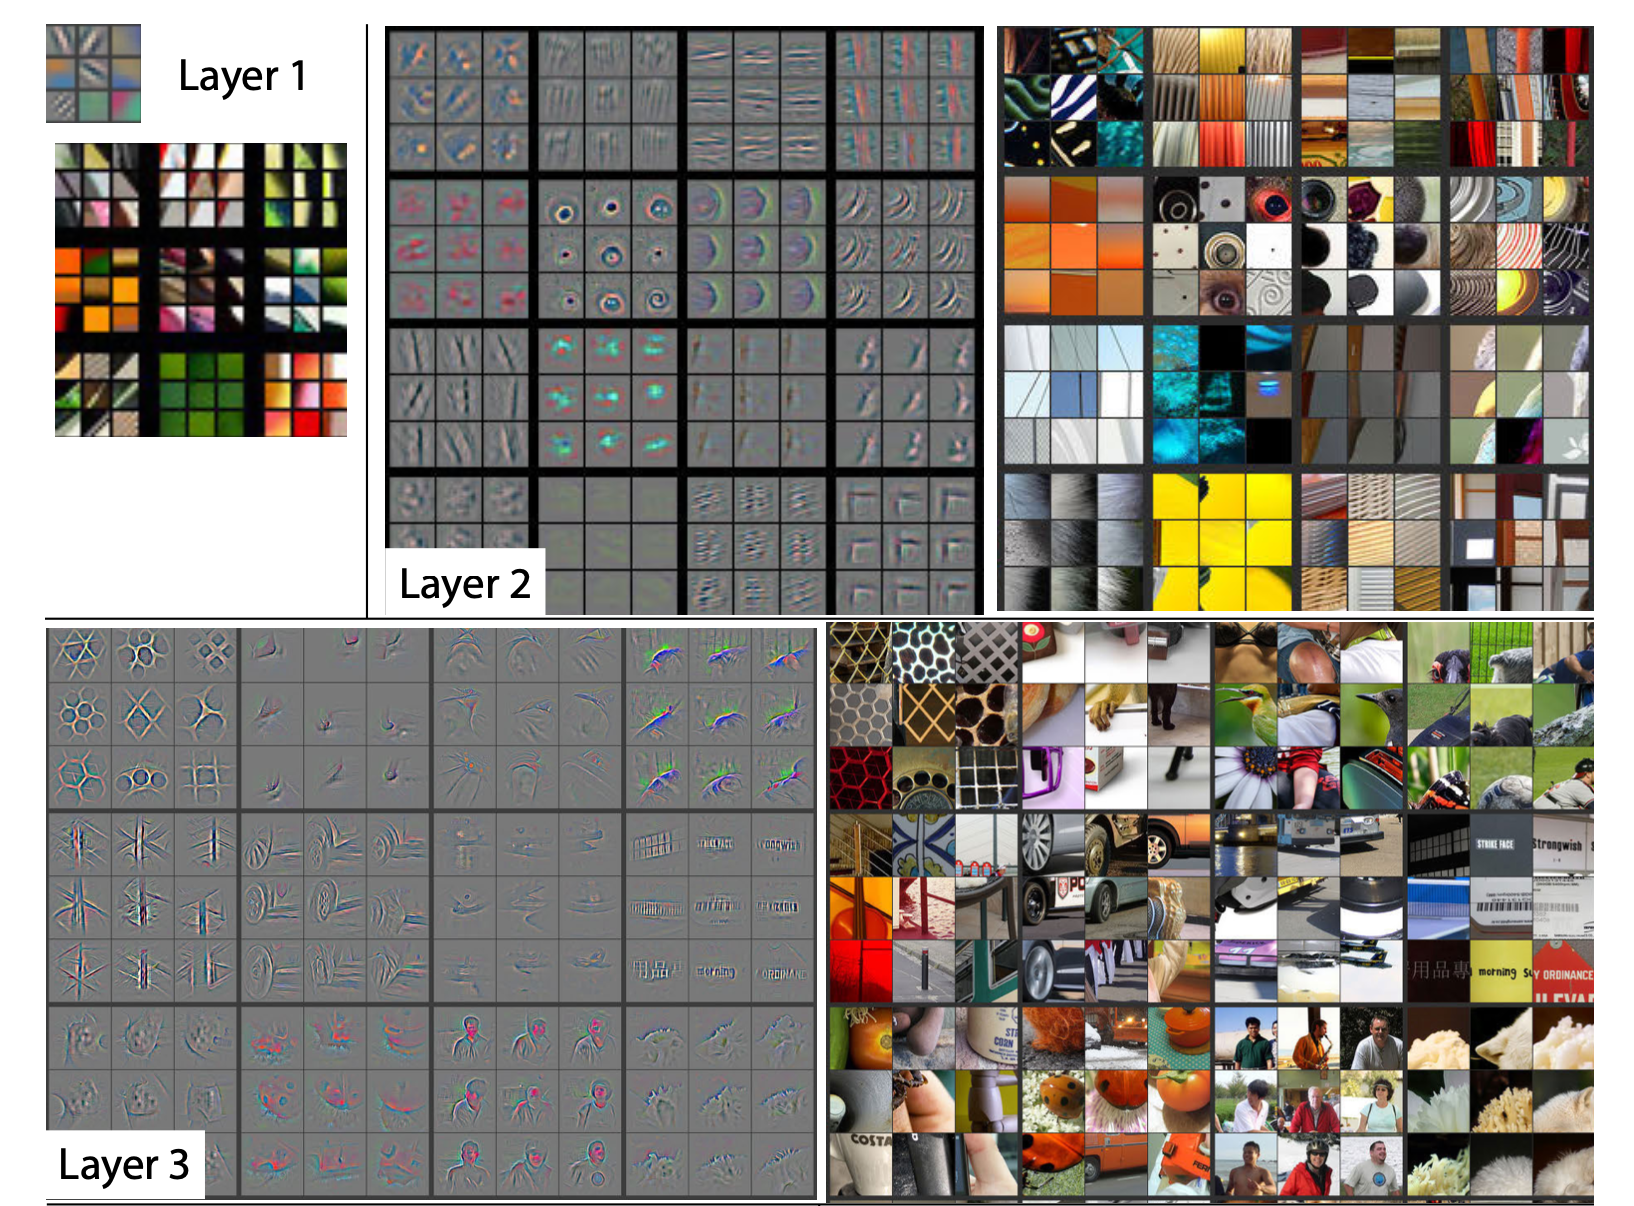
\includegraphics[width=\linewidth]{Zeiler2013-DeconvMaps.png}
    \caption{DeconvNet maps (source: \cite{Zeiler2013})}
    \label{fig:deconvnetmaps}
\end{figure}

\subsection{Saliency maps}
\cite{Erhan2009}, \cite{Simonyan2014}

Saliency map is a visualization technique using gradient-based method to observe the behavior of a deep neural network. We will tackle two different approaches :
\begin{itemize}
    \item Class model visualization
    \item Image-specific class saliency visualization
\end{itemize}  
Then, we will study the link between these techniques and the DeconvNet reconstruction.

With a class model visualization, we generate a picture representing a given class to understand the structure/behavior of it.

Formally, we want to maximize the difference between the score of a given class and our regularized picture : 
\[\arg \underset{I}{\max} {S_c(I)-\lambda{\Vert I \Vert^2}}\]

Furthermore, we use the score of the given class and not the class posterior because it is possible to maximize the previous difference discriminating others classes.

With image-specific class saliency visualization, we want to understand neural contribution/influence on the classification choice.
\begin{itemize}
    \item First, we generate a baseline typically a grey-scale image with a given class \(c\).
    \item Then, after  we find \(w\) by back-propagation.   
    \item Finally, this is how we generate the image : \(M_{(i,j)} = |w_{h(i,j,c)}|\) where \((i,j)\) is pixel position.
\end{itemize}

This method is particularly used for object location. Indeed, the magnitude of \(w\) and the picture profil are linked.

We can compare these methods to DeconvNet reconstruction which is based on back-propagation from the output of the DNN. The derivation keeps linearity and activation functions are approximated. \cite{Simonyan2014} shows that these gradient-based methods are equivalent.

\subsubsection{Enhanced saliency maps}

Images produced by back-propagation look very weird to human, they contain part of objects or artifacts that are repeated. \cite{Mahendran2015} and \cite{Nguyen2016} are making proposals to get saliency images that are more interpretable by humans. When performing the gradient maximization through back-propagation, regularizers are added to avoid high frequency pixel variations and favor the center part of the image.

Moreover, in \cite{Nguyen2016}, the baseline (called there prior) is selected in order to trigger the saliency of several facets of the target neuron. This is performed by computing the activation of many images triggering the target neuron, projecting these activations to 2D with t-SNE and then performing K-means clustering. This technique is used later in \cite{Carter2019}.

\subsection{Integrated gradients}
\cite{Sundararajan2017}

The main issue of any machine learning model is the link between the prediction and the input features. This problem is fundamental with DNN which behaves as black boxes.

\cite{Sundararajan2017} put the two following axioms to answer this problem: 
\begin{itemize}
    \item Sensitivity : \emph{"for every input and baseline that differ in one feature but have different predictions then the differing feature should be given a non-zero attribution"}
    \item Implementation invariance : \emph{"Two networks are functionally equivalent if their outputs are equal for all inputs, despite having very different implementation"}
\end{itemize}

\cite{Sundararajan2017} defines a gradient-based method respecting these two axioms : integrated gradients.

\[IntegratedGrads_i(x) = (x_i - \tilde{x_i}) \int_{\alpha=0}^{1} \frac{\partial F(\tilde{x}+\alpha x (x-\tilde{x}))}{\partial x_i} d\alpha \]

where F is a DNN, x the input et \(\tilde{x}\) the baseline. 

Integrated gradients verifies the following proposition : 

\[\sum_{i=1}^{i=n} IntegratedGrads_i(x) = F(x) - F(x) \]

This approach is interesting by the good results we obtained for instance in object location. Moreover the previous axioms help us to link the contribution of main features of DNN.

\subsection{Activation differences}
\cite{Shrikumar2017}

As for Integrated Gradients (see above), Activation differences is based on the comparison of the test image (or sample) to a baseline in order to find which pixels are the most contributing to the final classification or to any neuron unit activation.

Deep lift is designed in order to compute the \(C_{\Delta_{x_i},\Delta_{t}}\) such that:

\[ \sum_{i=1}^n C_{\Delta_{x_i},\Delta_{t}} = \Delta_t\]

It is computed through a modified chain rule of multipliers.

Let's define a multiplier on the contribution of \(\Delta_x\) to \(\Delta_t\) as : 
\(m_{\Delta_{x},\Delta_{t}} = \frac{C_{\Delta_{x_i},\Delta_{t}}}{\Delta_x} \)

The chain rule of multiplier through an hidden layer of units \(y_i\) is :

\[ m_{\Delta_{x},\Delta_{t}} = \sum_j m_{\Delta_{x},\Delta_{y_j}} m_{\Delta_{y_j},\Delta_{t}}  \]

\begin{figure}
    \centering
    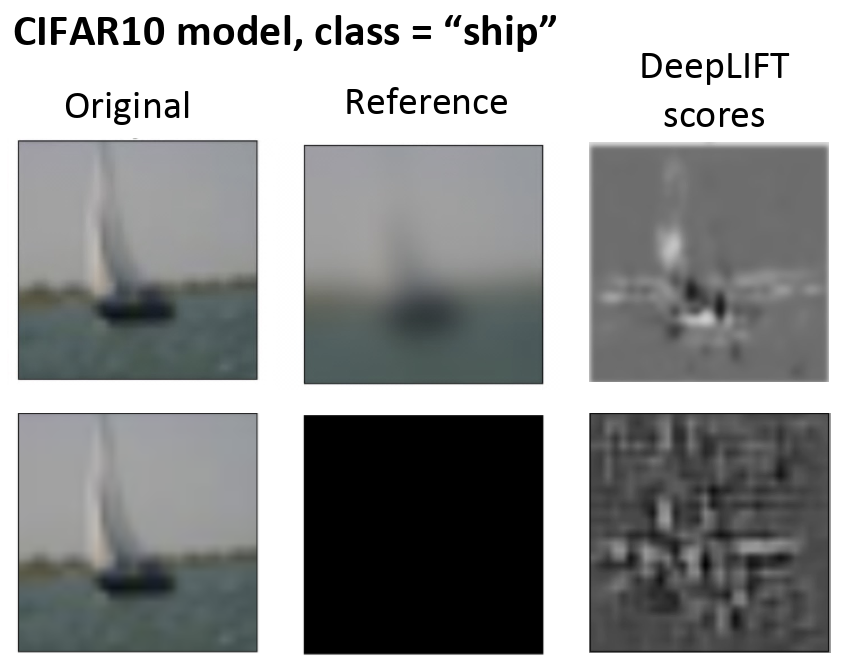
\includegraphics[scale=0.5]{Shrikumar2017-BaselineImportance.png}
    \caption{DeepLIFT on baseline (reference) importance (source: \cite{Shrikumar2017})}
    \label{fig:deeplift-baseline}
\end{figure}

One refinement of the latest paper on DeepLIFT is to separate positive and negative contributions:

\[\begin{aligned} \Delta y &=\Delta y^{+}+\Delta y^{-} \\ C_{\Delta y \Delta t} &=C_{\Delta y^{+} \Delta t}+C_{\Delta y^{-} \Delta t} \end{aligned}\]
 

\subsection{Attribution maps overview and comparison}

\cite{Ancona2018} is performing a review of all the methods explained in this section, and the Layer-wise Relevance Propagation (LRP) of \cite{Bach2015}. We have not reviewed the LRP as it is found to be close to the DeepLIFT but with more limitations.

Conclusions of this paper are:
\begin{itemize}
    \item Integrated gradients are slightly outperforming DeepLIFT since the latter does not support some products of non-linear functions (activations)
    \item All the reviewed techniques are relying on a linear approximation of the network. Their performance is optimum only in case of linear model.
\end{itemize}


\subsection{Map Atlases}

Compared to the original activation maps, saliency and attribution maps are great improvements since they map layer units back to the image space which is interpretable by a human vision. However, the complexity is still high as there are still a huge number of units to visualize and the display is based on an image or a small set if images as in \ref{fig:deconvnetmaps}.

To get a better understanding of the impact of several images and to find similarities of the attribution maps, \cite{Nguyen2016} is using t-SNE in order to group saliency maps with similarities.

\begin{figure}[H]
    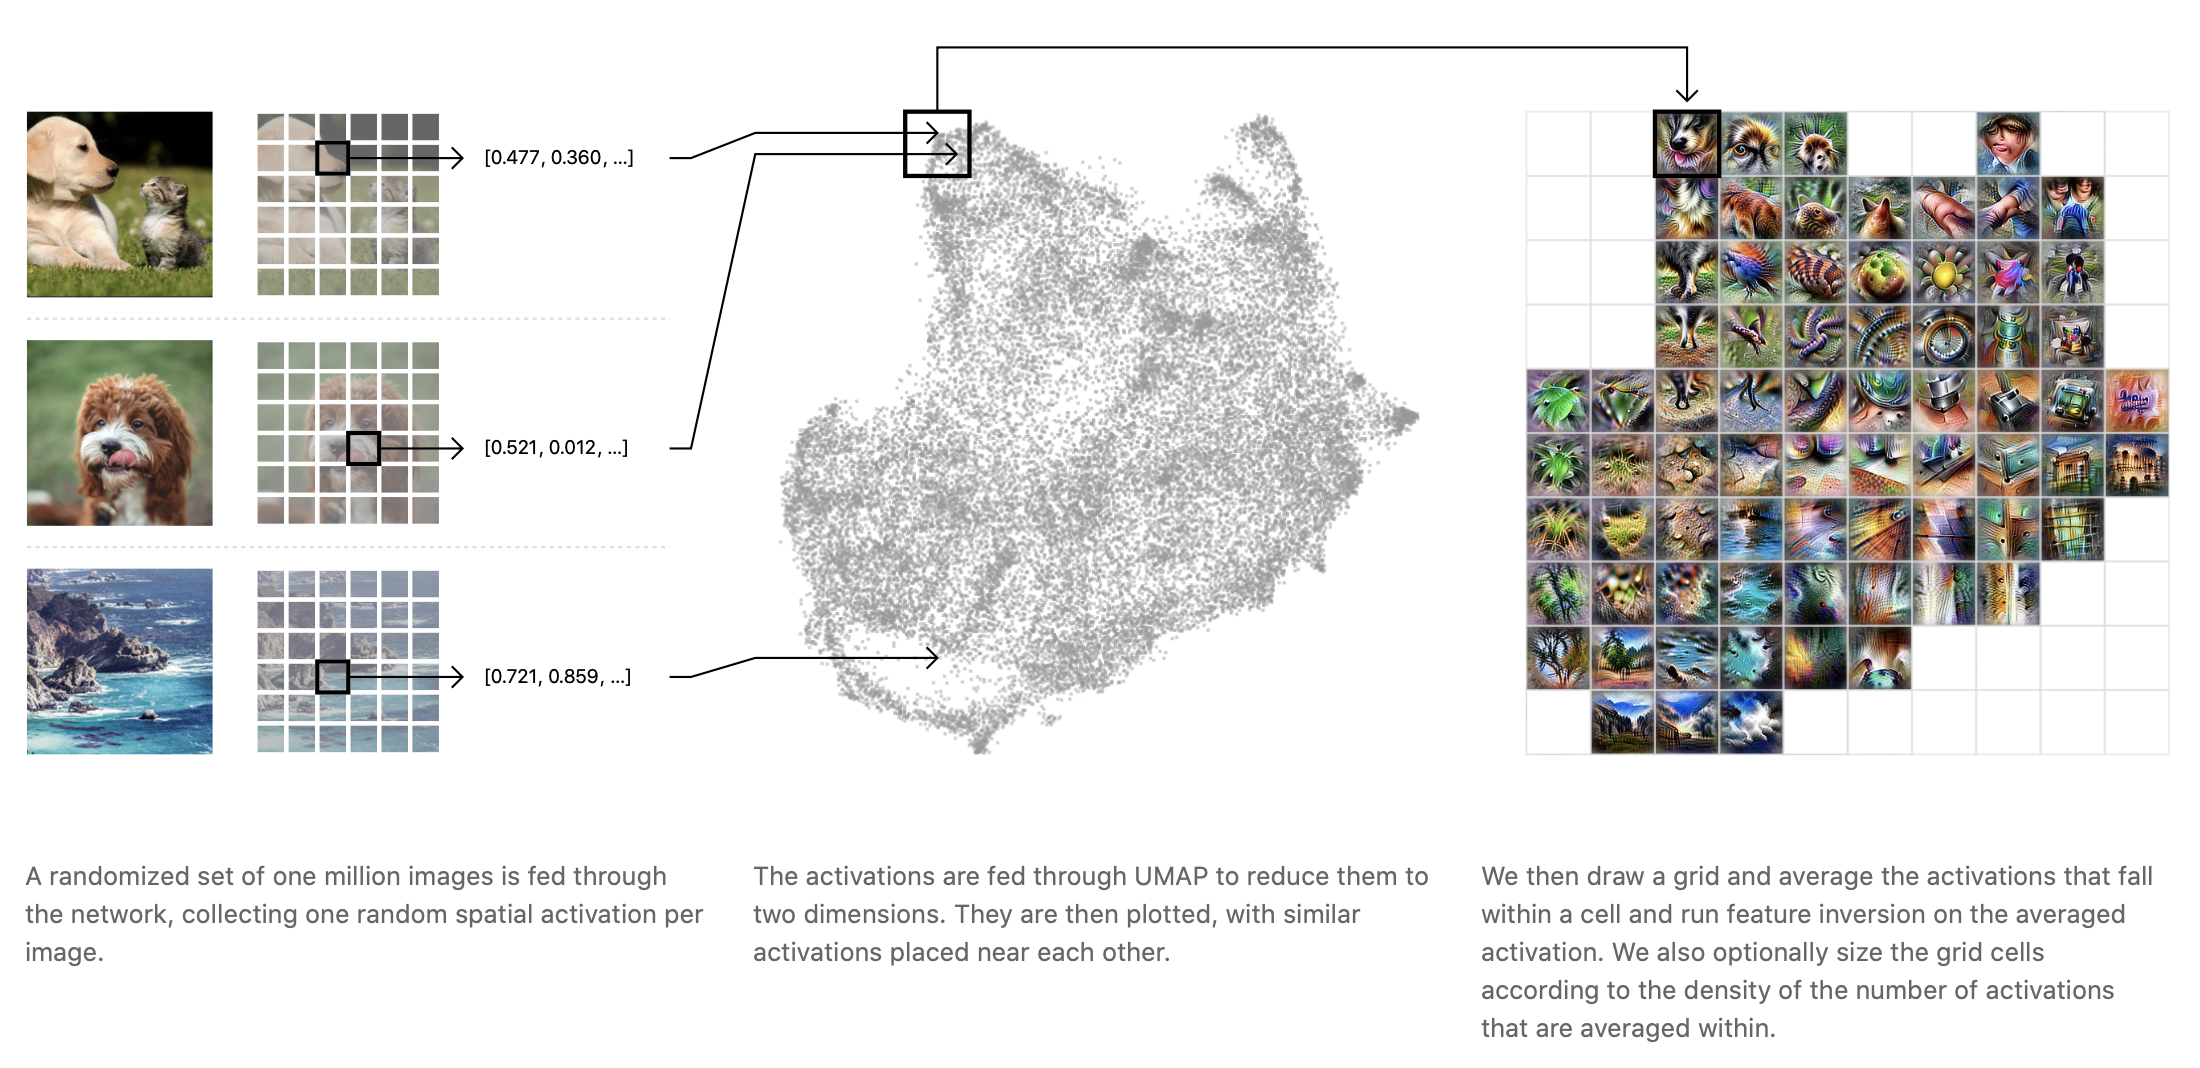
\includegraphics[width=\linewidth]{Carter2019-AtlasHow.png}
    \caption{Activation atlas \cite{Carter2019}, combination of saliency maps}
    \label{fig:atlas-how}
    \centering
\end{figure}

Activation atlases of \cite{Carter2019} goes one step further by sampling activations from many images, using t-SNE or UMAP to gather activation within the 2D plan, and averaging the saliency maps.




\newpage
\section{Adversarial attacks}
\label{sec3}

\subsection{Generating and defending against adversarial attacks}

\subsubsection{Nomenclature of attacks}

We have recently seen deep neural networks match or exceed human-level performance in otherwise arduously difficult tasks (e.g. self-driving cars, medical diagnosis, natural language processing) in the early 2010s. At the same time, there has been a growing body of research literature, starting with \cite{Szegedy2014} and \cite{Goodfellow2014}, on how deep neural networks could be crippled by external attacks designed to fool those models into making (seemingly) absurd mistakes. An early infamous example of how easy it is to cripple state-of-the-art neural networks was provided by \cite{Goodfellow2014}: the authors were able to easily fool a (then state-of-the-art) GoogleLeNet architecture into misclassifying a panda for a gibbon by introducing imperceptible pixel changes to the original image (cf. Figure \ref{fig:Adv_001_Fig}).


\vspace{0.2cm}

\begin{figure}[H]
	\centering
	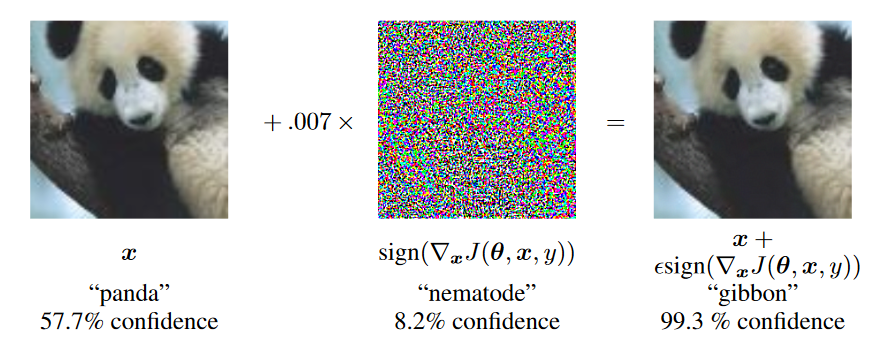
\includegraphics[scale=0.85]{images/adversarial_attacks/Adv_Fig_001_Panda_Picture.PNG}
	\caption{An example of fooling GoogleLeNet into mistaking a panda for a gibbon, source: \cite{Goodfellow2014}}
	\label{fig:Adv_001_Fig}
\end{figure}

\vspace{0.2cm}

Such vulnerabilities constitute a major roadblock for further inroads of AI-Deep Learning-based applications in more critical decision-making fields (e.g. governmental/military applications, more invasive medical procedures). This is further compounded by the ominous nature of adversarial attacks, which the research community is still debating today over its theoretical origins and whether (or not) it is specific to Deep Learning.

The possibility of crippling machine learning algorithms was already a research topic in the early 2000s. But the successes of Deep Learning have further elevated the need for researchers and industry-specialists to tackle the brittleness of machine learning algorithms when deployed outside a closed system where distributional assumptions on the data no longer hold.

As seen in \cite{Nicolae2018AdversarialRT}, there is a distinction between attacks specifically designed to fool neural networks (known as adversarial attacks) and those designed to poison the model's training set thus also crippling the predictive power of neural networks (poisoning attacks). Among adversarial attacks, there is a further demarcation between targeted attacks (where the neural network is fooled into predicting a specific class) and untargeted attacks (fooled into predicting any class). We will mainly focus on untargeted attacks for the remainder of this section. And more importantly, there is an additional distinction between white-box and black-box approaches to generating adversarial attacks.


\subsubsection{White-box and black-box methods}

Assume we are in a multi-classification setting with model image inputs $ x \in \mathbb{R}^{W \times H \times C} $ where $W$, $H$ and $C$ are respectively image width, height and the number of colour channels. The classification of an input $x$ as an output vector $y \in \mathbb{R}^K $ (where $K$ is the number of labels)  is given by a classifier $C$:

$$ C(x) = \arg \max_{y\in \{0,...,K\}} F_y (x) $$

where $F$ is a function that outputs the softmax probabilities for an input image $x$. From there, the most common approach for generating adversarial attacks to fool a specific neural network requires accessing the model's internals: notably the model's cost function $L: X \times Y \rightarrow \mathbb{R} $ such as the cross-entropy function and gradients $\nabla_x L(x,y)$. Once accessed, a wide range of techniques can be used to craft adversarial examples with relatively low complexity.

An early approach for generating adversarial attacks, still used today due to its computational efficiency, is the Fast Gradient Sign Method (FGSM). First introduced by \cite{Goodfellow2014} as a more efficient-version of \cite{Szegedy2014}, it consists in perturbing an image $x^{*}$ labelled $y^{*}$ with an imperceptible perturbation $\psi(x^{*})$. With our human vision, the newly perturbed input $x_{adv}^{*} = x^{*} + \psi(x^{*})$ is still ostensibly the same image as before. But when fed into our classifier, it ends up predicting the wrong class: $C(x^{*} + \psi(x^{*})) \neq y^{*}$. More specifically to FGSM, the adversarial perturbation $\psi(x^{*})$ is crafted by using the model's loss gradients $\nabla_{x^{*}} L(x^{*},y^{*})$ for a given image $x^{*}$:

$$ \psi(x^{*}) = - \varepsilon \cdot \mathbf{sign}(\nabla_{x^{*}} L(x^{*},y^{*})) $$

$$ x_{adv}^{*} = \mathbf{clip}(x + \psi(x^{*}), x_{min}, x_{max} )$$

where $\varepsilon$ is the strength of the attack. Excessive $\varepsilon$ values will make the adversarial attack more noticeable to human observers. The clipping function as well as input bounds $x_{min}$ and $x_{max}$ ensure that the adversarially crafted input remains an image.

There have been alternative white-box approaches for generating adversarial attacks, notably Projected Gradient Descent (PGD), Jacobian Saliency Map Attack (JSMA) or Carlini \& Wagner $L_2$ Attack (C\&W). IBM's Adversarial Robustness Toolbox from \cite{Nicolae2018AdversarialRT} has a wide range of options for crafting more sophisticated white-box adversarial attacks. Nevertheless, due to its computational efficiency, FGSM remains a popular technique for applications that require generating a large set of adversarial examples (notably adversarial training as we will see in a later subsection).

One notable weakness of white-box methods for targeting deep neural networks is that they require accessing the network's internals (notably gradients). Since \cite{Papernot2017PracticalBA}, black-box methods for fooling deep neural networks were devised, requiring neither access to the model architecture or the original training set used to train the targeted model. Examples include using substitute models mimicking the targeted classifier for crafting adversarial examples, Zeroth-Order Optimization or HopSkipJump Attack. These techniques exploit the transferability property of adversarial attacks (which will be further explored in the next section) and have shown high attack success rates against state-of-the-art architectures as seen in \cite{Papernot2017PracticalBA} and \cite{Chen2017ZOOZO}.


\subsubsection{Defences against adversarial attacks}

Machine Learning researchers have devoted a lot of time and effort on devising effective counter-measures for protecting neural networks from adversarial attacks. They broadly fall into three main categories:

\begin{itemize}
	\item \textbf{Adversarial Training}: one of the earliest defence strategies is introducing adversarial examples into the training phase, generated from the initial training data. The authors \cite{Szegedy2014} and \cite{Goodfellow2014} who brought the existence of adversarial attacks to the attention of the research community proposed adversarial training as an easily implementable approach for hardening classifiers against adversarial attacks. For generating adversarial examples, FGSM is the preferred approach due its low computational complexity.
	\item \textbf{Image Squeezing}: as detailed in \cite{Nicolae2018AdversarialRT}, there exists a number of compression techniques (such as JPEG or thermometer compression) for blurring images, therefore reducing the magnitude of adversarial perturbations. \cite{Shafahi2018} provides a theoretical justification in that blurring images reduces image complexity thus leading to a classifier with a more concentrated image distribution making it more robustness to attacks.
	\item \textbf{Anomaly Detection}: this approach augments the existing classifier to help detect whether an incoming image is an adversarial example or not. One of the more complex attempts from \cite{Samangouei2018DefenseGANPC} to dampen the magnitude of adversarial attacks is to "project" input images into a separately-trained Generative Adversarial Network (GAN) and feed the GAN's output into the classifier rather than the original image.
\end{itemize}


Despite the proliferation of defensive strategies, as pointed out by \cite{Shafahi2018}, many of those techniques have almost been immediately broken. Most of these approaches are only suited for shielding neural networks against a specific type of attack (e.g. white-box, black-box), e.g. adversarial training with FGSM can be easily circumvented with more advanced black-box attacks.



\subsection{Why study adversarial attacks?}

\subsubsection{Existence and transferability of adversarial attacks}

The existence and inevitability of adversarial attacks have been a major research topic within the Machine Learning research community since \cite{Szegedy2014} and \cite{Goodfellow2014}.

One of the earliest explanations for the puzzling behaviour of adversarial attacks was provided by \cite{Goodfellow2014} as the "linear hypothesis". Suppose we start in the linear case and we make small additive perturbations to an input image such that $\tilde x = x + \eta $, our classifier will yield the following output:

$$ w^T \tilde x = w^T x + w^T \eta $$

If this additive perturbation is small enough, where $\Vert \eta \Vert_{\infty} \leq \epsilon$, then it would not make sense for the classifier to react differently (i.e. predict a different label). We can see that there is a linear relationship between our perturbation and its effect on our classifier $ w^T \eta $.

But as \cite{Goodfellow2014} points out, increasing the complexity of the images we are dealing with (e.g. moving from greyscale to RGB) also simultaneously increases (linearly) the damage those perturbations can wreck on our classifier. This comes from the fact that the more complex our image becomes, more and more pixels become available to be fooled around. Thus, it becomes easier to make imperceptible input changes on larger swaths of our image (such that the image still looks broadly the same as before since $\Vert \eta \Vert_{\infty} \leq \epsilon$). The  higher the dimensionality of our targeted image is, the more potent the perturbations $ w^T \eta $ will be on our classifier. While this explanation was elaborated for linear models, \cite{Goodfellow2014} claims that this also holds true for neural networks. Neural networks in multi-class classification by construction use softmax regression for making predictions, which is in itself a generalization of logistic regression - a linear model.


The high-dimensionality of images has thus been the preferred explanation for the continued existence of adversarial attacks. As pointed out by \cite{shafahi2018adversarial}, many studies have shown that state-of-the-art neural networks are more easily fooled on RGB datasets (e.g. CIFAR-10, ImageNet) than on grey scaled datasets (e.g. MNIST).

While there have been numerous hints that the high-dimensionality of RGB image datasets might be the root cause of adversarial attacks, \cite{shafahi2018adversarial} have shown that dimensionality is not necessarily by itself the main driver behind the ease of crafting attacks to fool neural networks or even the failure of many adversarial defensive strategies. They created an upscaled version of MNIST with higher resolution grey scaled images of shape $56 \times 56$ ($b$-MNIST) and test the robustness of different neural networks on MNIST, $b$-MNIST and CIFAR-10. Even though $b$-MNIST roughly has the same pixel complexity as CIFAR-10, the adversarial robustness on $b$-MNIST is roughly the same as with MNIST thus noticeably higher than with CIFAR-10 models.


For the authors, input concentration - specifically how diversely distributed the images are in input space - is likely to play a more important role than dimensionality alone. This ties smoothly with their finding that the success rate of adversarial attacks stems primarily from how concentrated the input image space is: classifiers trained on highly-concentrated image data will be more robustness to adversarial attacks. The MNIST dataset is highly concentrated since images tend to roughly have the same profile: centred grey-scaled digits. Thus, upscaling MNIST wouldn't lead to changes in input image distribution thus adversarial robustness would not change in anyway. Conversely, CIFAR-10 has lower data concentration due to higher image complexity. Theoretically, this should increase the successfulness of adversarial attacks (which is confirmed in the case of MNIST-trained classifiers being more adversarially robust than CIFAR-10 or ImageNet classfiers).


Another intriguing property of adversarial examples is their transferability. \cite{moosavidezfooli2016universal} showed a rather disconcerting result. It is possible for a specific neural architecture (e.g. VGG16, Inception, ResNet) to craft model-specific perturbations that will succeed in defeating the said architecture all the time, regardless of the dataset. They have even shown these examples can also transfer between model architectures. These are known as universal adversarial attacks.



\vspace{0.2cm}

\begin{figure}[H]
	\centering
	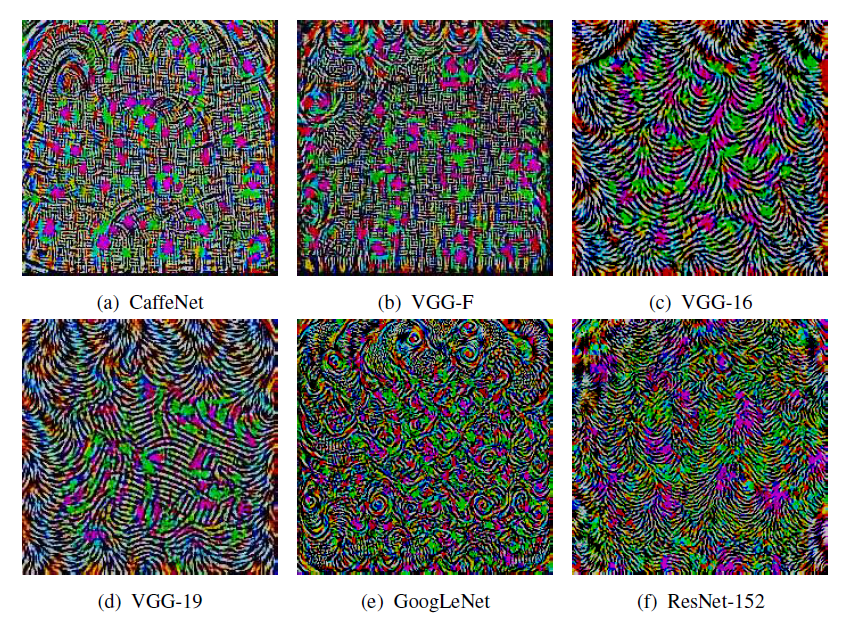
\includegraphics[scale=0.85]{images/adversarial_attacks/Adv_Fig_002_UAE.PNG}
	\caption{Universal adversarial attacks for different state-of-the-art classifiers, source: \cite{moosavidezfooli2016universal}}
	\label{fig:Adv_002_Fig}
\end{figure}

\vspace{0.2cm}


\subsubsection{Vulnerabilities in real-world conditions}

Even though adversarial attacks have bore the focus of the research community since the 2010s, there exists another type of vulnerability that has seen less attention but is likely to happen more often than not in a real-world environment: corruption robustness (e.g. brightness changes, blur, pixelation, anomalous objects disrupting images, random rotations). According to \cite{ford2019adversarial}, at first adversarial attacks and corruption vulnerabilities are seemly unrelated, but in reality it turns out to be opposite.

\vspace{0.2cm}


\begin{figure}[H]
	\centering
	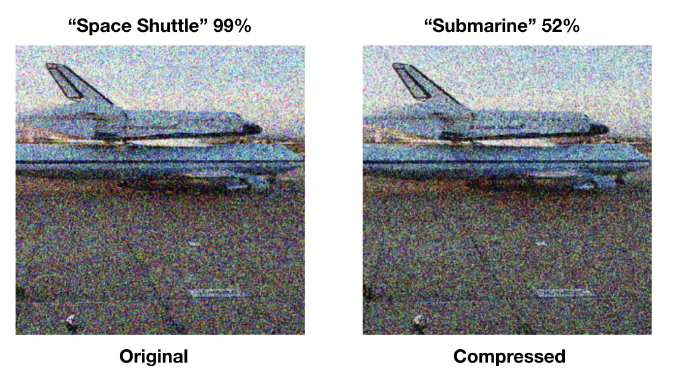
\includegraphics[scale=0.85]{images/adversarial_attacks/Adv_Fig_003_Gaussian_Noise.PNG}
	\caption{Corruption robustness on ImageNet after adding Gaussian noise, source: \cite{ford2019adversarial}}
	\label{fig:Adv_003_Fig}
\end{figure}

\vspace{0.2cm}

\cite{ford2019adversarial} show (theoretically) on linear models that adversarially generated examples lie on the same high dimensional image space as images generated with additive Gaussian random perturbations. They extend their initial results to neural networks by running a number of experiments on CIFAR-10 and ImageNet. From a distributional perspective, adversarial attacks and corruption vulnerabilities emanate from the same underlying manifold.

Self-driving cars are an example of a field where the consequences of adversarial attacks could be particularly severe. While brittleness to blurred/corrupted video planes is most likely to be the most obvious threat for self-driving cars, \cite{Ranjan2019AttackingOF} have shown that targeted attacks (e.g. adversarial image patches that amount to less than 1\% of the total video frame) can compromise video streams and consequently self-driving cars.

\vspace{0.2cm}


\begin{figure}[H]
	\centering
	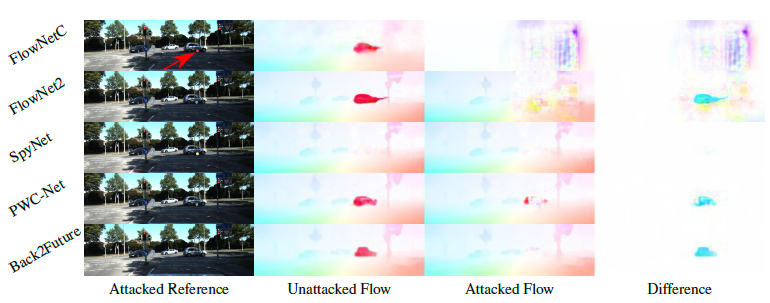
\includegraphics[scale=0.94]{images/adversarial_attacks/Adv_Fig_004_Self_Driving_Cars.PNG}
	\caption{Adversarial patches on video streams, source: \cite{Ranjan2019AttackingOF}}
	\label{fig:Adv_004_Fig}
\end{figure}

\vspace{0.2cm}

Another novel playground for adversarial attacks is fooling deepfake detectors. Concern over the dangerousness of deepfakes in spreading disinformation has led tech giants such as Facebook and Twitter to develop deepfake detectors. In February 2020, Kaggle even hosted a DeepFake detection competition with the blessing of major tech companies such as Amazon, Microsoft and Facebook. But more recent studies from \cite{Neekhara2020AdversarialDE} and \cite{Gandhi2020AdversarialPF} have shown that deepfake detectors can be easily fooled by even the simplest methods such as FGSM.


\subsubsection{Is there a trade-off between robustness and generalization?}

A more pressing concern is whether improving the robustness of classifiers against adversarial attacks necessarily leads to a trade-off in performance. Popular adversarial defences such as adversarial training introduce adversarially generated examples during backpropagation, which could theoretically diminish predictive performance on newer images.

\cite{tsipras2018robustness} found that there exists effectively an empirically-observable trade-off between robustness to adversarial attacks and testing set performance as seen on Figure \ref{fig:Adv_005_Fig}. The drop in performance is slightly more pronounced on CIFAR-10.

\vspace{0.2cm}

\begin{figure}[H]
	\centering
	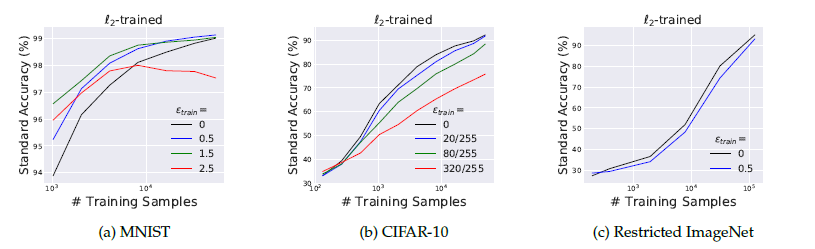
\includegraphics[scale=1.0]{images/adversarial_attacks/Adv_Fig_005_Robustness_1.PNG}
	\caption{Trade-off between adversarial robustness and testing set accuracy on adversarially trained classifiers, source: \cite{tsipras2018robustness}}
	\label{fig:Adv_005_Fig}
\end{figure}

\vspace{0.2cm}

Yet in spite of this empirical trade-off, they found that there was an unexpected silver lining in adversarially training neural networks: they ran a number of interpretability diagnostics with saliency maps in order to understand the decision-making process of neural networks (as showcased on Figure \ref{fig:Adv_006_Fig}). They found that adversarially trained neural networks did a much better job in localizing the relevant object compared to standard non-robust neural networks and thus were more semantically aligned with our human visual stream than the latter.


\vspace{0.2cm}

\begin{figure}[H]
	\centering
	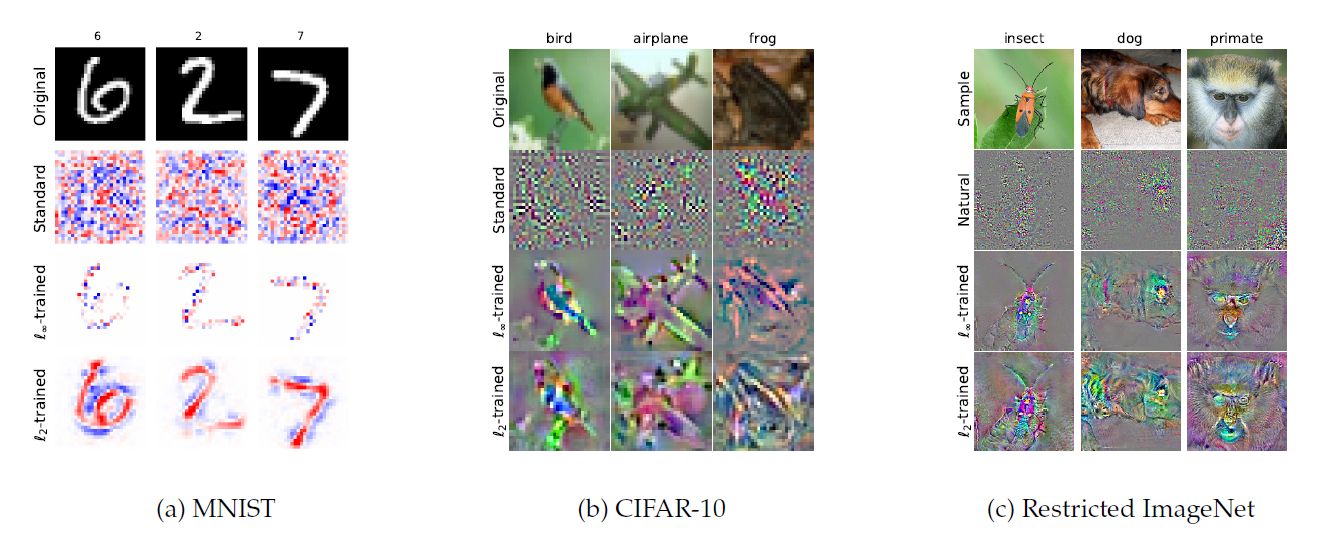
\includegraphics[scale=0.6]{images/adversarial_attacks/Adv_Fig_006_Robustness_2.PNG}
	\caption{Saliency maps on non-robust and $L_2$-adversarially trained neural networks, source: \cite{tsipras2018robustness}}
	\label{fig:Adv_006_Fig}
\end{figure}

\vspace{0.2cm}

Therefore, adversarial robustness improves model interpretability and brings black-box neural networks closer to human vision. Notably, by preventing the latter from concentrating undue attention on non-robust features and instead focus on the image contours/ensembles that would really matter when attempting to localize objects on an image.

\subsection{Adversarial robustness simulator with Plotly Dash}

To illustrate our literature review, we developed an adversarial attack simulator for stress testing Keras models. It is actually a sub-component of much larger interpretability framework - \textbf{Deep Embedding Viewer} - that we will go into greater detail later.

After selecting an available Keras model, the user can run a series of adversarial pertrubations to stress test the model's adversarial robustness. For this application, we chose to generate adversarial attacks with the FGSM method due to its low complexity and our need to generate many adversarial samples.

Once the "Run Stress Test" switch is pressed, FGSM perturbations are added to the classifier's validation/testing set. Different perturbations levels $\varepsilon$ are considered from 0.5\% to 10\%: in an ideal outcome, our neural network should be robust to attacks with low perturbation levels (e.g. 0.5\%, 1\% and 2.5\%) as at this stage the perturbations are imperceptible to an human observer.

We demonstrate the use of our simulator on a VGG-16 model trained on CIFAR-10 and evaluated on a validation set of 10,000 images. Once the simulation generated 10,000 adversarial images a performance chart is displayed (on the left in Figure \ref{fig:Adv_007_Fig}), summarizing the adversarial robustness of our classifier against different perturbation scenarios. On the right, a slider is provided to visualize concretely different perturbation $\varepsilon$ values and help the user get a better sense of how adversarial attacks discretely distort images.


\vspace{0.2cm}

\begin{figure}[H]
	\centering
	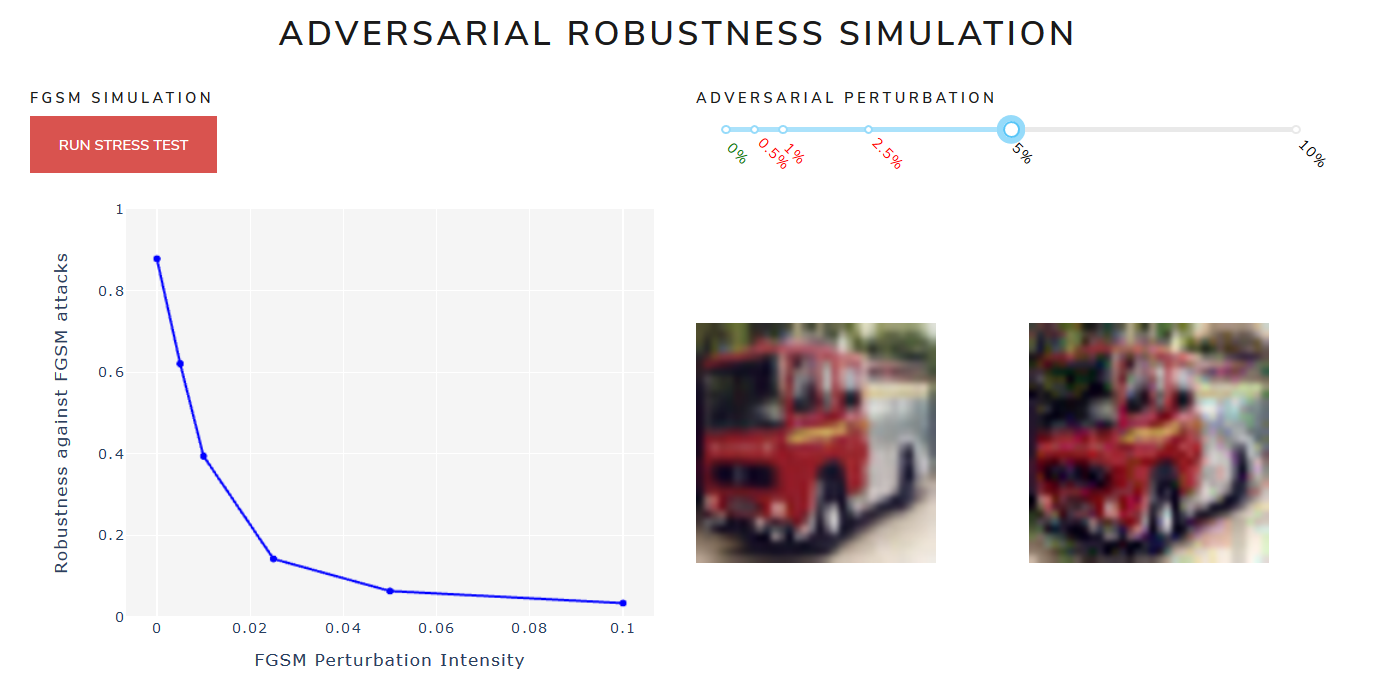
\includegraphics[scale=0.65]{images/adversarial_attacks/Adv_Fig_007_Simulator.PNG}
	\caption{Adversarial Robustness Simulator (with FGSM) for Keras Models}
	\label{fig:Adv_007_Fig}
\end{figure}

\vspace{0.2cm}



\newpage
\section{Further directions for the project}
\label{sec4}


\subsection{Simple visualization methods}
\label{subsec41}

Sections \ref{sec2} and \ref{sec3} are dealing with interpretability topics that attracted much attention in recent research. Most of these methodologies use fairly sophisticated mathematical methods, and provide beautiful representations of neural networks and their activations. One particularly representative example of such methodology is the activation atlas methodology proposed by \cite{Carter2019}.

This method is sampling activations form many images, then summarizes the activations on the 2-D plan by using a reduction dimension of t-SNE or UMAP type, and averages over the saliency maps.

Figure \ref{im_sec4_1} provides an example of activation atlas :

\begin{figure}[H]
	\centering
	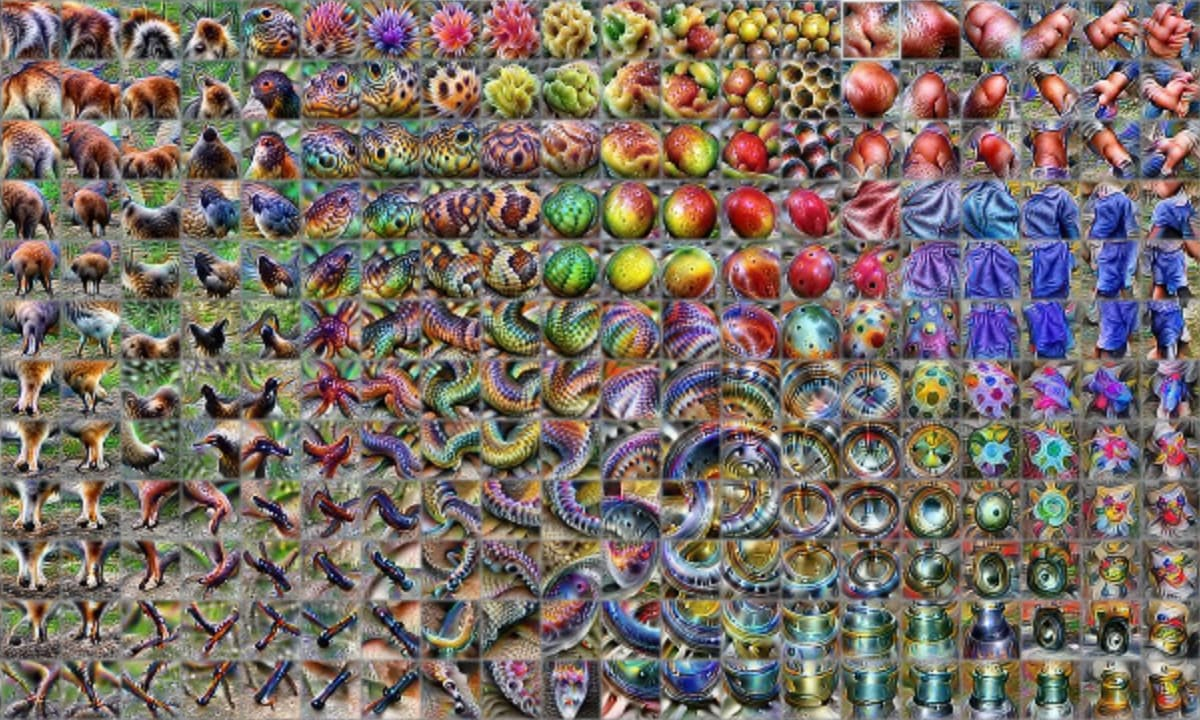
\includegraphics[width=\linewidth]{images/image2.png}
	\caption{An example of activation atlas}
	\label{im_sec4_1}
\end{figure}

While aesthetic, this representation may suffer from interpretation issues. Even though the goal of such methods is to render the network more interpretable, it is in fact quite difficult to conclude anything from such figure. To get more insights, one would need to read the paper carefully before and then look at the picture in much details to obtain useful information. For a professional with limited knowledge in neural networks, this sort of tools is probably not ideal.

On the other hand, simpler tools are being proposed in the recent literature. For instance, \cite{Peters2018} propose a more intuitive visualization method, specifically suitable for non-expert users. The method consists in representing neuron activation on a 2-D plan from a UMAP dimension reduction. In this respect, it is not so different in essence from the activation atlas. Yet the representation it provides is considerably simpler. Figure \ref{im_sec4_2} provides an example of this intuitive representation:

\begin{figure}[H]
	\centering
	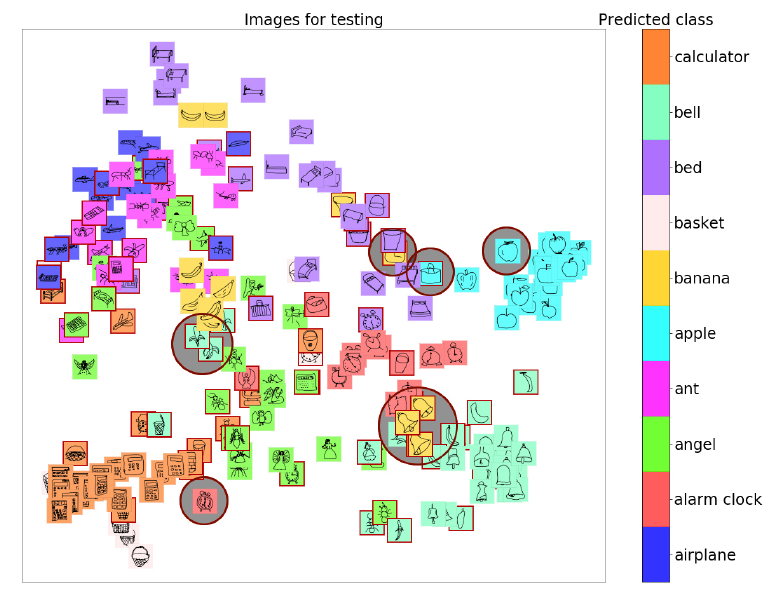
\includegraphics[width=\linewidth]{images/image5.png}
	\caption{An example of intuitive visualization}
	\label{im_sec4_2}
\end{figure}

The figure clearly discriminates the different classification categories using a palette of colors. Clustering highlights clearly which images are considered similar by the network, and miss-classified images are circled in red for immediate detection. This kind of representation does provide effective interpretation. Consider for instance the cluster of three bells on the lower-right side of the figure. These bells have been incorrectly classified as bananas, most likely because their diagonal orientation makes them closer to the other bananas than to their bell counterparts which can be seen to be in straight position.

In the end, when wondering which approach is the most informative, the second one would most likely be retained. This led our group to a real interrogation: what is the target audience for our visualization project? And what is the most suitable methodology to adopt to satisfy the needs of this audience? Should we adopt a sophisticated, state-of-the-art approach that may lead to technical performances and beautiful representations, or should we focus on simpler strategies that may in the end carry more immediate explanatory power? At the moment, we may be rather inclined to select the second solution, but this is yet a discussion to be pursued further.


\subsection{Future directions with the Minister of Armies}
\label{subsec42}

After discussion with the Ministère des Armées, we have decided to focus on the behavior of the neural network during the training. The adversarial training have been given up for our use case.
Our partner is willing to visualize how we could monitor the training through several metrics. We will deepen and extend all gradient-based and attribution technics for instance though the following metrics.
We have decided to proceeded along two mains axis :

Define following metrics : 
\begin{enumerate}
	\item Accuracy/loss during training and testing phasis, \cite{Glorot2010}, \cite{Li2017} 
	\item Evolution of gradients/weights for each epoch: cumulative differentiation between epochs to highlight DNN behavior and its main patterns, \cite{Chen2018}, \cite{Yosinski2015},  \cite{Rauber2016}, \cite{Cashman2019}
	\item Dynamic visualization of activations to observe the neural behavior and find neurons with similar or anti-similar behavior, \cite{Chen2018}, \cite{Yosinski2015}, \cite{Carter2019}
	\item Visualize the clustering evolution of main classes thanks to t-SNE or UMAP, \cite{Rauber2016} 
	\item Class discriminant features. \cite{Zintgraf2017}
	\item Provide an online tool to inspect the evolution of the deep neural network over epochs and given input samples.
\end{enumerate}

The final aim is to provide a proof of concept of some tools featuring different views based on previously listed metrics.  


\newpage

\section{Deep Embedding Visualization}
\label{sec5}

\subsection{Theoretical motivations}

\subsubsection{From occlusion maps to visualizing embeddings}

While attributions methods (e.g. Saliency Maps, Occlusion Maps, LRP, DeepLIFT, Grad-CAM) have shown promising results for decoding individual predictions and identifying "Clever Hans" correlations thus improving the transparency of deep convolutional neural networks (DCNN), scaling such methods on large-scale datasets would unrealistically require a human operator to process tens of thousands of heatmaps as shown in \cite{Lapuschkin_2019}.

A more comprehensive visualization framework for Explainable AI would require complementing attribution methods with more holistic approaches in order to get a sense of how DCNNs internally assimilate and understand the input data its fed with. More specifically and following \cite{Rauber2017VisualizingTH}, we wish to monitor how well DCNNs perform the subsequent tasks:

\begin{itemize}
	\item \textbf{T1}: \textbf{Class Discrimination}. As we are in a multi-class classification setting, we wish to assess how well DCNNs are able to successfully disentangle labels from an originally messy input data space as shown in \cite{Rauber2017VisualizingTH} and understand prediction failure such as DCNNs on the ImageNet Dataset struggling to distinguish "missiles" from "projectiles" (as shown in Figure \ref{fig:HRV_001_Class_Hiearchy}) due to redundancies between both target labels as seen in \cite{Alsallakh2017Hierarchy}.
	
	\vspace{0.4cm}
	
	\begin{figure}[H]
		\centering
		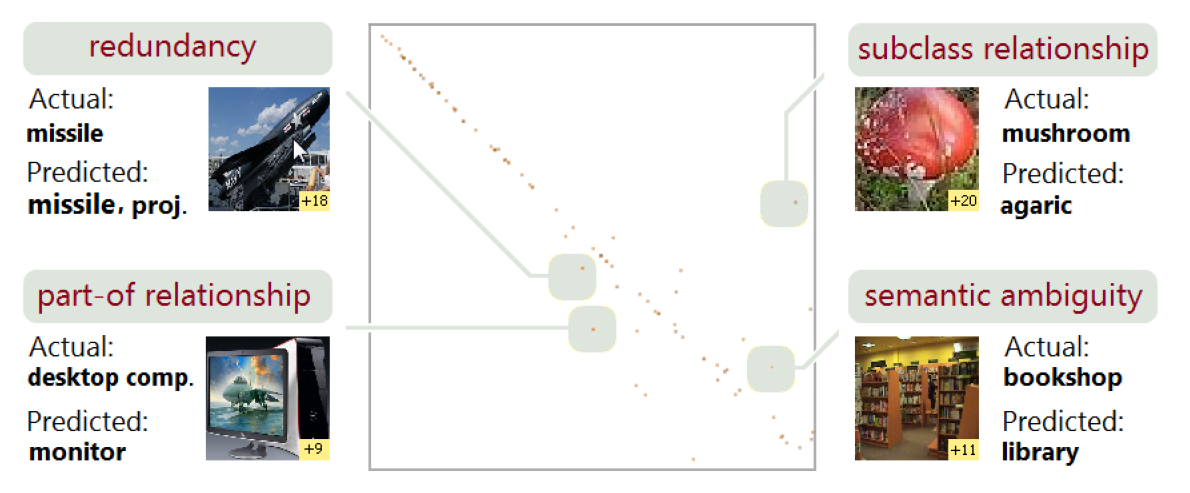
\includegraphics[scale=0.5]{images/embedding_view/HRV_Fig_001_Class_Hiearchy.PNG}
		\caption{Class confusion on ImageNet, source: \cite{Alsallakh2017Hierarchy}}
		\label{fig:HRV_001_Class_Hiearchy}
	\end{figure}
	
	\vspace{0.1cm}
	
	\item \textbf{T2}: \textbf{Neuron/Convolutional Filter Specialization}. Although state-of-the-art Deep Learning models favour overparameterization, awareness in how thousands of neurons/filters behave over differing labels as studied in \cite{Rauber2017VisualizingTH} and the existence (or not) of dead regions as highlighted by \cite{Pezzotti2018DeepEyesPV} is of keen importance for model designers.
\end{itemize}

In this regard, we found Embedding Visualization to be a suitable method for monitoring \textbf{T1} and \textbf{T2}. From \cite{Smilkov2016EmbeddingPI}, an embedding can be defined as a "map from input data to points in Euclidean space". One key strength of embeddings is that they can be used to map any given input (e.g. images, text, audio, categorical variables, graphs) into high-dimensional vectors, which can then be seamlessly projected in 2D or 3D space for user visualization with the help of dimensionality reduction methods (e.g. PCA, t-SNE, UMAP).

\subsubsection{Embeddings}

As stated by \cite{Smilkov2016EmbeddingPI}, machine learning algorithms relying on embeddings for encoding the concept of similarity between observations can be made visually accessible and easily interpretable by simply inspecting embeddings for scrutinizing and interpreting model behaviour, namely "local neighbourhoods" (how does our model perceive similar looking images?), "global geometry" (how are similarly looking image clusters interconnected with each other?) and "meaningful directions" (can we identify the latent variables driving our data?).

As an illustration, suppose a machine learning researcher develops a content-based music recommender system where music bands are encoded as high-dimensional vectors of identical shape (embeddings). A well-performing recommender system should be able to understand that Heavy Metal bands Iron Maiden and Judas Priest would have similar embeddings. It should also be able to understand in Euclidean sense how Heavy Metal bands would be much closer to Hard Rock bands than Folk or R\&B.

Widespread in Natural Language Processing for encoding word similarity (e.g. Word Embeddings and Transformers such as Word2Vec, Glove, BERT, XLNET), the concept of embeddings can also be extended to computer vision and DCNNs for encoding image similarity.

As shown on Figure \ref{fig:HRV_003_Mallat_CNN}, DCNNs are essentially functions that send their input data into a series of nonlinear convolutional operators (outputting hidden layer activations), progressively linearising the original input data to a more lower-dimensional manifold where the labels are more easily separable (through linear classifiers). This is akin to kernel methods that map nonlinear input spaces into linearly separable RKHS (albeit higher-dimensional). The difference here is that the outputs of each and every one of those intermediate convolutional operators (i.e. hidden layer activations) can be extracted as high-dimensional vectors.

\vspace{0.2cm}

\begin{figure}[H]
\centering
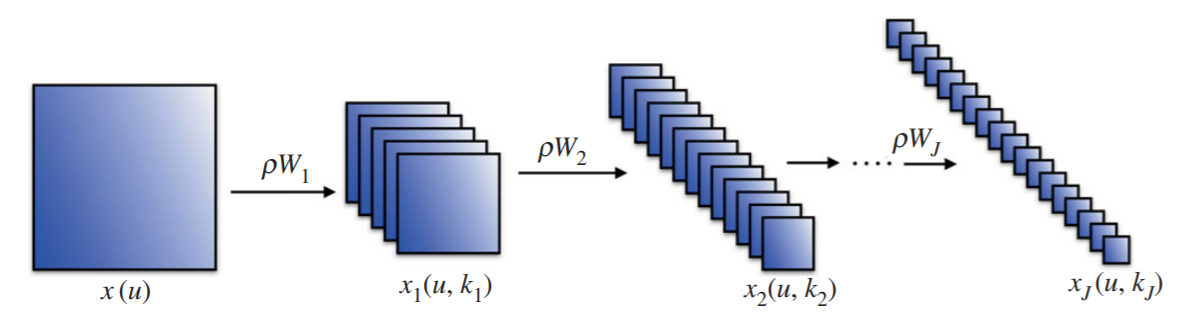
\includegraphics[scale=0.6]{images/embedding_view/HRV_Fig_003_Mallat_CNN.PNG}
\caption{A convolutional neural network: a sequence of nonlinear convolutional transformations, source: \cite{Mallat2016UnderstandingDC}}
\label{fig:HRV_003_Mallat_CNN}
\end{figure}

\vspace{0.2cm}

Thus, as pointed out by \cite{Hohman2019VisualAI}, the hidden layers of DCNNs (and by extension all Deep Learning architectures) can be viewed as embeddings (which we will then on denote as neural embeddings). This interpretation of hidden layers as embeddings has powerful implications: machine learning researchers can access those hidden layer activations as high-dimensional vectors and then visually assess them through dimensionality reduction on a 2D or 3D scatterplot. Nearly analogous to the music band recommendation example, a well-performing DCNN (as shown on Figure \ref{fig:HRV_002_Embedding_View}) should be able to perceive images from different dog breeds as having similar embeddings (i.e. images close in Euclidean space) and dog breed images as having highly dissimilar embeddings to those from ocean promontories.

\vspace{0.2cm}

\begin{figure}[H]
	\centering
	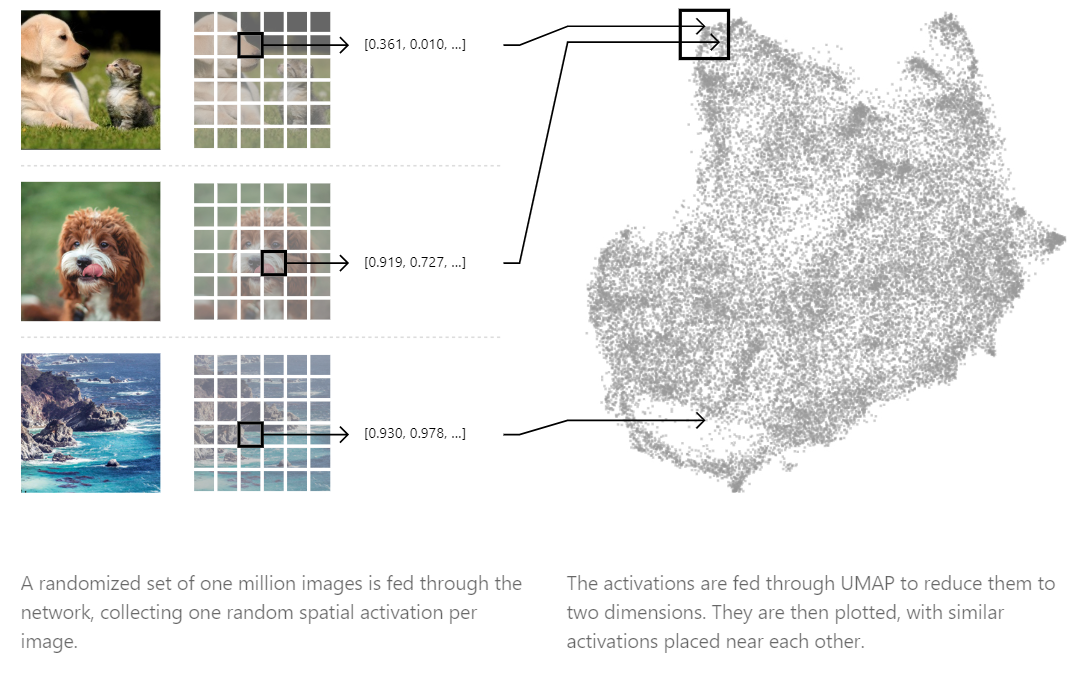
\includegraphics[scale=0.7]{images/embedding_view/HRV_Fig_002_Embedding_View.PNG}
	\caption{Randomly sampled hidden activations from InceptionV1 (mixed4c layer) projected into 2D with UMAP, source: \cite{Carter2019}}
	\label{fig:HRV_002_Embedding_View}
\end{figure}

\vspace{0.2cm}

A number of research papers across different Computer Vision fields have utilized embedding visualisation for illustrating experimental results including but not limited to:

\begin{itemize}
	\item \textbf{Deep Reinforcement Learning}: \cite{Zahavy2016GrayingTB}
	\item \textbf{Domain Adaptation}: \cite{ganin2015domainadversarial}, \cite{Sener2016LearningTR}, \cite{Li2017RevisitingBN}; \cite{Li2018ExtractingRB}
	\item \textbf{Adversarial Robustness Training}: \cite{Chen2019ImprovingAR}; \cite{Mustafa2019AdversarialDB}
	\item \textbf{Deep Metric Learning}: \cite{Song2016DeepML}; \cite{Wang2017DeepML}
\end{itemize}

A number of open-source and in-house visual analytics software also use embedding display as a major feature of their visualization framework:

\begin{itemize}
	\item \textbf{Embedding Projector (Tensorboard)}: \cite{Smilkov2016EmbeddingPI}
	\item \textbf{RevaCNN}: \cite{ChungReVACNN2016}
	\item \textbf{ActiViz (Facebook)}: \cite{Kahng2018ActiVisVE}
	\item \textbf{DeepEyes}: \cite{Pezzotti2018DeepEyesPV}
	\item \textbf{TopoAct}: \cite{Rathore2019TopoActET}
	\item \textbf{Summit}: \cite{hohman2020summit}
\end{itemize}

Embedding visualization sits nicely with recent work on biological interpretations of how DCNNs operate and the need for deeper architectures. As detailed in \cite{Mallat2016UnderstandingDC}, DCNNs subjects its input image data to a series of linear operations through convolutional filters followed by nonlinear transformations through activation functions. Such operations help further linearise an initially high-dimensional input space ($\mathbb{R}^{3072}$ on CIFAR-10 and $\mathbb{R}^{196608}$ on ImageNet) such that at the end of our sequence, the newly linearised input data can easily be separated with a linear classifier (e.g. logistic/softmax classifier). This linearisation capacity has seen interesting analogies with the primate visual cortex's ability of progressively flattening high-dimensional object manifolds such that the brain can easily discriminate between objects, as seen in \cite{DiCarlo2007UntanglingIO} and \cite{Cohen2020SeparabilityAG}. The brain's faculty of easily discerning objects from originally intricate images has even been represented as a linear hyperplane separator as seen in Figure \ref{fig:HRV_004_Cortex_View}.

\vspace{0.2cm}

\begin{figure}[H]
	\centering
	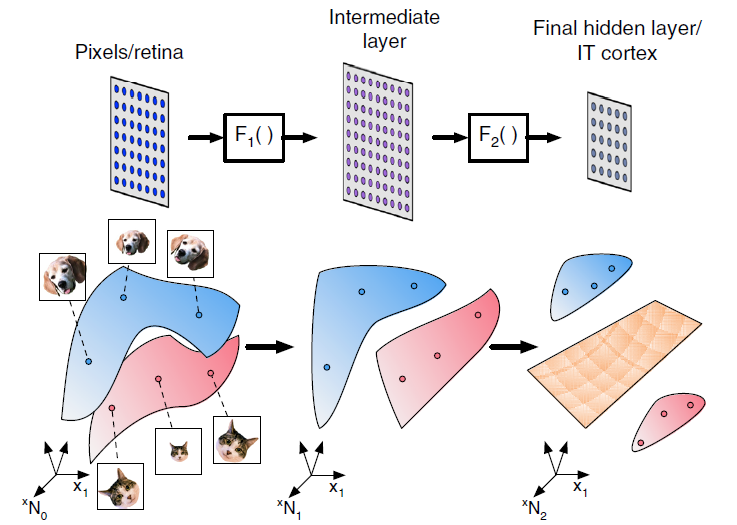
\includegraphics[scale=0.8]{images/embedding_view/HRV_Fig_004_Visual_Cortex.PNG}
	\caption{Linearisation of high-dimensional object manifolds (labelled input images) with DCNNs, source: \cite{Cohen2020SeparabilityAG}}
	\label{fig:HRV_004_Cortex_View}
\end{figure}

\vspace{0.2cm}

This gives us a useful heuristic for monitoring the convolutional layers' internal behaviour: the more visually separated the embeddings in 2D space are, the likelier we can posit that our DCNN is capable of discriminating the classes it was programmed to distinguish.

\subsubsection{Embedding Visualization: Dense Layers}

There were early attempts from \cite{Hinton2006}, \cite{Maaten2014AcceleratingTU} and \cite{aubry2015understanding} to project neural embeddings from Dense (or Fully-Connected) Layers into 2D space with dimensionality reduction algorithms (PCA, t-SNE) for inspecting neural network behaviour. Notwithstanding, many research papers and visual analytics frameworks that rely on visualizing dense layer embeddings often cite work from \cite{Rauber2017VisualizingTH}.

From a series of experiments on MNIST, SVHN (Street View House Numbers) and CIFAR-10 using Barnes-Hut t-SNE, \cite{Rauber2017VisualizingTH} helped frame some of the key benefits of visualizing dense layer embeddings: first, dense embedding visualisation provides intuitive visual feedback essentially since for the image embeddings we are projecting into 2D space we have access to their labels, thus we can easily assess whether the embeddings learned by our neural networks are able to successfully discriminate labels. This is useful for monitoring the training phase of DCNNs as seen on Figure \ref{fig:HRV_006_Rauber_B}: as the training phase progresses, the embeddings learned by our DCNN become increasingly class-relevant. We can visually infer this on our embedding scatter plot as the class digit clusters becoming increasingly distant from each other. Overlapping clusters would indicate that our model is confusing two classes with one another.

\vspace{0.2cm}

\begin{figure}[H]
	\centering
	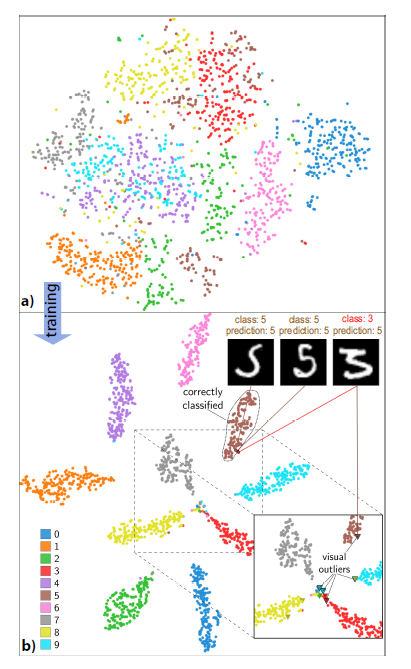
\includegraphics[scale=0.9]{images/embedding_view/HRV_Fig_006_Rauber_B.PNG}
	\caption{Barnes-Hut t-SNE Projection of LeNet5 Before and After Training on Digits MNIST, source: \cite{Rauber2017VisualizingTH}}
	\label{fig:HRV_006_Rauber_B}
\end{figure}

\vspace{0.2cm}

Dense embedding visualisation can also be used to explain model failure, which can provide visual feedback as shown on Figure \ref{fig:HRV_005_Rauber_A}:

\vspace{0.2cm}

\begin{figure}[H]
	\centering
	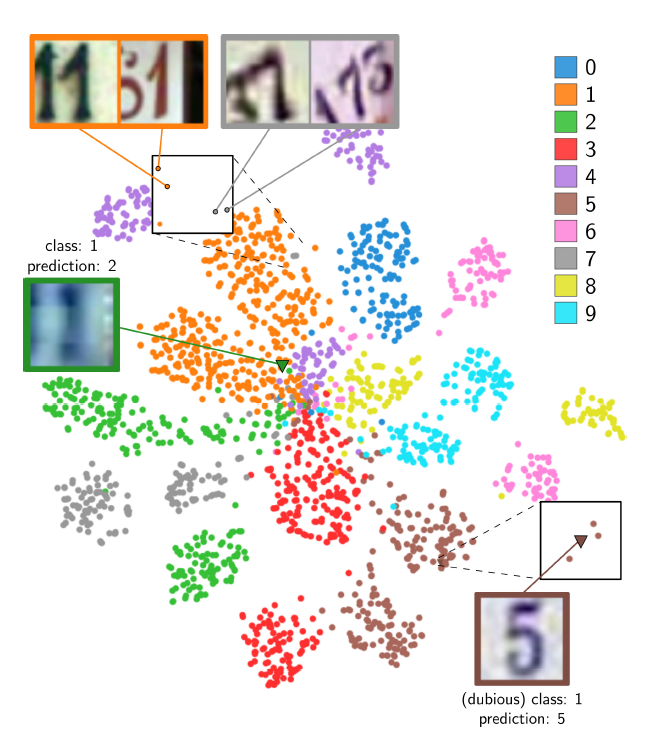
\includegraphics[scale=0.65]{images/embedding_view/HRV_Fig_005_Rauber_A.PNG}
	\caption{Barnes-Hut t-SNE Projection of LeNet5 Before and After Training on SVHN, source: \cite{Rauber2017VisualizingTH}}
	\label{fig:HRV_005_Rauber_A}
\end{figure}

\vspace{0.2cm}

Error analysis on Figure \ref{fig:HRV_005_Rauber_A} can help identify anomalies in our training process and even dataset quality: confusing inputs with different labels cluttering all over the image, similarly looking classes that nevertheless were labelled differently or labelling mistakes (e.g. a clear Digit 5 incorrectly labelled in the validation set as a Digit 1), etc.

The authors do point out a number of caveats to watch out: first, Barnes-Hut t-SNE needed 10 minutes to compute the 2D projections, which while fair for static analysis would be to slow and impractical for a Tensorboard-style framework designed to monitor the training phase of DCNNs. Issues with scalability also pop up when the number of classes are very high (e.g. CIFAR-100, ImageNet). The categorical colour mapping - for assessing how well our model is able to discriminate between different labels - will quickly create visual clutter on our scatter plot, which a continuous colour mapping is unlikely to fix. Finally, while the authors found that embedding visualisation usually led to insightful visual feedback on internal model behaviour, there are no guarantees of success for unsupervised learning methods such as dimensionality reduction and without supplementary metrics from supervised learning (such as accuracy scores for each class, confusion matrices), such visualisations could be misleading.

\subsubsection{Embedding Visualization: Convolutional Layers}
\label{embeddings-convolutional}

Convolutional layer embeddings present a much harder challenge. Dense layer activations can be extracted as matrices, but convolutional layers output multi-channel hidden activations which can be extracted not as matrices but 3D tensors. The most readily-used dimensionality reduction algorithms can only reduce the dimensionality of matrices, not tensors. This explains why until recently the focus of embedding visualisation was exclusively on dense embeddings, as they are easier to plot.

In recent years, there have been attempts to extract the hidden activations of convolutional layers and reduce them to a lower-dimensional space for visualisation. \cite{Pezzotti2018DeepEyesPV} developed DeepEyes' for monitoring the training phase of DCNNs following guidelines from Progressive Visual Analytics. They expanded on initial work over embedding visualisation from \cite{Rauber2017VisualizingTH} for convolutional layers. They randomly sample tens of thousands of patches for each image (known as receptive fields), obtain activations for said patches and project those activations into lower-dimensional space for visualisation with a faster C++ implementation of t-SNE (called Hierarchical t-SNE). As seen on Figure \ref{fig:HRV_007_Pezzotti_A}, we find a similar conclusion to Figure \ref{fig:HRV_006_Rauber_B}: deeper layers tend to be more class specialized, whereas parameter/filter sharing is more prevalent in earlier layers.

\vspace{0.2cm}

\begin{figure}[H]
	\centering
	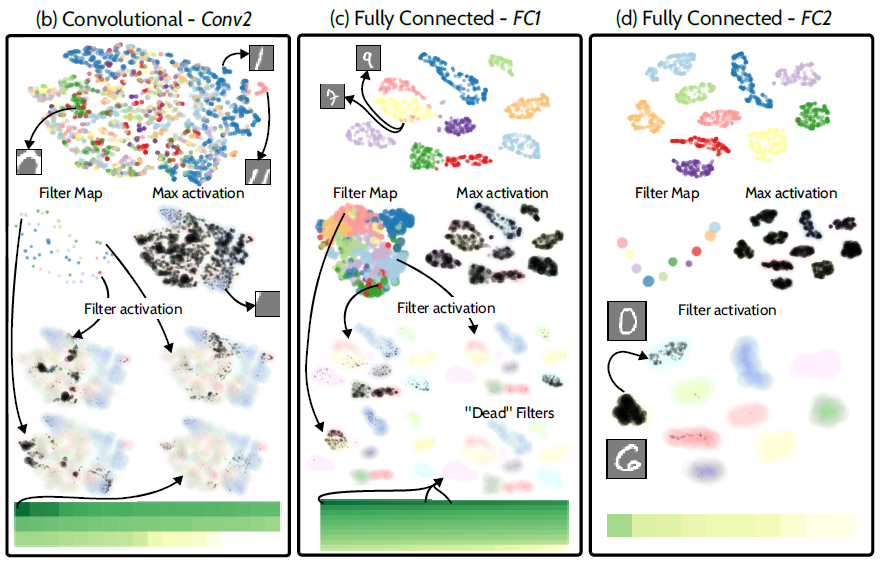
\includegraphics[scale=0.75]{images/embedding_view/HRV_Fig_007_Pezzotti_A.PNG}
	\caption{Hierarchical t-SNE Projection of LeNet5 Layers Before and After Training on MNIST, source: \cite{Pezzotti2018DeepEyesPV}}
	\label{fig:HRV_007_Pezzotti_A}
\end{figure}

\vspace{0.2cm}

This approach for extracting the hidden activations was also utilized by \cite{Carter2019} and \cite{Rathore2019TopoActET} for decoding InceptionV1 on ImageNet. Instead of projecting the receptive fields and plotting them with their respective labels, they run their own feature visualisation techniques on top of those receptive fields. This allows them to explicitly highlight how DCNNs start by detecting edges and textures before moving in later layers to full objects.

Contrasting the aforementioned approaches, \cite{hohman2020summit} - for their visual analytics software Summit - take a different approach: the authors focus on extracting the most useful information out of the convolutional layers channel depth. The authors start by assuming that channels can be more or less interpreted as concepts (e.g. edges, textures, patterns, parts of objects) and that for a given image fed through the convolution layer, the higher the activation values the more representative the concept within the image. As an illustration, for a batch of images passed through a 512-channel convolutional layer, only the maximal activation value is kept for each of the 512 channels. The authors hold that this operation is equivalent to running a Global Maximum Pooling over each layer.

Therefore, images fed through a 512-channel convolutional layer can be described as a 512-dimensional channel vector. This solves the roadblock of representing tensor-shaped convolutional layer activations as high-dimensional vectors. The authors go even further and aggregate each channel vector per class, creating a class-activation matrix, which they then plot down into 2D with UMAP as seen on Figure \ref{fig:HRV_008_Summit}.

\vspace{0.2cm}

\begin{figure}[H]
	\centering
	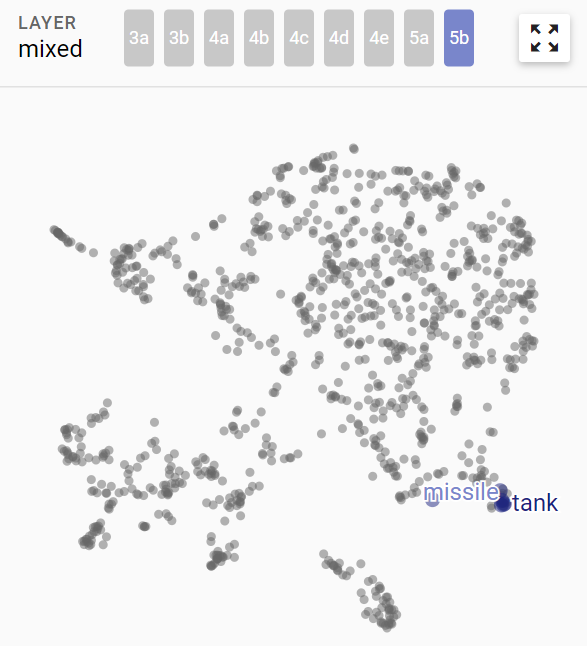
\includegraphics[scale=0.85]{images/embedding_view/HRV_Fig_008_hohman_UMAP.PNG}
	\caption{UMAP Projection of InceptionV1 Mixed5b Layer on ImageNet, source: \cite{hohman2020summit}}
	\label{fig:HRV_008_Summit}
\end{figure}

\vspace{0.2cm}

One major benefit of this approach is that it scales well with an extremely high number of classes as seen on Figure \ref{fig:HRV_008_Summit} with ImageNet dataset's 1000 classes.

\subsubsection{Embedding Visualization: Neuron/Filter Activity}

One limitation of the aforementioned visualizations (at a layer level) is that it ignores examining the relationships between the different filters or neurons and how those groups of parameters interact between each other in order to accomplish their roles (e.g. classification, regression, generative modelling). In light of this, \cite{Rauber2017VisualizingTH} offered a novel approach (at least at the time and for dense layers only) to visualizing how similar neurons co-interact with each other and how dissimilar neurons are in Euclidean sense far apart.

Using the same extraction procedure for visualizing the hidden representations learned by the DCNN, they treat each neuron as a vector described by $n$ layer activations, they start by computing a Pearson correlation matrix $\rho$ between neuron pairs. From this correlation matrix, they compute dissimilarity scores $1 - |\rho_{i,j}|$ for each neuron pair $i$ and $j$. From this dissimilarity matrix of neurons, they project this matrix down to 2D with the help of multidimensional scaling (MDS). MDS is more suited for preserving global relationships between our original data when reduced to a lower-dimensional space. And as the number of dimensions to reduce are small (less than a thousand neurons), the procedure is not bottlenecked by its quadratic complexity of $O(n^2)$. They obtain the following visualization (as seen in Figure \ref{fig:HRV_009_Neuron_Spec}):

\vspace{0.2cm}

\begin{figure}[H]
	\centering
	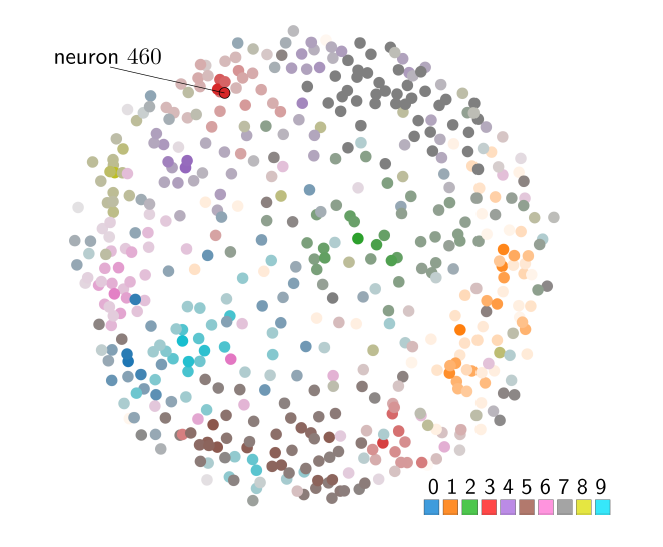
\includegraphics[scale=0.85]{images/embedding_view/HRV_Fig_009_Neuron_Spec.PNG}
	\caption{MDS Projection of Peniultimate Dense Layer Neurons, source: \cite{Rauber2017VisualizingTH}}
	\label{fig:HRV_009_Neuron_Spec}
\end{figure}

\vspace{0.2cm}

The authors highlight one potential application of such visualization: monitor how different regions of a given layer specialize for accomplishing different supervised learning tasks, e.g. on the SVHN dataset, how one set of neurons is mostly active when predicting Digit 3 whereas another region is specialized in detecting Digit 1. They accomplish this by using supervised learning (here extra-randomized trees) to output a discriminative score for each neuron, measuring the associative strength of a neuron with a given label.

The aforementioned visualization from \cite{Rauber2017VisualizingTH} only works on dense layers. \cite{Pezzotti2018DeepEyesPV} extended the aforesaid authors' work for convolutional layers.


\vspace{0.2cm}

\begin{figure}[H]
	\centering
	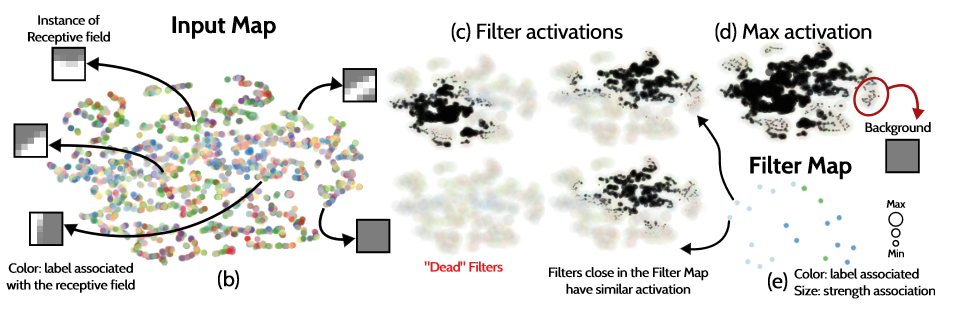
\includegraphics[scale=0.85]{images/embedding_view/HRV_Fig_010_Dead_Zones.PNG}
	\caption{Hierarchical t-SNE Projection of Convolutional Layer Activations (Input Map) and Filters (Filter Map), source: \cite{Pezzotti2018DeepEyesPV}}
	\label{fig:HRV_010_Dead_Zones}
\end{figure}


\vspace{0.2cm}

Filters structure convolutional layers, which differ significantly from dense layer neurons in that they are 3-dimensional tensors (for width, height and number of channels). Thus, \cite{Pezzotti2018DeepEyesPV} uses an alternative distance metric (different from Pearson correlation) for computing the filter similarity: a custom Jaccard similarity distance $\phi_{i,j}$ between two convolutional layer filters $i$ and $j$. Once a similarity matrix $\phi$ is computed, just as in the case of dense layers, the similarity matrix is brought down to a 2-dimensional plane (here with the help of t-SNE) and easily visualized on a 2D scatterplot. Finally, each filter is colored differently, depending on how often a filter responds to a particular label (hinting at specialization). For each filter, an internal metric (described in greater detail in the authors' paper) keeps tabs of how strongly it reacts to all labels.


An example from \cite{Pezzotti2018DeepEyesPV} is provided on Figure \ref{fig:HRV_010_Dead_Zones} through the authors' Filter Map. Interacting with a specific filter on the Filter Map highlights the observations that reacted the most strongly with the selected unit. This functionality allows model designers to quickly identify redundant filters that almost never fire off (although manually pruning superfluous units is no guarantee of improved performance).


\subsection{Interactive Viewer with Plotly Dash}

\subsubsection{Deep Embedding Viewer (i): Motivation}

To synthesize work across different research papers, an interactive prototype was developped as a synthesis and a Proof-Of-Concept of how Embedding Visualization can be put to use for different use-cases: e.g. model comparison, training phase monitoring, adversarial training, etc. An illustration of our viewer's goal is provided below (Figure \ref{fig:HRV_011_DEV_Schema}):


\vspace{0.2cm}

\begin{figure}[H]
	\centering
	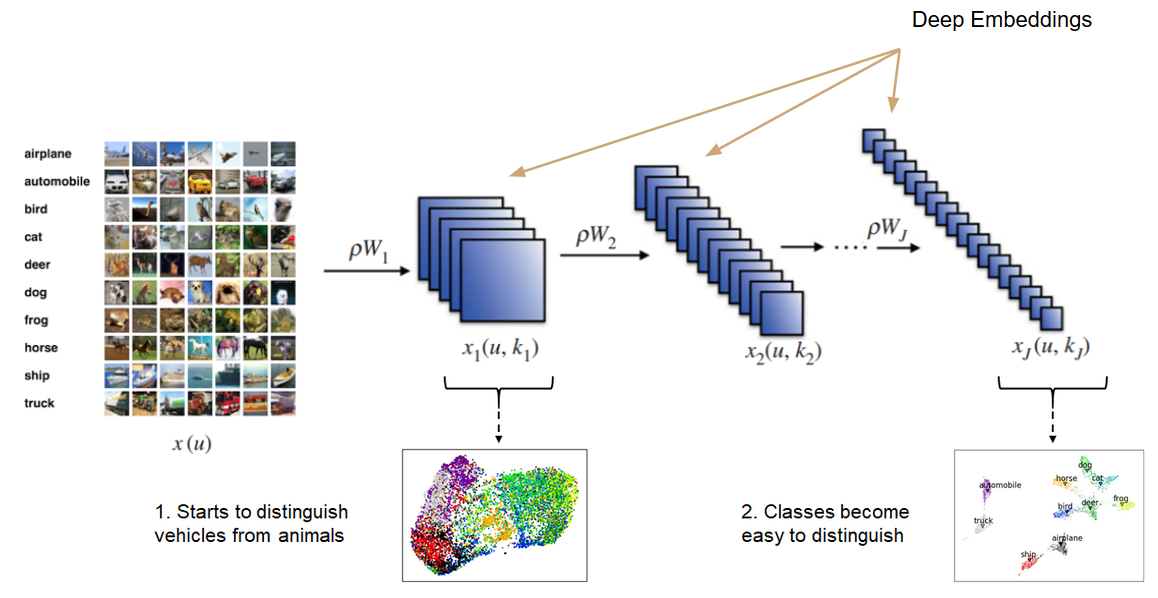
\includegraphics[scale=0.65]{images/embedding_view/HRV_Fig_011_Schema.PNG}
	\caption{Deep Embedding Viewer (with Plotly Dash): Illustrative Schema}
	\label{fig:HRV_011_DEV_Schema}
\end{figure}

\vspace{0.2cm}


Since production deployment in a real-life environment is not the purpose of this research venture, Plotly Dash was chosen as our interactive visualization library. Dash allows for quickly prototyping dashboards without the verbose development infrastructure of more sophisticated visualization frameworks (such as D3.js). 

Our interactive viewer - named \textbf{Deep Embedding Viewer} - takes a Keras model and an available dataset (limited to CIFAR-10 for this research project). Extending our viewer to Tensorflow 2.0 and PyTorch models or alternative datasets is out-of-scope. Keras models are to be dropped into a specific folder from which dropdown selection allows the user to easily select and even later swap between different models (as seen on Figure \ref{fig:HRV_011_DEV_Intro}).


\vspace{0.2cm}

\begin{figure}[H]
	\centering
	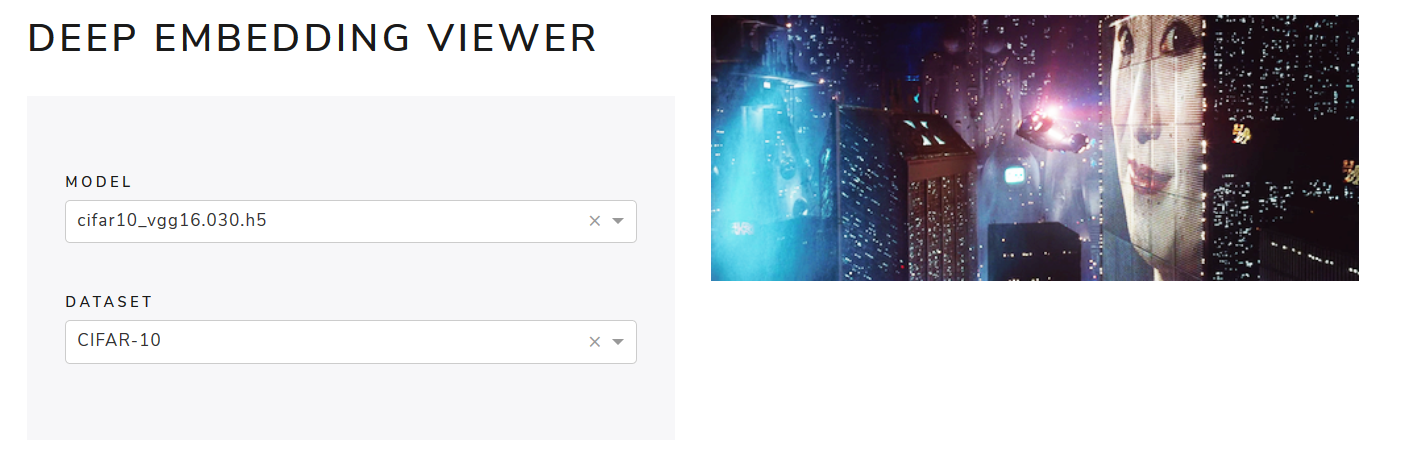
\includegraphics[scale=0.55]{images/embedding_view/HRV_Fig_011_DEV_Intro.PNG}
	\caption{Deep Embedding Viewer (with Plotly Dash): Keras Model and Dataset Selection}
	\label{fig:HRV_011_DEV_Intro}
\end{figure}

\vspace{0.2cm}

Once a model and dataset were chosen, our viewer loads a total of five panels:

\begin{enumerate}
	\item Learned Representations View
	\item Image Viewer
	\item Neuron Activity Map
	\item Model Performance Analysis
	\item Adversarial Robustness Simulation
\end{enumerate}

The viewer fully utilizes Plotly Dash's callback system for creating dependencies between the different panels, allowing for a user to swap between different models of his choosing (as seen Figure \ref{fig:HRV_Fig_019_DEV_Callback_Structure}).

\newpage


\begin{figure}[H]
	\centering
	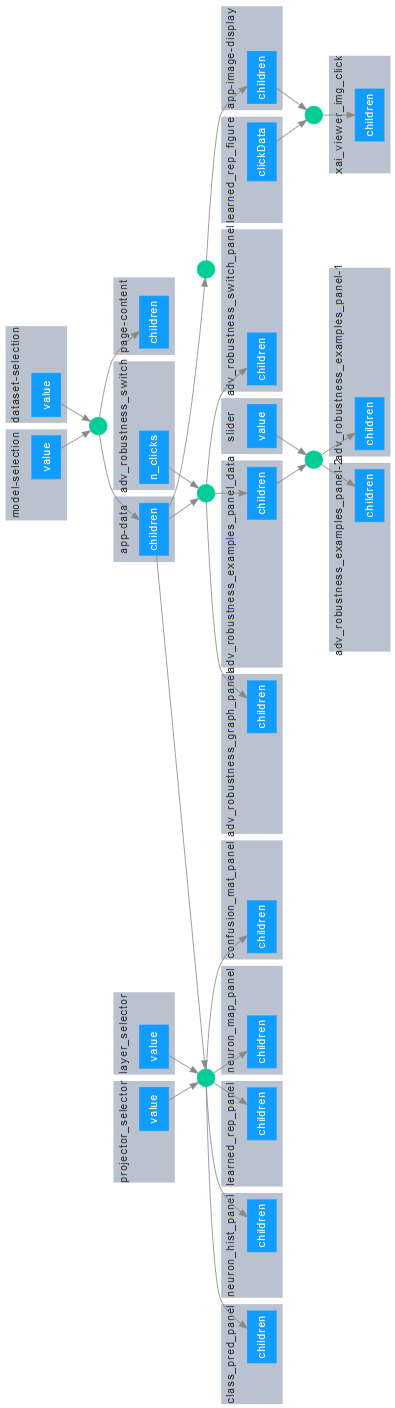
\includegraphics[scale=0.9]{images/embedding_view/HRV_Fig_019_DEV_Callback_Structure.PNG}
	\vspace{0.2cm}
	\caption{Deep Embedding Viewer (with Plotly Dash): Callback Structure}
	\label{fig:HRV_Fig_019_DEV_Callback_Structure}
\end{figure}

\newpage


\subsubsection{Deep Embedding Viewer (ii): Learned Representations View / Image Viewer}

The showcase of our viewer is the \textbf{Learned Representations View} for visualizing DCNN embeddings on a 2-dimensional scatterplot. It is heavily inspired from much of the research literature presented in the earlier subsections. It is capable of handling both dense and convolutional layers. Specifically, for dense layers, it follows closely work from \cite{Rauber2017VisualizingTH} with the sole exception that UMAP - a more computationally-efficient nonlinear dimensionality reduction algorithm - replaces t-SNE. In the case of convolutional layers, we opted for a streamlined version of the methodology implemented on \cite{hohman2020summit}, instead of the receptive field approach used instead by \cite{Pezzotti2018DeepEyesPV} and \cite{Carter2019}. The former was simply easier to implement than the latter.

Since we are interested in how our DCNN is reacting to data and understand the nature of its decision-making process, we will use a randomly sampled version of CIFAR-10 dataset's training data (forming a validation set) that was not used during the entirety of the training process.

For the scatterplot itself, Plotly Dash provides user interactivity and one such application is image display through the \textbf{Image Viewer}. In addition to colouring each embedded image with its respective label, to help reminder the viewer that the dots on the scatterplot are supposed to represent images, simply clicking on any unit will display its corresponding image. Selecting an embedding image with a correct prediction ensues the following display (Figure \ref{fig:HRV_016_DEV_Image_Viewer_1}):

\vspace{0.2cm}

\begin{figure}[H]
	\centering
	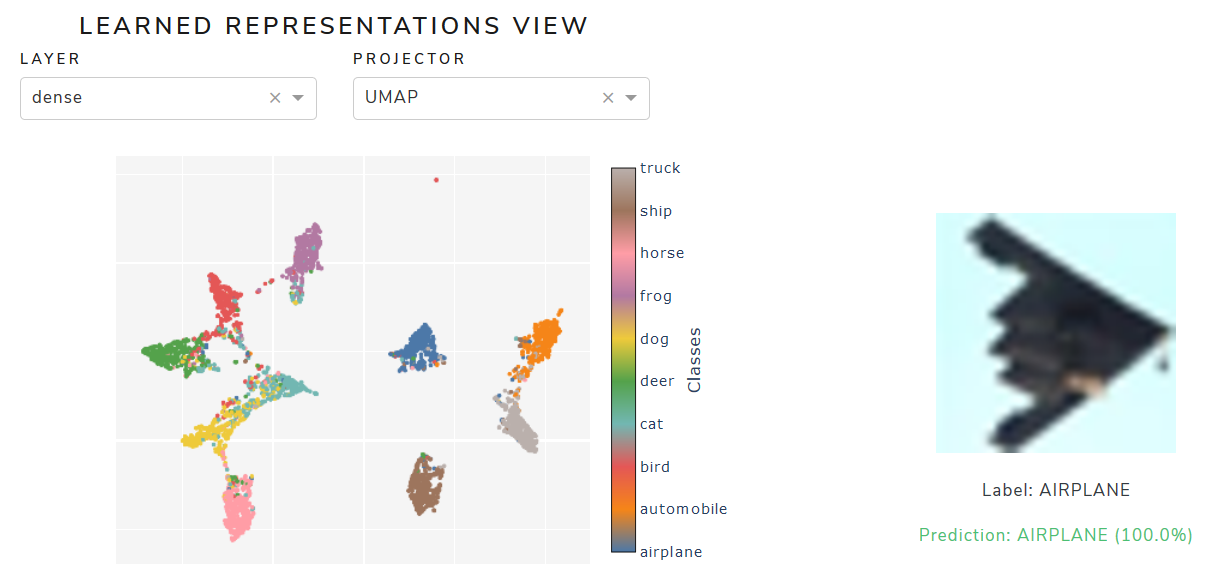
\includegraphics[scale=0.65]{images/embedding_view/HRV_Fig_016_DEV_Layer_Embedding.PNG}
	\caption{Deep Embedding Viewer (with Plotly Dash): Learned Representations View with an Accurate Prediction}
	\label{fig:HRV_016_DEV_Image_Viewer_1}
\end{figure}

\vspace{0.2cm}

Conversely, a selected embedding image with an incorrect prediction will result in the following (cf. Figure \ref{fig:HRV_016_DEV_Image_Viewer_2}):

\vspace{0.2cm}

\begin{figure}[H]
	\centering
	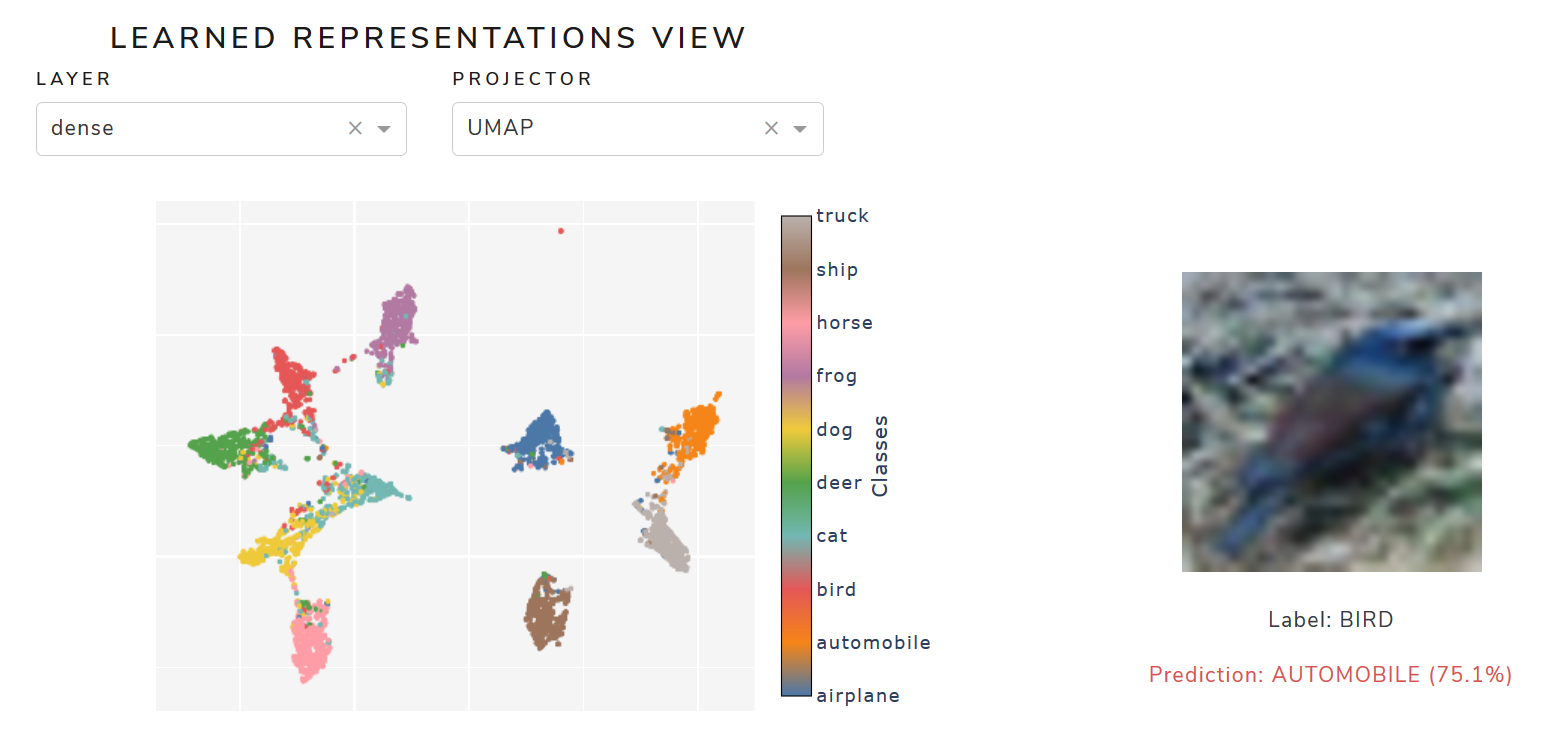
\includegraphics[scale=0.55]{images/embedding_view/HRV_Fig_016_DEV_Layer_Embedding_1.PNG}
	\caption{Deep Embedding Viewer (with Plotly Dash): Learned Representations View with an Incorrect Prediction}
	\label{fig:HRV_016_DEV_Image_Viewer_2}
\end{figure}

\vspace{0.2cm}

Integral to the viewer is the ability to switch between different layers, confirming that moving into increasingly deeper layers leads to increasing specialization within our DCNN:



\vspace{0.4cm}

\begin{figure}[H]
	\begin{minipage}{0.48\textwidth}
		\centering
		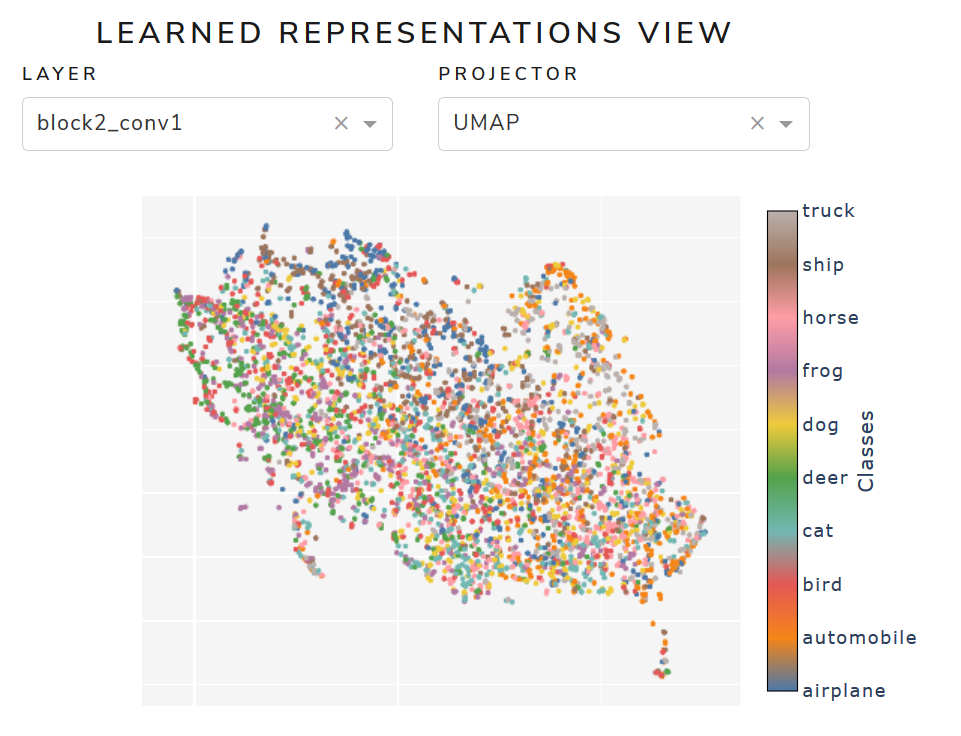
\includegraphics[width=1\linewidth]{images/embedding_view/HRV_Fig_015_DEV_Embedding_4.PNG}
		\caption{UMAP 2D Visualization of VGG-16 block2\_conv1 Convolutional Layer}\label{Fig:HRV_Fig_015_DEV_Embedding_4}
	\end{minipage}\hfill
	\begin{minipage}{0.48\textwidth}
		\centering
		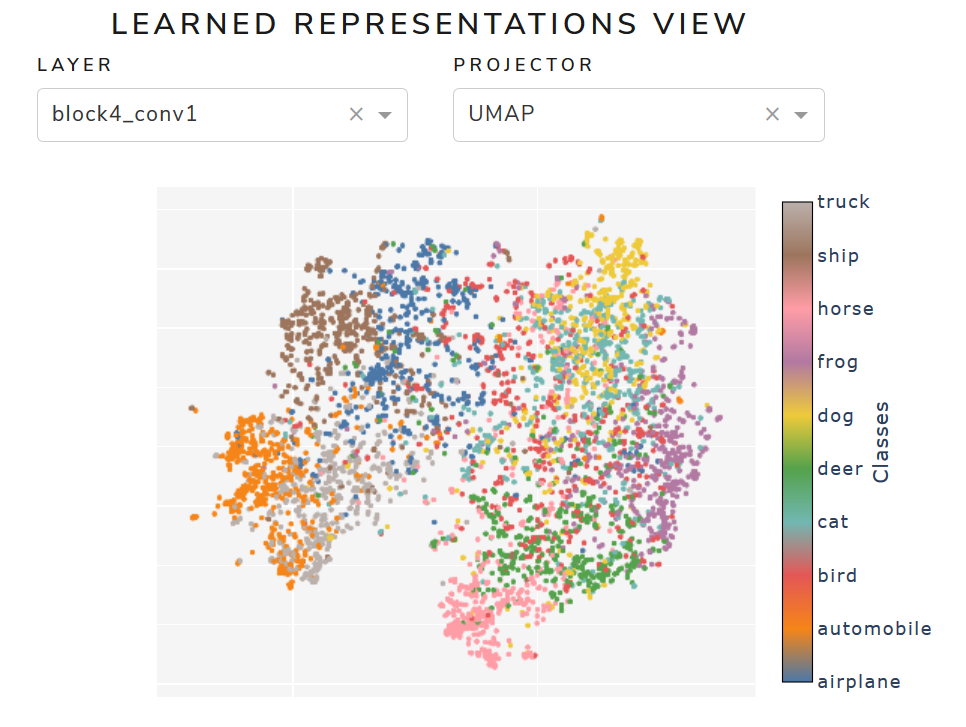
\includegraphics[width=1\linewidth]{images/embedding_view/HRV_Fig_014_DEV_Embedding_3.PNG}
		\caption{UMAP 2D Visualization of VGG-16 block4\_conv1 Convolutional Layer}\label{Fig:HRV_Fig_014_DEV_Embedding_3}
	\end{minipage}
\end{figure}

\vspace{0.2cm}


And different dimensionality reduction methods, e.g. between PCA and UMAP. Although UMAP is the default and preferred approach for our viewer, a more computationally friendly implementation of t-SNE can be used as an alternative:

\vspace{0.2cm}

\begin{figure}[H]
	\begin{minipage}{0.48\textwidth}
		\centering
		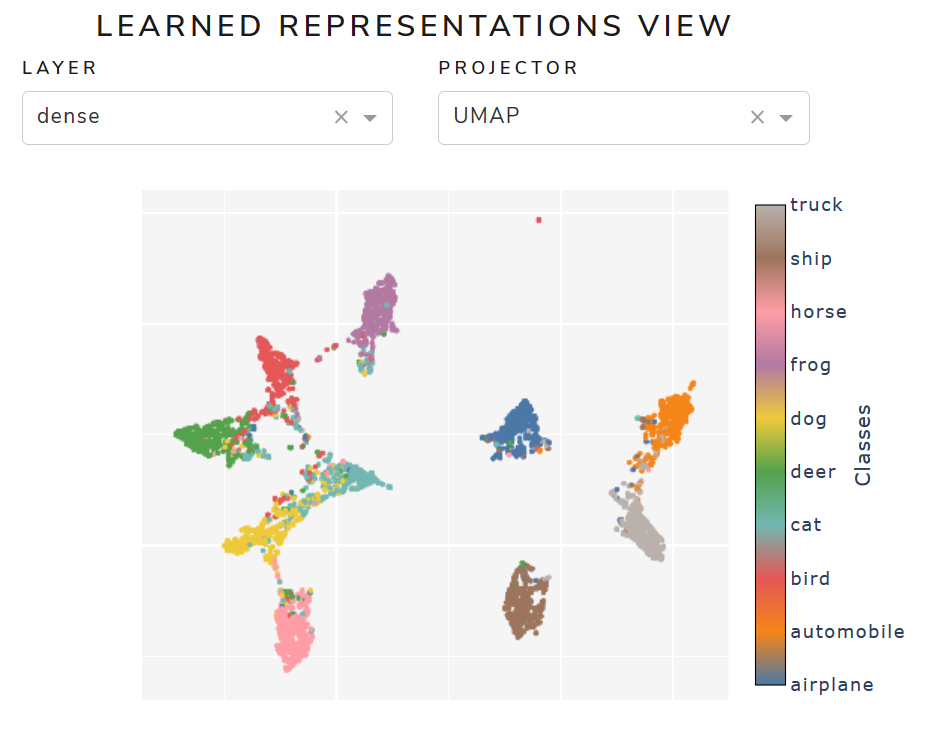
\includegraphics[width=1\linewidth]{images/embedding_view/HRV_Fig_012_DEV_Embedding_1.PNG}
		\caption{UMAP 2D Visualization of VGG-16 Penultimate Dense Layer}\label{Fig:HRV_Fig_012_DEV_Embedding_1}
	\end{minipage}\hfill
	\begin{minipage}{0.48\textwidth}
		\centering
		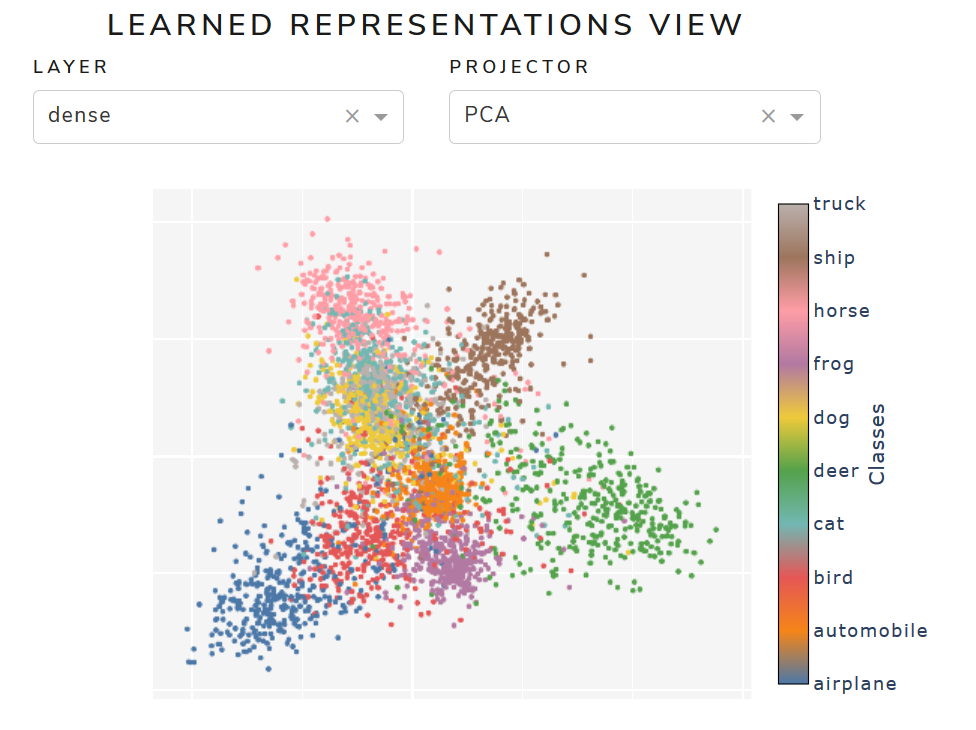
\includegraphics[width=1\linewidth]{images/embedding_view/HRV_Fig_013_DEV_Embedding_2.PNG}
		\caption{PCA 2D Visualization of VGG-16 Penultimate Dense Layer }\label{Fig:HRV_Fig_013_DEV_Embedding_2}
	\end{minipage}
\end{figure}

\vspace{0.2cm}
 
\subsubsection{Deep Embedding Viewer (iii): Neuron Activity Map}

Our application supplements the Learned Representations View with the \textbf{Neuron Activity Map} for visualizing behavioural similarities between neurons and filters (for dense and convolutional layers respectively). Our implementation is a synthesis of three different research papers: (1) the initial blueprint provided by \cite{Rauber2017VisualizingTH}, (2) the use of an alternative distance metric (differing from Pearson correlation) in \cite{Pezzotti2018DeepEyesPV} and (3) the methodology used by \cite{hohman2020summit} for extracting embeddings out of convolutional layers.


For a more detailed description of our implementation, we will start with dense layers. To simplify our analysis of neuron/filter relationships, we start by taking only the absolute values of layer activations. Next, a cosine distance matrix is computed on top of those layer activations. Thus, we obtain the degree of similarity between different neurons (e.g. a layer embedding composed of 10,000 observations described by 200 neurons yields a cosine distance matrix of dimensions $200 \times 200$). This cosine distance matrix is then reduced to 2-dimensional space with the UMAP algorithm (with a specific set of hyperparameters chosen) and plotted on a 2D scatterplot. This entire process is the same for convolutional layers, with the added difference that the methodology from \cite{hohman2020summit} is applied before computing the cosine distance matrix to obtain the necessary convolutional embeddings.


As for our choice to use the cosine distance matrix, it is due to its ability to handle sparse embedding vectors (unlike methods such as the Pearson correlation) and how the output is bounded between 0 and 1. It is also partially due to the fact that the cosine measure is heavily used in the field of NLP for computing the distance between word embeddings.

This panel is directly intertwined with the Learned Representations View, as switching between different layers yields a different view of layer activations and neuron/filter similarities:


\vspace{0.2cm}

\begin{figure}[H]
	\begin{minipage}{0.48\textwidth}
		\centering
		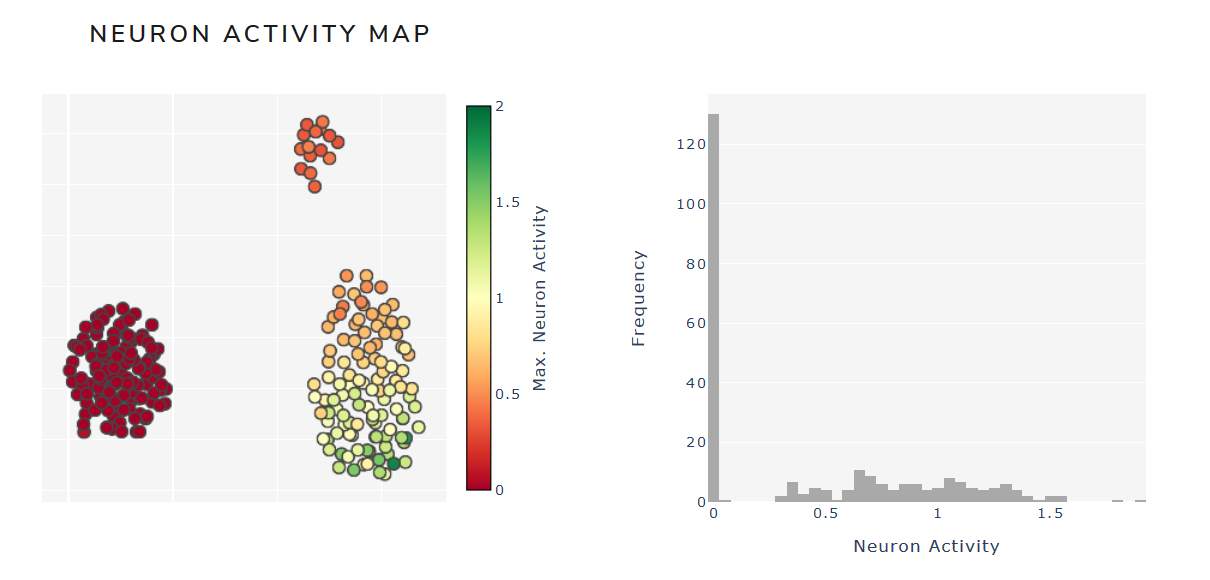
\includegraphics[width=1\linewidth]{images/embedding_view/HRV_Fig_017_DEV_Neuron_Embedding.PNG}
		\caption{UMAP 2D Visualization of VGG-16 Penultimate Dense Layer Neurons}\label{Fig:HRV_Fig_017_DEV_Neuron_Embedding}
	\end{minipage}\hfill
	\begin{minipage}{0.48\textwidth}
		\centering
		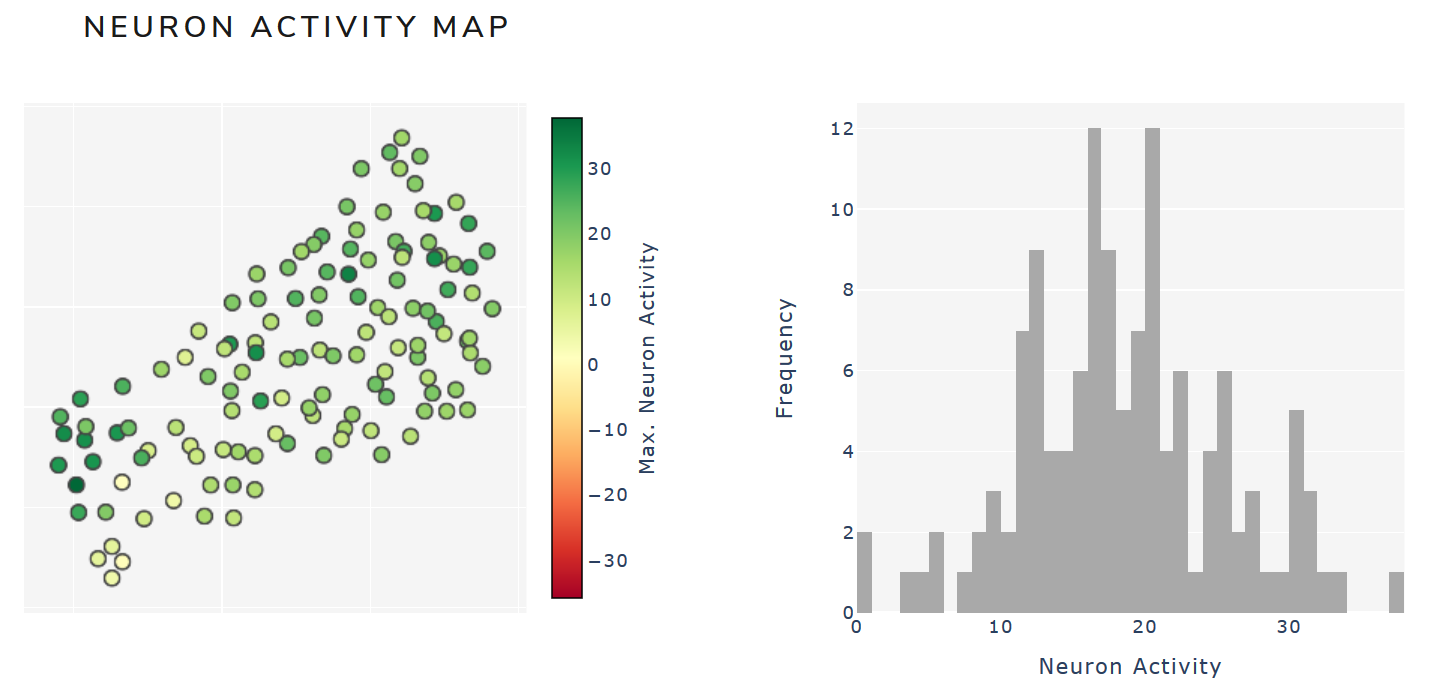
\includegraphics[width=1\linewidth]{images/embedding_view/HRV_Fig_018_DEV_Neuron_Embedding_2.PNG}
		\caption{UMAP 2D Visualization of VGG-16 block4\_conv1 Filters}\label{Fig:HRV_Fig_018_DEV_Neuron_Embedding_2}
	\end{minipage}
\end{figure}


\vspace{0.2cm}

Unlike the Learned Representations View, UMAP is the only provided option for visualizing neuron/filter similarities.

\subsubsection{Deep Embedding Viewer (iv): Model Performance Analysis}

Our initial viewer lacked basic information on the DCNN's actual performance. Thus, we supplement the previous visualizations with simple but effective performance metrics - \textbf{Normalized Confusion Matrix} and \textbf{Class Prediction Accuracy} - that will help the user understand the results obtained in the Learned Representations View and Neuron Activity Map. Visual clutter in the Learned Representations View when visualizing the penultimate layers before softmax classification is likely to be indicative of label confusion (e.g. dogs confused as cats in the case of CIFAR-10), which can be confirmed with the confusion matrix.




\vspace{0.2cm}

\begin{figure}[H]
	\centering
	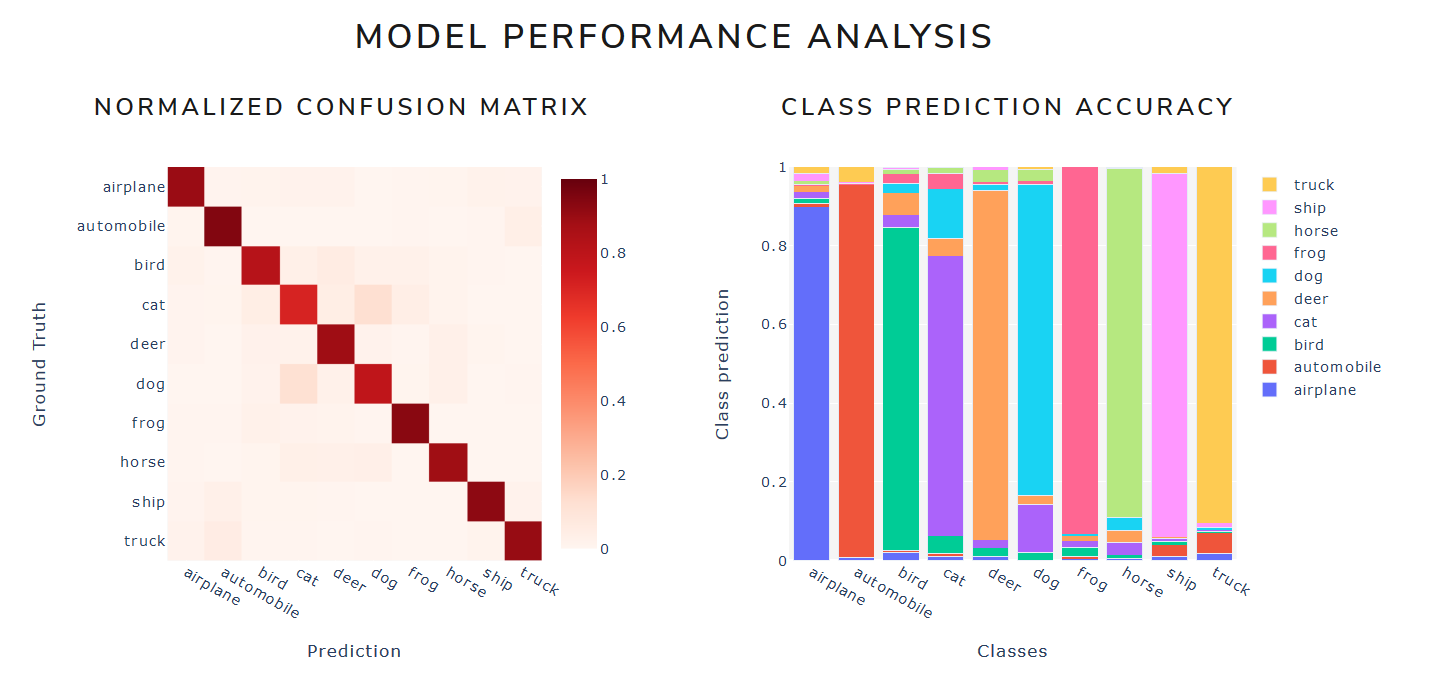
\includegraphics[scale=0.55]{images/embedding_view/HRV_Fig_011_DEV_Metrics.PNG}
	\caption{Deep Embedding Viewer (with Plotly Dash): Model Performance Analysis}
	\label{fig:HRV_Fig_011_DEV_Metrics}
\end{figure}

\vspace{0.2cm}

Complementing embedding visualization with performance metrics is also further recommended by 
\cite{Rauber2017VisualizingTH} for improving the reliability and the relevance of embedding visualization.


\subsubsection{Deep Embedding Viewer (v): Adversarial Robustness Simulation}

Although elaborated in greater detail in a previous section, \textbf{Adversarial Robustness Simulation} is provided as an additional panel (at the end of the viewer) for stress testing convolutional neural networks against FGSM-generated adversarial attacks.

 % Embeddings
\newpage

\section{Deep Neural Network Monitor}
\label{sec6}

\subsection{Objectives and intuitions}

One of objectives of this project is to visualise, or ``monitor'' the CNN behaviour during the training phase. Thanks to the previous mentionned methods, users will have insights about the training phase and judge if the CNN has a strong or over-sized architecture and right parameters. Also, one might get visual indications on whether the training is running smoothly and the parameters converge to their correct values, or on the contrary whether training is ill-behaved and should re-initiated.
 
As we show in section \ref{sec2}, weights and gradients constitute key elements of deep neural networks. However, it is too complex to assess the quality of a CNN from brute values of weights and gradients at each epoch. It is therefore necessary to create custom metrics around gradients and weights to detect specific patterns like black areas, or highest and lowest activation areas of our network.

The custom metrics are the following :
\begin{itemize}
    \item loss and accuracy values for training and validation samples
    \item difference of weights between 2 consecutive epochs
    \item absolute value of gradients for one epoch
	\item activation map for each filter of the selected layer
	\item correlation between filters of the selected layer
\end{itemize}

The application developed in this section is largely based on the paper by \cite{Chen2018}. The latter proposes a number of visualisation techniques, in particular for the representation of weights, gradients, and activations along with their correlations. It is also the one paper demonstrated by the Ministry of Defense during their initial presentation, so the proposed visualisations were also part of the agenda for the project.

\subsection{Overview}


\subsubsection{Overall design}


Our application frontend comes as a dashboard (or graphical interface) composed of four quadrants:

\begin{enumerate}
	\item design of the network architecture
	\item loss and accuracy curves
	\item weights and gradiants visualization
	\item activation and correlation maps
\end{enumerate} 

The interface is fairly compact because we consider the tool as a POC \emph{(proof of conception)}. Developing a more user-friendly interface may constitute an improvement axis for further developments. For now, this framework proves suitable and convenient. 

\begin{figure}[H]
	\centering
	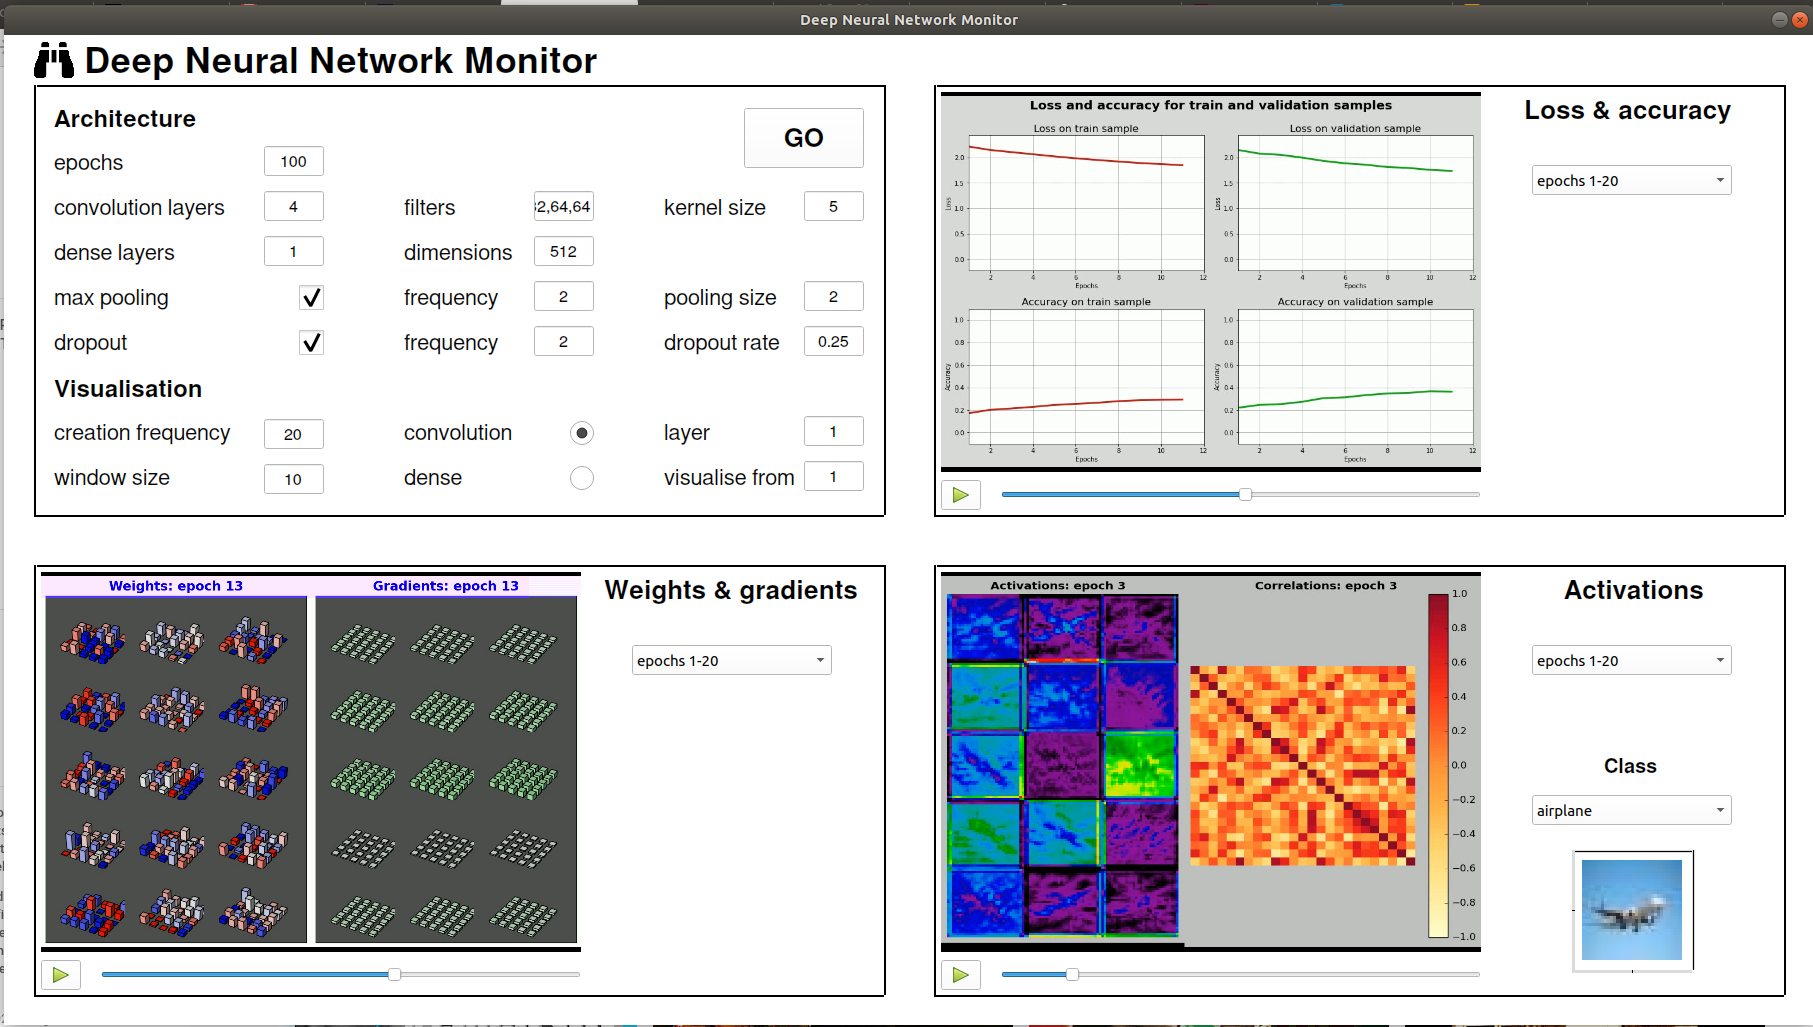
\includegraphics[scale=0.32]{images/weights-grads-viewer/frontend.png}
	\caption{Our application frontend}
\end{figure}

The backend consists in a set of modules with custom functions that need to be imported prior to starting the application. The python code then calls a Keras API which runs the designed CNN on the CIFAR 10 dataset. The information required for our visualizations is extracted by the way of callback functions and checkpoint processings, both included in tensorflow. Stream processing then provides visualisation in real time.

\begin{figure}[H]
    \centering
    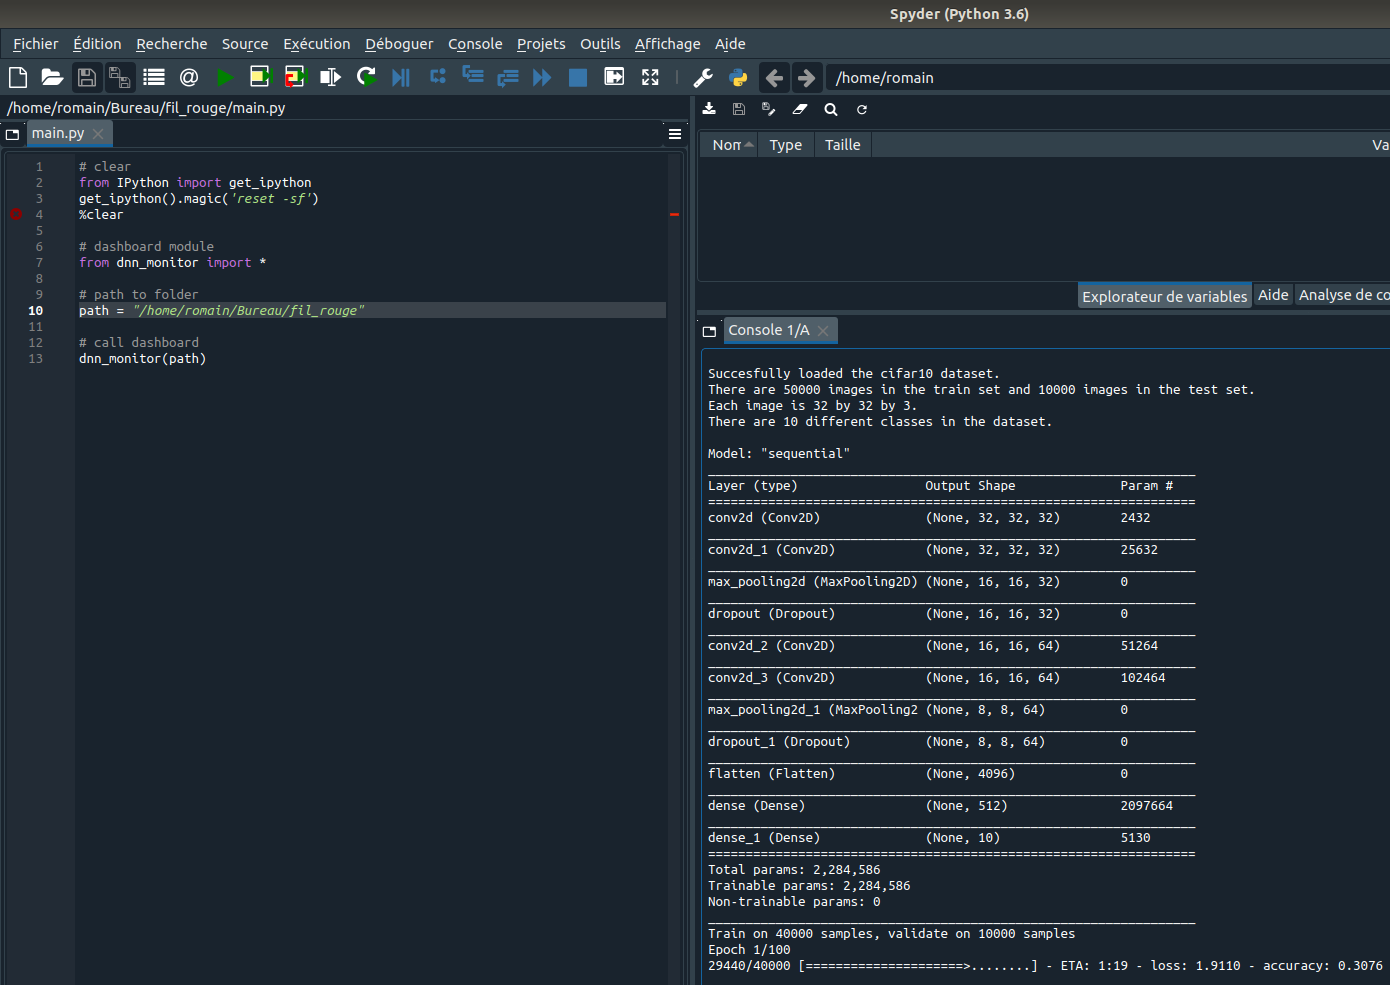
\includegraphics[scale=0.41]{images/weights-grads-viewer/backend.png}
    \caption{Backend: custom code and Keras API}
\end{figure}

\subsubsection{Model architecture}

The first step of our visualization device consists in determining the model architecture. The first quadrant of the dashboard is dedicated to this task and permits to set a number of options, offering some freedom in the design of the model. Among the options to be set are:

\begin{itemize}
    \item the number of convolution layers and the number of filters for each layer, along with the convolution kernel size
    \item the number of dense layers and their respective dimensions
    \item the use of max pooling and dropout with their frequencies and dimensions
\end{itemize} 

In terms of visualization, the lower part of the quadrant proposes to select:

\begin{itemize}
	\item the layer and neurons to be visualized
	\item the frequency at which the visualization must be updated in the dashboard
	\item the window size for the loss/accuracy plots of the second quadrant
\end{itemize} 

\begin{figure}[H]
    \centering
    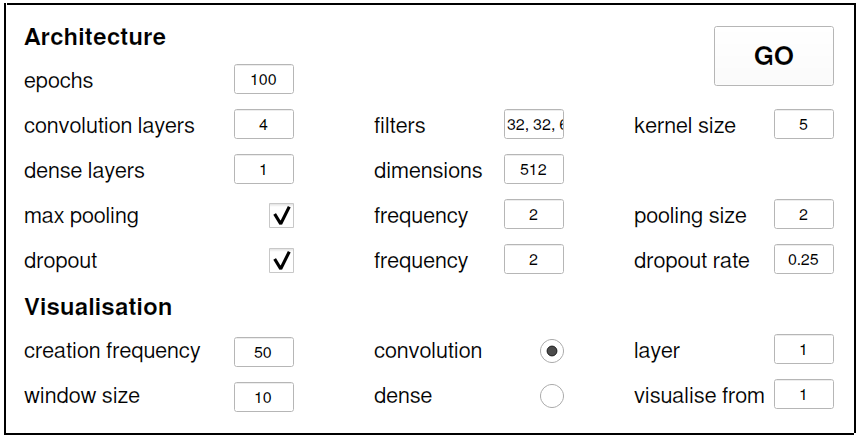
\includegraphics[scale=0.5]{images/weights-grads-viewer/Quadrant_architecture.png}
    \caption{We can customize our DNN thanks to the architecture quadrant}
\end{figure}


\subsection{Custom metrics}

\subsubsection{Accuracy and loss curves}

Accuracy and loss represent two basics metrics, but they are absolutly essential to follow the right or bad behavior of our network during training phase. Moreover, as is customary, we have split our reference dataset into two parts: train and validation. This provides a straightforward way to detect overfitting.   

\begin{figure}[H]
    \centering
    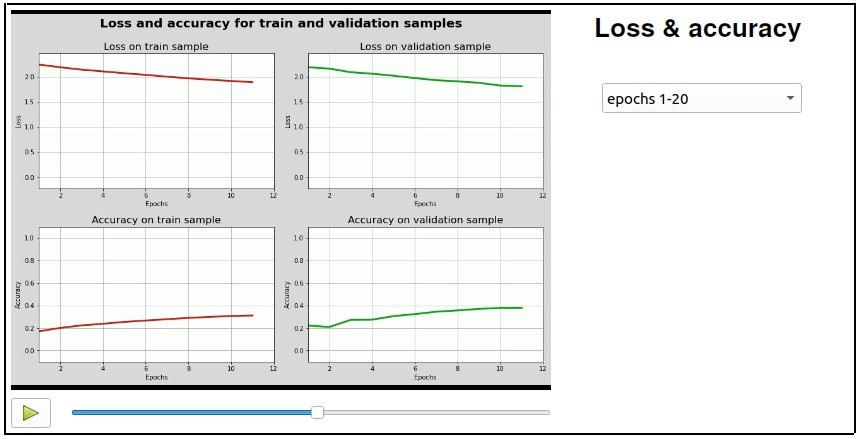
\includegraphics[scale=0.6]{images/weights-grads-viewer/Quadrant_loss.png}
    \caption{Evolution of loss and accuracy across epochs, for train and validation samples}
\end{figure}


\subsubsection{Gradients and Weights}

In this quadrant, we implemented a specific visualisation of weights and gradients evolution. In the panel, the left part is dedicated to weights while the right part represents the gradients. 

Regarding the weights:

\begin{itemize}
	\item red weights are positive, blue weights are negative
	\item the heights of the bars represent the weight value (in absolute value, after normalisation).
	\item the growth rate with respect to the previous period is represented by  color intensity. Pale weights evolve little, while intense color weights keep being updated.
	\item the weights are arganised by flattening filters over a row.
	\item a weight that never evolves and remains flat can be a ``dead'' weight that does not train properly
	\item a weight which keeps updating forever may indicate a difficulty of the model to converge to minimum of the loss function
\end{itemize} 

As for the gradients:

\begin{itemize}
	\item they are always displayed in green
	\item the size of the bars represents the (absolute and standardised) value of the gradient
	\item the color intensity is another proxy for the size, to help further distinguish strong from weak gradients
	\item a high gradient involves a weight still being updated (from back-propagation), a small gradient implies little update
\end{itemize}

\begin{figure}[H]
    \centering
    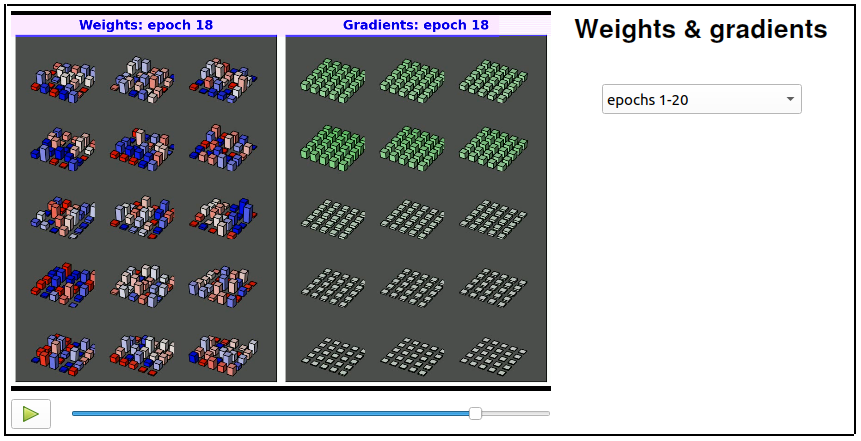
\includegraphics[scale=0.6]{images/weights-grads-viewer/Quadrant_weight.png}
    \caption{Evolution of gradients and loss for convolutional filters}
\end{figure}

\subsubsection{Activations and correlations}

The final metrics developped in the application consists in a display of the activation maps produced by the selected layer (on the left), and their correlations (on the right).

For activations:

\begin{itemize}
	\item each small square in the image represents the activation obtained from one filter of the layer
	\item the activation displayed is actually an average activation obtained over a batch of the class considered (small-sized: 10 images per batch)
	\item it is remarkable that even though the activations are obtained from a batch, they often produce recognizable images (like a ship on the example displayed below)
	\item an activation which remains dark is indicative of a ``dead'' filter which does not train properly
	\item two activations that look very similar may be a flag for redundant filters
\end{itemize}

Regarding correlations:

\begin{itemize}
	\item correlations are represented as a heatmap, where each square represents the correlation between two filters of the layer.
	\item the color code is a range from light yellow (strong negative correlation) to dark red (strong positive correlation)
	\item off-diagonal entries that are dark red imply a correlation close to 1 and thus suggest redundant filters
	\item off-diagonal entries that are light yellow imply a correlation close to -1 and may imply filters having similar but opposite effects
\end{itemize}


\begin{figure}[H]
	\centering
	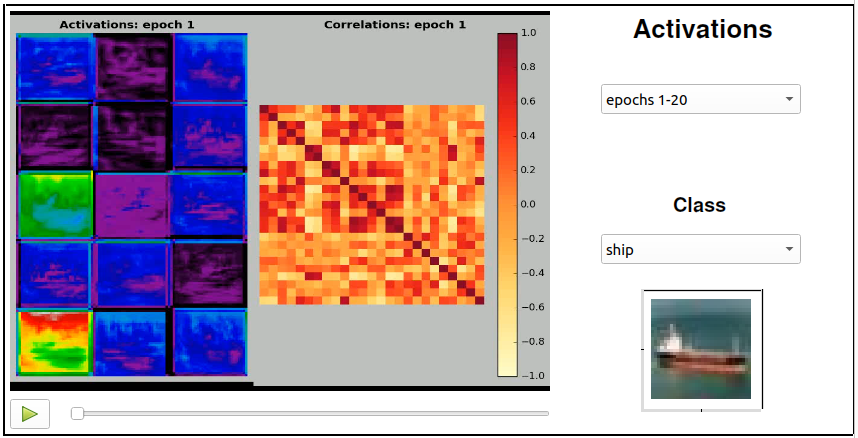
\includegraphics[scale=0.6]{images/weights-grads-viewer/Quadrant_activation.png}
	\caption{Evolution of activations and correlations for convolutional filters}
\end{figure}


\subsubsection{Conclusions on the DNN Monitor}

The DNN monitor provides a compact, intuitive and immediate view on a neural network across the different epochs of the training. One of its major assets is that it makes visualisation possible while training continues running in the background.

Individual views provided by the DNN Monitor can be useful, but it is really the conjugation of losses, accuracies, weights, gradients, activations, correlations and their evolution across training epochs which permits to obtain an overall assessment of the quality of the traning.









 % Weights and Gradients
\newpage

\section{Deep Neural Network Viewer}
\label{sec-dnnviewer}

Deep Neural Network Viewer (DNN Viewer) is a graphical user interface (GUI) showing at the same time the structure, the parameters (weights, intercepts...) and the performance on test data. It is based on the following observations:
 \begin{itemize}
     \item As underlined in \ref{sec5}, activations, saliency (see \ref{sec2}) and occlusion maps, and adverse examples (see \ref{sec3}) provide a very focused views on a single unit or a single layer within a network. However, such views of the DNN do not show overall structure and performance of the network.
     \item The atlases of \ref{sec4} and the embeddings of \ref{sec5} provide an answer to one missing dimension: a global assessment of the unit, layer or network over a full test dataset. But they are missing a representation of the architecture of the network and are not able to show dependencies between neuron units. 
     \item Many available online tools to visualize a DNN are describing the network graph structure, they are not displaying the weights nor assessing the current performance. Among these tools, we may cite Netron (\cite{roeder2020}) which is very comprehensive when it comes to describe the network architecture and supports many formats (Tensorflow, Torch, Caffe...). 
     \item Tensorflow Playground (\cite{tf-playground2020}) goes in the direction of overall network interpretability but is very limited and constrained on network topologies.
     \item Tensorboard provides a mix of structure presentation (Graphs tab), current training parameters (Distributions and Histograms tabs) and performance (Images tab) but there is no link between each of these.
 \end{itemize}

With the DNN Viewer, our aim is to facilitate inspection of the network, to understand the relationship between units, layers and performance on test data. Our intuition is that each neuron power lies within the inter-relationship with other units, and must be evaluated with data samples related to the task accomplished by the model. Also, interpretation cannot be based exclusively on either singular values (i.e. some unit weight or activation), or aggregated values (i.e. layer weights histogram, class average activation), that is why a GUI providing access and switch between these views is very useful to the person in charge of the interpretation.

\ul{As a first step}, 
the DNN Viewer capabilities are limited to \ul{Keras Sequential models} and its main target is images. It can be used with other type of datasets but the displays are then less interesting. 
It will be later extended to other architectures. \ul{DNN Viewer is to be used as a DNN pedagogical tool, and will not scale on medium to large models} since the computation required is too long for an interactive GUI; however we could modify the implementation to only show a section of the DNN and thus limit the required computing load.

The DNN Viewer has been successfully tested with various image classifiers and generative adversarial networks (GAN).

Remaining of this chapter is organized as follows. First a quick overview of the functionality, then some details on the architecture and implementation, and eventually some typical use case and findings.


\subsection{Overview}
\label{dnn-viewer-overview}


DNN Viewer is a Web browser application that is loading from files a sequence of models in over training epochs, and displaying several views. The screen is divided in three main sections. The top section contains the forward and backward buttons to select the epoch to be displayed. Middle section is the main view on the network with a side panel showing network properties. Bottom section has four quadrants showing the input test data, layer properties, unit properties and activation maps.

\begin{figure}[H]
    \centering
    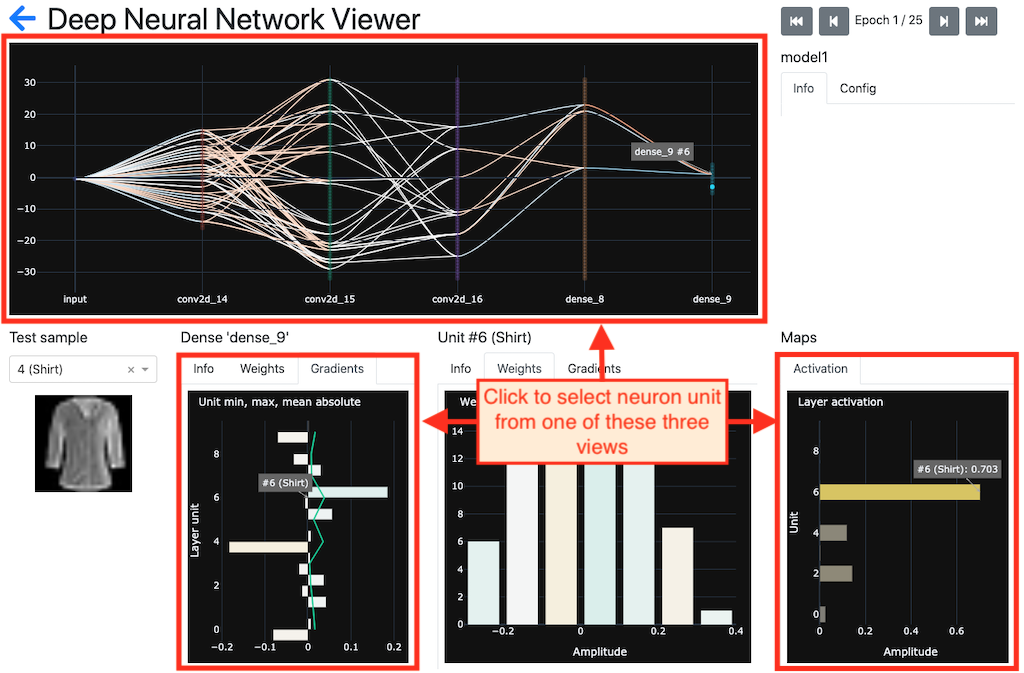
\includegraphics[scale=0.4]{images/dnn-viewer/dnnviewer-selection.png}
    \caption{DNN viewer three panels, from the top panel is selected the training epoch}
    \label{fig:dnn-viewer-top}
\end{figure}

The link between these views is the currently selected layer unit. Selection is made either on the central network view or on the layer weights or gradients figure, or on the layer activation figure (in case of a Dense layer). The selection on the central view will set the layer and unit, whereas the selection on the other views will only update the currently selected unit within the layer. 


\subsubsection{Loading a model}

Model selection is performed through the user interface on the initial page shown on Figure \ref{fig:dnn-viewer-model-selection}.

\begin{figure}[H]
    \centering
    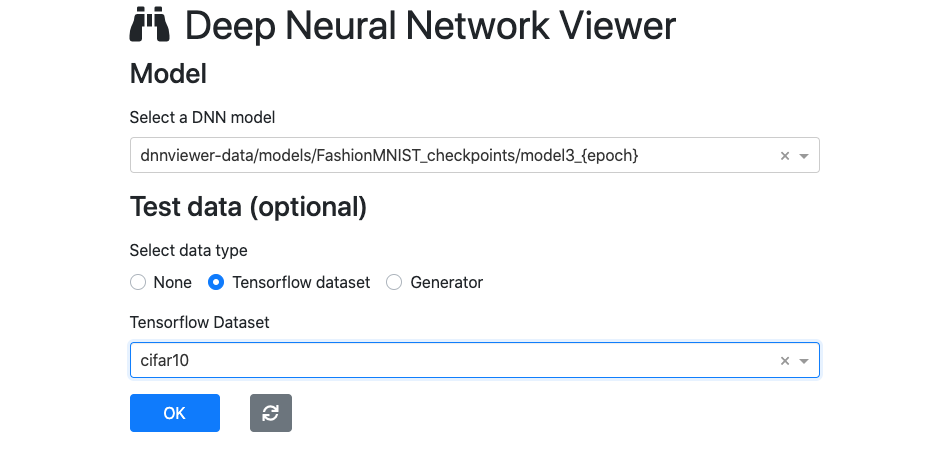
\includegraphics[scale=0.3]{images/dnn-viewer/ModelSelection.png}
    \caption{Model selection in the DNN Viewer GUI}
    \label{fig:dnn-viewer-model-selection}
\end{figure}

The supported model file formats are  HDF5 and Tensorflow checkpoint. Checkpoints can be used as sequences over training epochs if a naming pattern is detected (default pattern is \verb|{model_name}_{epoch}| as illustrated on Figure \ref{fig:dnn-viewer-model-selection} in which the sequence for "model2" is selected).

\subsubsection{Central network view}

This central view is providing at the same time the network architecture and the connections between layers. For each of these two aspects the complexity is raising very quickly with the number of layers, that is why a simplified view is built based on the following choices:
\begin{itemize}
    \item Only the main layers with weights are displayed : fully connected, convolutional layers. The activation, dropout, pooling, batch normalization, upsampling, reshape layers are appended as attributes to previous or following layers. The goal is to decrease the total number of plotted layers and avoid clutter.
    \item Layer connections are showing the main multiplicative weights, starting from the selected layer unit. This algorithm is detailed in \ref{sec-dnnviewer-implementation-topn-connections}
\end{itemize}

This Visualization is very important it must provide the user with some intuitions on what is happening in this dense and complex graph.

\subsubsection{Detailed views}

The bottom panel contains 4 quadrants with detailed views: test data input, layer, unit and maps.

For each of these, there may be alternative views selected through tabs. For example, the layer and unit quadrants have descriptive information in the "Info" tab, and current training parameters in the "Weights" and "Gradients" tab. 

The layer figures are showing three quantities for each of the unit in the layer: minimum, maximum and mean absolute of the values (weights or gradients).

\begin{figure}[H]
    \centering
    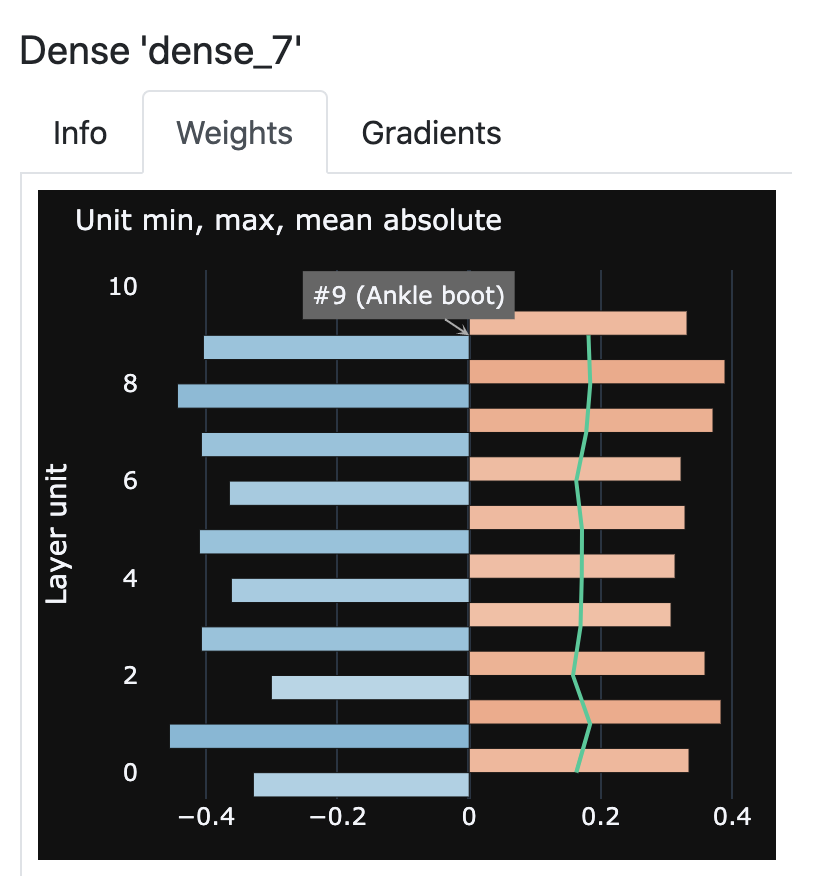
\includegraphics[scale=0.3]{images/dnn-viewer/LayerMinimax.png}
    \caption{Layer view showing min (blue bars), max (red bars) and mean absolute (green multiline) for each of the layer units}
    \label{fig:dnn-viewer-layer-minimax}
\end{figure}


The layer unit figures are different for Dense and convolutional layers: for Dense they are histograms, for convolutional the first filters of the unit are shown.

\begin{figure}[H]
    \centering
    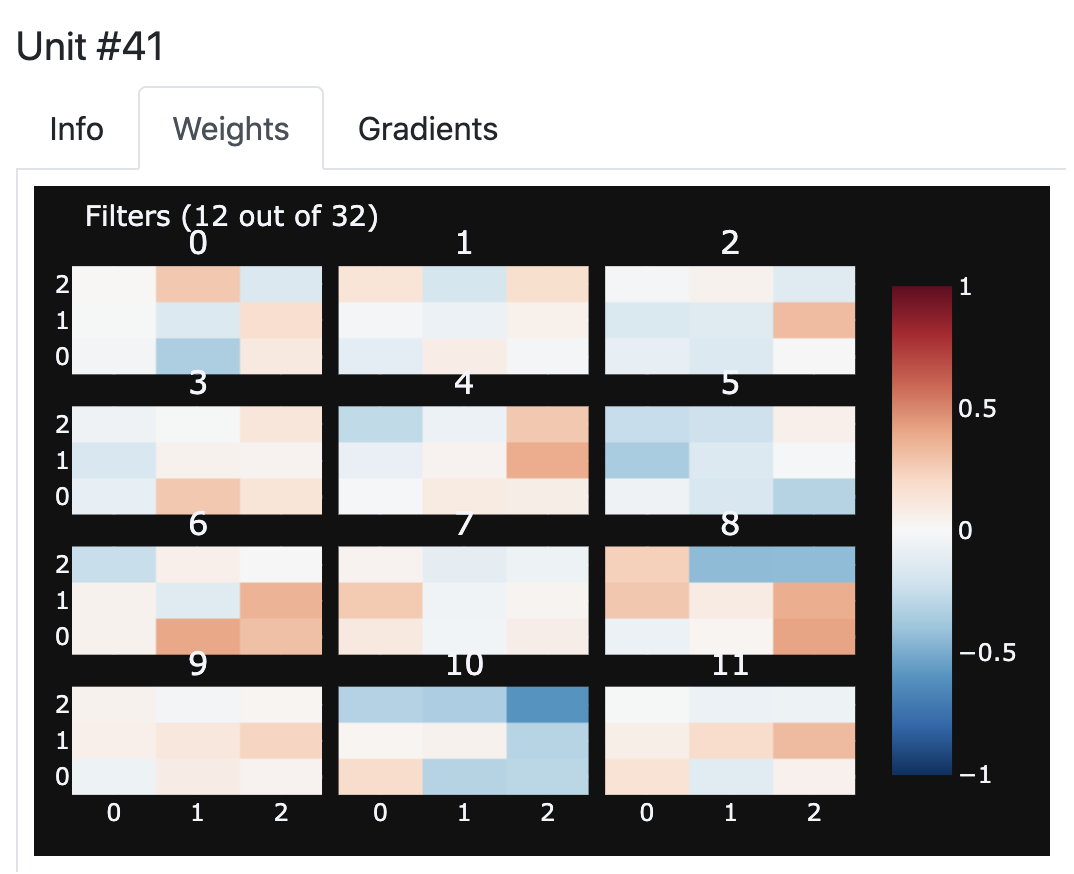
\includegraphics[scale=0.3]{images/dnn-viewer/ConvoFiltersWeights.png}
    \caption{convolutional unit filter view}
    \label{fig:dnn-viewer-unit-convo-filters}
\end{figure}

For the time being, maps are restricted to activation maps, but the saliency maps are in the road-map. 



\subsection{Implementation}
\label{sec-dnnviewer-implementation}


\subsubsection{Software stack (system architecture)}

Starting from a simple visualization on a Jupyter notebook, the DNN Viewer evolved to a client-server web application that reflects its origins and its audience, Data Scientists. The language is Python, the server framework is Plotly Dash, the main dependency is Tensorflow for reading models and evaluating gradients and activations. Dash is generating the client code that relies on Plotly.js and React.js. On the server side, Dash relies on the light web HTTP server Flask. The software stack is depicted on Figure \ref{fig:dnn-viewer-archi1}. The programming paradigm of Dash is tightly linked to the one of React.js: callbacks are fired in reaction to events on the user interface.

Currently, the application code is not state less (as in RESTful paradigm): the model is loaded once, linked to its graphical representation and stays on the server. Moreover, there is no management of user sessions, meaning that only a single user is handled, one model may get loaded at a time. 


\begin{figure}[H]
    \centering
    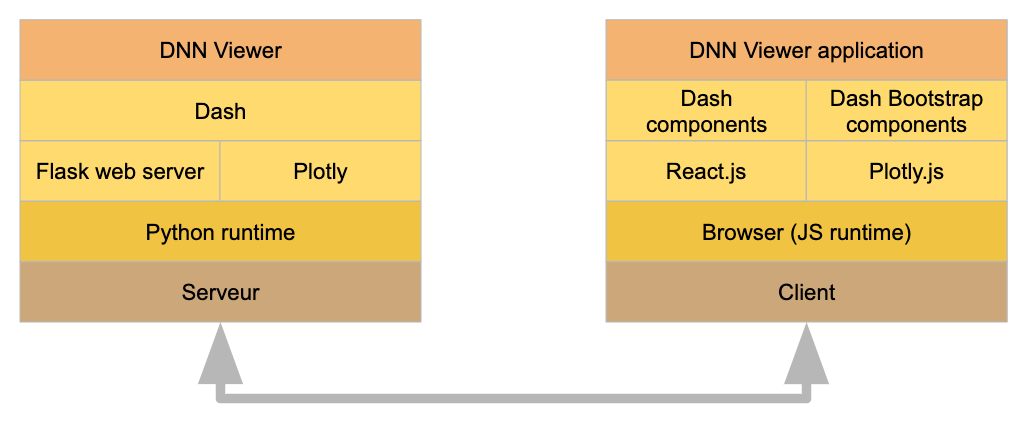
\includegraphics[scale=0.3]{images/dnn-viewer/Architecture.png}
    \caption{DNN viewer software stack}
    \label{fig:dnn-viewer-archi1}
\end{figure}

Main advantages of this environment are a single language (Python) to perform at the same time server processing and client side interaction (necessary Javascript is generated by Dash), and the integration with Plotly, a powerful evolution of Matplotlib. Finally, the install is easy through package management by Pip3.

Drawbacks are a lack of control over the client side events, some limits to Dash when the application has multiple pages (Dash requires all callbacks and bindings to be declared at initialization), and a large dependency on Dash as an open source project that is not so widespread.


\subsubsection{Software architecture}

As many Web applications, the DNN Viewer application is a set of pages that are routed based on events. In Dash, all pages are instantiated at startup in order to create the callbacks. This is done from the main script of DNN Viewer.

The pages are relying on three other components displayed on \ref{fig:dnn-viewer-archi2}:
\begin{itemize}
    \item The Dash application
    \item The \textit{Grapher} which is responsible for the graphical representation of the network and holds a collection of layers
    \item The model sequence which is performing all tasks related to the original model (managing a single or sequence of models, loading the models and creating the layer in the \textit{Grapher}, gradient and saliency computation)
\end{itemize}

\begin{figure}[H]
    \centering
    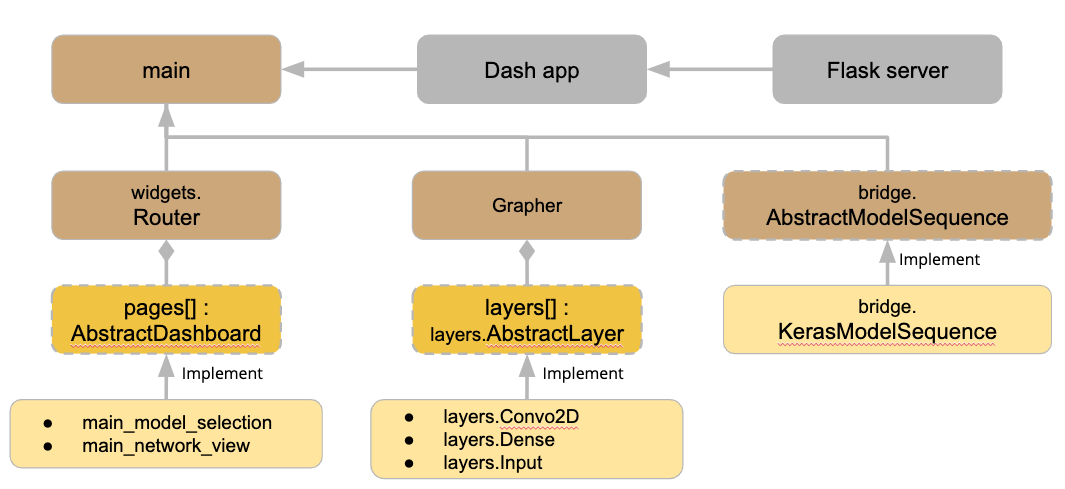
\includegraphics[scale=0.3]{images/dnn-viewer/Architecture2.png}
    \caption{DNN viewer software architecture}
    \label{fig:dnn-viewer-archi2}
\end{figure}


DNN Viewer could be extended to support Pytorch models creating a class specialization of \\
bridge.AbstractModelSequence similar to bridge.KerasModelSequence.


\subsubsection{Visualization of the main connections between layers}
\label{sec-dnnviewer-implementation-topn-connections}

As explained in the overview, the connections between layers are shown as a selection of the weights that link units. There are two main constraints on this visualization, -1- it shall not become over complex, i.e. look as spaghetti, and -2- it shall not take too much computation time since it will be computed at each user selection refresh.

The chosen implementation is taking the currently selected layer neuron unit as focal point. When the application is started, the unit corresponding to the target true class of the first data sample image is automatically selected.

From this focal point, the N weights with the highest absolute value are selected, with N between 1 and 4. This is applied on both sides of the unit: downstream and upstream and propagated to layers through backward and forward propagation. This propagation is taking as focal points the units connected from previous layer. Since N connections are shown at each selected unit, the N units connected are then part of the selection for next layer to layer connection plot, the number of connections grows as a \(N^l\) with \(l\) as the number of layers between the initial layer and the current layer. This number grows very quickly and will simultaneously saturate the visualization and slow down the plot. In order to limit the number of shown connections between two layers, the number of selected (active) units at each layer is arbitrarily capped at 32.

\begin{figure}[H]
    \centering
    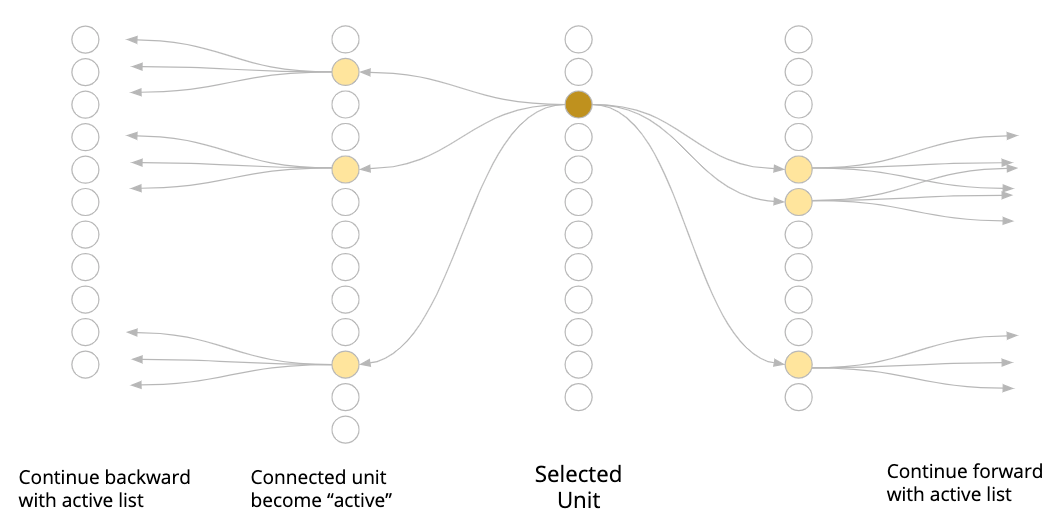
\includegraphics[scale=0.4]{images/dnn-viewer/TopNConnections.png}
    \caption{DNN viewer algorithm to select connections to plot}
    \label{fig:dnn-viewer-topn-connections}
\end{figure}

Each unit to unit connection is plotted as a cubic Bezier curve. The weight strength is plotted as the color of the spline using a divergent color map.

Last but not least complication, when a convolutional layer is connected to a fully connected, there is often an intermediate pseudo layer to "flatten" the tensor at the output of the convolutional layer. It means that the is no one to one connection between the convolutional layer dimension and what is seen as an input dimension on the fully connected layer. This is handled by wrapping the connection number when computing the layer to layer connection plot backward. In the forward pass, there is no such issue. This problem is similar to the one of \ref{embeddings-convolutional}.

\textbf{Discussion on the weight selection:}
\begin{itemize}
    \item For each unit, the selected weights to be plotted are the top N in absolute value. We could argue that given the most used activation function today is ReLU and is asymmetric (truncating negative values), the negative contributions are most-likely discarded. However, there is no direct link between negative contributions and negative weights, it depends on the full forward chain of the network, starting from the image stimuli. For these reasons, the activations are totally ignored in this visualization.
    \item Each layer to layer is evaluated independently starting from the "active list", we could think of a cumulative evaluation that might lead to some weight to vanish as the origin layer is far away. This is area for improvement and might help in keeping low the number of plotted connections, replacing the cap to 32 units in the active list above.
\end{itemize}

\subsubsection{Gradient computation with Keras}

Gradients are not available within the saved model files (HDF5 or Tensorflow checkpoint). They are recomputed from the test data performing a forward prediction with a mini-batch of size 128. The result list of gradient tensor is then affected to each of the layers added to the Grapher.


\subsection{Applied interpretability and findings}

From our experience, there are three main ways to use the DNN Viewer (we expect our users to create and ask for others):
\begin{itemize}
    \item Forward to see the evolution of the feature and manifolds learnt by deeper and deeper layers
    \item Backward, starting from the target true class, inspect the main weights backward and cross inspect with the activation maps
    \item Through time across the training epochs to see the evolution of the strong and weak weights and gradients
\end{itemize}

Each of these is exemplified here below

\subsubsection{Forward inspection}

From [\cite{Erhan2009}] and other studies, it is known that first DNN layers tend to select edges similarly to the Sobel filters, second layer is activated on some specific corners of the input shape or manifold, and deeper layers have more and more abstract and trackable activations. This is also amplified by the lower and lower resolution of the activation images following the chain of pooling layers.

\begin{figure}[H]
    \centering
    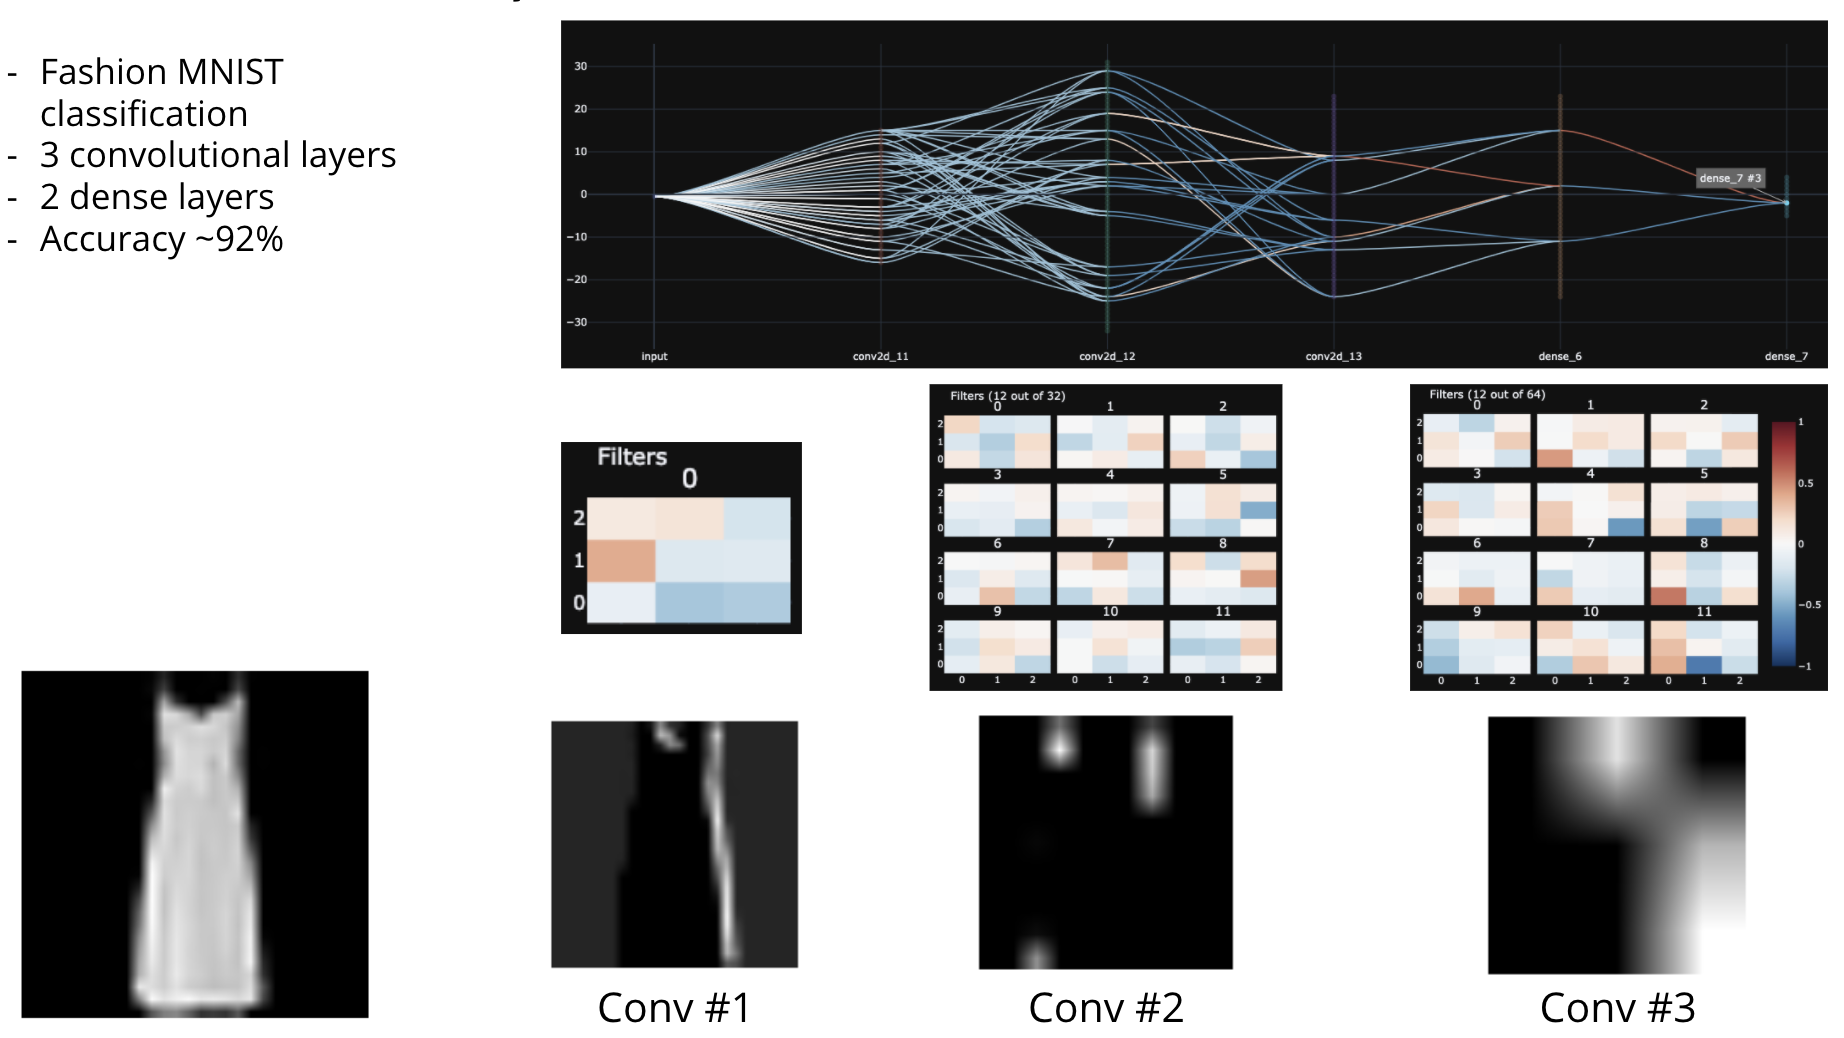
\includegraphics[scale=0.4]{images/dnn-viewer/ForwardDress.png}
    \caption{Forward exploration with a Fashion MNIST dress test image and a simple 5 layer network}
    \label{fig:dnn-viewer-forward-dress}
\end{figure}

Two examples were drawn from a simple DNN to classify Fashion MNIST dataset Figure \ref{fig:dnn-viewer-forward-dress}) and a deeper network handling CIFAR-10 classification (Figure \ref{fig:dnn-viewer-forward-truck}).

The simpler example is showing the progression from edge detection to single region highlights. The larger network is showing a smoother transformation of the input image. The first layer is more like contrast adjustment. The second layer performs the edge detection. On the third and fourth, the truck structure still remains visible but the pooling layer has reinforced the contrast between the image regions of interest and others. On the fifth and sixth, the truck structure is no longer visible and we see some highlighted regions.

\begin{figure}[H]
    \centering
    \includegraphics[scale=0.4]{images/dnn-viewer/TruckForward-Large.png}
    \caption{Forward exploration with a CIFAR-10 test image and a large 9 layer network}
    \label{fig:dnn-viewer-forward-truck}
\end{figure}

Something that is visible in the GUI but not on the extracted pictures is the fact that the simpler DNN has low activations and sharp contracts from the first layer, and the selected connections shown are very often negative whereas the larger model has lower contrast and selected connections are often positive.

We conclude from this inspection that the large model could be optimized to reduce its size in both number of layers and number of units per layer.

\subsubsection{Backward inspection}

For this inspection, the test-case is a LeNet5 network optimized in performance and size using ReLU activations, Dropout regularization, see [\cite{lenet5-optimized}]. There are three convolutional and 2 dense layers. 

From the MNIST Digits dataset, a sample three digit has been selected given the output soft-max probability is only 60\%. The probability for the digit five is close to 40\%. This is shown on Figure \ref{fig:dnn-viewer-backward-1}

\begin{figure}[H]
    \centering
    \includegraphics[scale=0.3]{images/dnn-viewer/BackwardThree_1.png}
    \caption{Backward exploration with a LeNet5, output probabilities for a 3}
    \label{fig:dnn-viewer-backward-1}
\end{figure}

On Figure \ref{fig:dnn-viewer-backward-2}, looking at previous layer on the highlighted main negative contribution (unit \#32), it is observed that this unit contributes positively to the softmax probability for the digit 1. Also, there is no activation on this unit for the digit three at the input.

\begin{figure}[H]
    \centering
    \includegraphics[scale=0.3]{images/dnn-viewer/BackwardThree_2.png}
    \caption{Backward exploration with a LeNet5, layer before the softmax with digit three input}
    \label{fig:dnn-viewer-backward-2}
\end{figure}

The positive contribution to digit 1 of unit \#32 the pre-softmax layer is confirmed on Figure \ref{fig:dnn-viewer-backward-3}

\begin{figure}[H]
    \centering
    \includegraphics[scale=0.3]{images/dnn-viewer/BackwardThree_3.png}
    \caption{Backward exploration with a LeNet5, layer before the softmax with digit one input}
    \label{fig:dnn-viewer-backward-3}
\end{figure}

Selecting again the digit 3 sample, the main contribution to the digit 5 softmax probability is inspected: unit 39 of the pre-softmax layer, Figure \ref{fig:dnn-viewer-backward-4}. The activation of the input digit three is measured to be quite high for on this unit.

\begin{figure}[H]
    \centering
    \includegraphics[scale=0.3]{images/dnn-viewer/BackwardThree_4.png}
    \caption{Backward exploration with a LeNet5, layer before the softmax, main positive contribution to digit five}
    \label{fig:dnn-viewer-backward-4}
\end{figure}

Jumping to the last convolutional layer, unit \#0 is selected. It shows a activation on two horizontal bars of the input three, Figure {fig:dnn-viewer-backward-5}. There seems to be a positive contribution to the softmax for digit three through unit \#31 of pre-softmax layer and a negative contribution through unit \#4 of the same layer.

\begin{figure}[H]
    \centering
    \includegraphics[scale=0.3]{images/dnn-viewer/BackwardThree_5.png}
    \caption{Backward exploration with a LeNet5, last convolutional layer, unit \#0}
    \label{fig:dnn-viewer-backward-5}
\end{figure}

The positive contribution is confirmed on Figure \ref{fig:dnn-viewer-backward-6}. The negative contribution is not activating on the input digit three, that's probably the action of the ReLU activation function, Figure \ref{fig:dnn-viewer-backward-7}.

\begin{figure}[H]
    \centering
    \includegraphics[scale=0.3]{images/dnn-viewer/BackwardThree_6.png}
    \caption{Backward exploration with a LeNet5, pre-softmax layer, unit \#31}
    \label{fig:dnn-viewer-backward-6}
\end{figure}

\begin{figure}[H]
    \centering
    \includegraphics[scale=0.3]{images/dnn-viewer/BackwardThree_7.png}
    \caption{Backward exploration with a LeNet5, pre-softmax layer, unit \#4}
    \label{fig:dnn-viewer-backward-7}
\end{figure}

With this inspection, we have shown the potential of the DNN Viewer to quickly check and track the output of the network in order to understand some failures or fragile results. However, it has been quite difficult to find positive contributions to the softmax property being probed. In fact, the main view is showing only the top 3 main weights in absolute value, in this case all negative, and the layer weights are presented in the bottom panel as an histogram. This is room for improvement, one idea would be to add another view in this quadrant that mixes weights and activations to provide weighted contributions.

\subsubsection{Inspection over epochs}

For this inspection, used DNN is a classifier for the MNIST Fashion based on the Keras tutorial on CNN [\cite{keras-tutorial-cnn}]. This model was trained over 25 epochs as it is missing regularization, it is over-fitting as shown on Figure \ref{fig:dnn-viewer-time-training}.

\begin{figure}[H]
    \centering
    \includegraphics[scale=0.3]{images/dnn-viewer/Fashion-MNIST_Training.png}
    \caption{Training of the simple Fashion MNIST model}
    \label{fig:dnn-viewer-time-training}
\end{figure}

Using DNN Viewer, the activation of a test Shirt image is observed. Initially, softmax probability for the test sample is 70\% on the Shirt class. The gradient for the corresponding unit is relatively positive compared to other units of this layer.

\begin{figure}[H]
    \centering
    \includegraphics[scale=0.3]{images/dnn-viewer/TimeShirt_epoch1.png}
    \caption{Activation and weights for a Shirt test sample at epoch 1}
    \label{fig:dnn-viewer-time-shirt-epoch1}
\end{figure}

At the end of the epoch 2, the softmax probability has increased, gradient is still high.

\begin{figure}[H]
    \centering
    \includegraphics[scale=0.3]{images/dnn-viewer/TimeShirt_epoch3.png}
    \caption{Activation and weights for a Shirt test sample at epoch 2}
    \label{fig:dnn-viewer-time-shirt-epoch2}
\end{figure}

But at epoch 3, the softmax probability has decreased and the gradient is now mostly positive.

\begin{figure}[H]
    \centering
    \includegraphics[scale=0.3]{images/dnn-viewer/TimeShirt_epoch3.png}
    \caption{Activation and weights for a Shirt test sample at epoch 3}
    \label{fig:dnn-viewer-time-shirt-epoch3}
\end{figure}

At epoch 4, the probability is raising again, gradients are more balanced.

\begin{figure}[H]
    \centering
    \includegraphics[scale=0.3]{images/dnn-viewer/TimeShirt_epoch4.png}
    \caption{Activation and weights for a Shirt test sample at epoch 4}
    \label{fig:dnn-viewer-time-shirt-epoch4}
\end{figure}

At epoch 5, the gradients are mostly positive and the probability is raising close to 90\%.

\begin{figure}[H]
    \centering
    \includegraphics[scale=0.3]{images/dnn-viewer/TimeShirt_epoch5.png}
    \caption{Activation and weights for a Shirt test sample at epoch 5}
    \label{fig:dnn-viewer-time-shirt-epoch5}
\end{figure}

Jumping at epoch 8, the probability is a little lower, gradient are in majority at 0.

\begin{figure}[H]
    \centering
    \includegraphics[scale=0.3]{images/dnn-viewer/TimeShirt_epoch8.png}
    \caption{Activation and weights for a Shirt test sample at epoch 8}
    \label{fig:dnn-viewer-time-shirt-epoch8}
\end{figure}

Jumping at epoch 15, the probability is very high at 96\%, gradient are in majority at 0, extrema are at +- 0.05.

\begin{figure}[H]
    \centering
    \includegraphics[scale=0.3]{images/dnn-viewer/TimeShirt_epoch15.png}
    \caption{Activation and weights for a Shirt test sample at epoch 15}
    \label{fig:dnn-viewer-time-shirt-epoch15}
\end{figure}

Eventually, at epoch 25, the performance is very good with a 99\% probability but the gradients extrema are still in the range of +- 0.1. We may think that the convergence is not completed, this is a consequence of the over-fitting.

\begin{figure}[H]
    \centering
    \includegraphics[scale=0.3]{images/dnn-viewer/TimeShirt_epoch25.png}
    \caption{Activation and weights for a Shirt test sample at epoch 25}
    \label{fig:dnn-viewer-time-shirt-epoch25}
\end{figure}



\subsection{DNN Viewer improvements and new features in P4}

During the last period, the DNN Viewer has been refined with many bug fixes and with improvements to support more models. Opening DNN Viewer as a generic tool to view saved models is quite a challenge given the huge amount of options on layers (strides, regularizations), the many types of layers (dense, convolutional 1D/2D/3D, pooling max/average 1D/2D/3D, activations, batch normalization...), the versions of Tensorflow (2.0, 2.1, 2.2) and format types (HDF5, checkpoints). The coming version of DNN Viewer is much stronger and versatile even if still not supporting all layer types.

During the period, the scope of the DNN Viewer has been enlarged with the following features and tests:
\begin{itemize}
    \item More descriptive properties to the network and to the layers
    \item Support for Tensorflow Data-sets
    \item Support for more layers, enabling GAN networks (including the Sequential within Sequential topology)
\end{itemize}


\begin{figure}[H]
    \centering
    \includegraphics[scale=0.3]{images/dnn-viewer/CIFAR10+Random.png}
    \caption{Using the random generator as input on a CIFAR10 classifier is showing that class 1 (car) has probability 1, this result is reproducible. Does it mean that random noise is a car?}
    \label{fig:dnn-viewer-random-generator-cifar10}
\end{figure}

We have also been looking for feedback from users. A survey has been submitted to the students of the MS BigData, and to the machine learning teachers. Two students and two teachers have answered to the survey, among which two have succesfully tested the software, and with high interest. The main shared feedback is to provide more datasets, or capabilities to load personal datasets. Looking at the online feedback, even if Pipy is reporting more than 1000 downloads per mont since April, DNN Viewer is still looking for its public and more communication is required to advertise it.



\subsection{DNN Viewer next steps}

The DNN viewer is now an open source project on Github [\cite{dnnviewer2020}] and the package is distributed through Pip.org [\cite{dnnviewer-pypi2020}]. You may already install it and try it with your own "baby models".

As said in previous section, DNN Viewer needs to find a public of users, and ultimatly a community. Along with the improvements listed below, we will actively promote it on the Internet. The first step being a publication on Medium to present the software, its capabilities.

Incremental improvements:
\begin{itemize}
    \item Saliency as an alternative to activation maps
    \item More configuration to the views and better view when the view is complex (e.g. convolutional unit filter number may be large)
    \item Training loss and metrics Graphs
    \item Support for personal data-sets
    \item Improve on the visualization of the contributions as suggested above
\end{itemize}

Extensions to the tool:
\begin{itemize}
    \item Support for more complex architectures like residual networks
    \item Support for other tasks: NLP, time series, recurrent networks...
    \item More complex views and statistics that would require asynchronous server processing: UMAP (see \ref{sec5}), Intersection over Union [\cite{Zhou2017}]
\end{itemize}

Last but probably not least, at this point in the software development of DNN Viewer, we think that Dash is probably not the best tool to design a complete single page application, we are thinking of rebuilding it in a two tier architecture with Flask on the server, and a client side (browser) app built directly on React.js and Plotly.js. % DNN Viewer
\newpage

\section{Conclusion}
\label{conclusion}

This project gave us a unique opportunity to explore in-depth convolutional neural networks. We started with a thorough study of CNN, their applications, and also their limitations and weaknesses. This led us to consider the recent scientific litterature on diverse subjects such as saliency maps, dimension reduction, adversarial neural networks, and visualization atlasses.

Based on the requests of our partner, we then decided to focus the project more specifically on visualization.  Because this concept is fairly large in scope, and because there exist different ways to tackle the visualization of a neural network, we thought the best decision was to develop several applications, each centered on one specific approach.

The first application is the DNN-Monitor. Its principal objective consists in monitoring a CNN in the course of the training. It provides visualizations for essential metrics determining the quality of a training: loss and accuracy functions, weights and gradients, and activations along with their correlations.

The second application is the Deep Embedding Viewer. It starts from the principle that it is difficult to visualize a network at the scale of individual elements as soon as the network becomes even moderately large. For this reason, it adopts a dimension reduction approach, relying on modern techniques such as t-SNE or UMAP. It then proposes 2d visualizations that provide a view on class separation and the spatial location of individua images.

The final tool proposed for the project is the DNN-Viewer. It proposes to abstract from a specific layer of the model to adopt a more global approach that provides a full overview of the CNN as a combination of interrelated layers. It places the emphasis on the activations across layers, providing for instance custom visualizations on the most important transmission chanels within the network.

Visualizing and interpreting neural networks currently represents a major axis of scientific research. There is thus much potential for further research and developments. This might prove challenging however since our industrial partner, the Ministry of Defense, has not provided us with feedback so far. Still, we may propose the following tracks to pursue the project:

 \begin{itemize}
	\item gather all the applications developed within a single unified software. The material constraints and the exceptional nature of this year's situation has rendered difficult the parallel creations of multiple applications and their integration in a single framework. Ideally however, it would prove more user-friendly to operate all the functionalities from a single programme.
	\item integrate the research subjects that were studied during the first step of the project in our tools. That might for instance include saliency maps and adversarial attacks.
	\item develop further metrics to assess with a maximum of efficiency whether a training is satisfactory, or wether a visualization provides useful hints about the network, its structure and its decisions.
	\item explore and generalize the tools developed to other architectures and datasets. So far the project has focused on relatively standard architectures and datasets. Yet a natural step would imply the extension of our tools to a wider range of models. This might create new challenges, as alternative architectures may also imply the conception of new representations.
	\item consider how to make sure that the visualizations are scale-robust. Screen space remains limited, even though CNN tend to get larger and larger. This question may become predominant to adequaltely visualize architectures that now include dozens of millions of parameters.
\end{itemize}



 % DNN Viewer
\pagebreak


%--------------------
%    bibliography   -
%--------------------


\bibliography{sections/bibliography}

\end{document}